\documentclass[DM,lsstdraft,STR,toc]{lsstdoc}
\usepackage{geometry}
\usepackage{longtable,booktabs}
\usepackage{enumitem}
\usepackage{arydshln}

\input meta.tex

\providecommand{\tightlist}{
  \setlength{\itemsep}{0pt}\setlength{\parskip}{0pt}}

\setcounter{tocdepth}{4}

\begin{document}

\def\milestoneName{Fall 2019 Pipelines Release Acceptance Test Campaign}
\def\milestoneId{LVV-P65}
\def\product{Acceptance}

\setDocCompact{true}

\title{ LVV-P65 Fall 2019 Pipelines Release Acceptance Test Campaign Test Plan and Report}
\setDocRef{\lsstDocType-\lsstDocNum}
\date{\vcsdate}
\setDocUpstreamLocation{\url{https://github.com/lsst/lsst-texmf/examples}}
\author{ Jeffrey Carlin }

\input history_and_info.tex


\setDocAbstract{
This is the test plan and report for LVV-P65 (Fall 2019 Pipelines Release Acceptance Test Campaign),
an LSST level 2 milestone pertaining to the Data Management Subsystem.
}


\maketitle

\section{Introduction}
\label{sect:intro}


\subsection{Objectives}
\label{sect:objectives}

 This Acceptance Test campaign aims to verify a small number of
\href{https://lse-61.lsst.io/}{DMSR} (\citeds{LSE-61}) requirements related to
the LSST Science Pipelines. It will be executed in conjunction with the
release of Science Pipelines Version 19.0.0, but the pipeline release is
not contingent upon this test campaign. This Test Plan aims to
demonstrate that the included requirements have been met by Version
19.0.0 of the Pipelines, and to thus fully verify their completion and
readiness for LSST Operations.



\subsection{System Overview}
\label{sect:systemoverview}

 The tests to be executed are intended to verify that the DM system
satisfies a subset of the requirements outlined in the Data Management
System Requirements (DMSR; \href{https://lse-61.lsst.io/}{LSE-61} ).
This subset of requirements is related to pipeline algorithms, and was
selected for this campaign to coincide with the release of a new version
of the LSST Science Pipelines. Additional DMSR requirements will be
verified in later Acceptance Test
Campaigns.\\[2\baselineskip]\textbf{Applicable
Documents:}\\[2\baselineskip]\citeds{LSE-61} Data Management System
Requirements\\
\citeds{LDM-503} Data Management Test Plan\\[2\baselineskip]The tests will be
performed using the HSC-RC2 dataset (as defined in
\href{https://jira.lsstcorp.org/browse/DM-11345}{DM-11345} ). When
possible, we will start our tests with the data products resulting from
processing HSC-RC2 with the w\_2019\_46 weekly pipelines release (
\href{https://jira.lsstcorp.org/browse/DM-22223}{DM-22223} ) that was
used to create v19 of the Science Pipelines.~


\subsection{Document Overview}
\label{sect:docoverview}

This document was generated from Jira, obtaining the relevant information from the 
\href{https://jira.lsstcorp.org/secure/Tests.jspa#/testPlan/LVV-P65}{LVV-P65}
~Jira Test Plan and related Test Cycles (
  \href{https://jira.lsstcorp.org/secure/Tests.jspa#/testCycle/LVV-C115}{LVV-C115}
).

Section \ref{sect:intro} provides an overview of the test campaign, the system under test (\product{}),
the applicable documentation, and explains how this document is organized.
Section \ref{sect:configuration}  describes the configuration used for this test.
Section \ref{sect:personnel} describes the necessary roles and lists the individuals assigned to them.
%Section \ref{sect:plannedtestactivities} provides the list of planned test cycles and test cases,
including all relevant information that fully describes the test campaign.

Section \ref{sect:overview} provides a summary of the test results, including an overview in Table \ref{table:summary},
an overall assessment statement and suggestions for possible improvements.
Section \ref{sect:detailedtestresults} provides detailed results for each step in each test case.

The current status of test plan LVV-P65 in Jira is \textbf{ Approved }.

\subsection{References}
\label{sect:references}
\renewcommand{\refname}{}
\bibliography{lsst,refs,books,refs_ads}
\section{Test Configuration}
\label{sect:configuration}

\subsection{Data Collection}

  Observing is not required for this test campaign.

\subsection{Verification Environment}
\label{sect:hwconf}
   The ``lsst-lsp-stable'' instance of the LSST Science Platform (LSP),
hosted at the LDF, and the ``lsst-dev'' development cluster at NCSA.~In
particular, we will use Release 19.0.0 of the Pipelines, whose release
is DM Milestone LDM-503-11b (Test Plan located
\href{https://jira.lsstcorp.org/secure/Tests.jspa\#/testPlan/LVV-P62}{here)}.


  \subsection{Entry Criteria}
   Release and availability of Science Pipelines version 19.




\newpage
\section{Personnel}
\label{sect:personnel}

The personnel involved in the test campaign are shown in the following table.

\begin{longtable}{p{3cm}p{3cm}p{3cm}p{6cm}}
\hline
\multicolumn{2}{r}{Test Plan (LVV-P65) owner:} &
\multicolumn{2}{l}{\textbf{ Jeffrey Carlin } }\\\hline
\multicolumn{2}{r}{ LVV-C115 owner:} &
\multicolumn{2}{l}{\textbf{
    Jeffrey Carlin
}
} \\\hline
\textbf{Test Case} & \textbf{Assigned to} & \textbf{Executed by} & \textbf{Additional Test Personnel} \\ \hline
\href{https://jira.lsstcorp.org/secure/Tests.jspa#/testCase/LVV-T41}{LVV-T41}
& {\small Jim Bosch } & {\small Jeffrey Carlin } &
\begin{minipage}[]{6cm}
\smallskip
{\small  }
\medskip
\end{minipage}
\\ \hline
\href{https://jira.lsstcorp.org/secure/Tests.jspa#/testCase/LVV-T62}{LVV-T62}
& {\small Jim Bosch } & {\small Jeffrey Carlin } &
\begin{minipage}[]{6cm}
\smallskip
{\small  }
\medskip
\end{minipage}
\\ \hline
\href{https://jira.lsstcorp.org/secure/Tests.jspa#/testCase/LVV-T40}{LVV-T40}
& {\small Jim Bosch } & {\small Jeffrey Carlin } &
\begin{minipage}[]{6cm}
\smallskip
{\small  }
\medskip
\end{minipage}
\\ \hline
\href{https://jira.lsstcorp.org/secure/Tests.jspa#/testCase/LVV-T1240}{LVV-T1240}
& {\small Jim Bosch } & {\small Jeffrey Carlin } &
\begin{minipage}[]{6cm}
\smallskip
{\small  }
\medskip
\end{minipage}
\\ \hline
\href{https://jira.lsstcorp.org/secure/Tests.jspa#/testCase/LVV-T28}{LVV-T28}
& {\small Colin Slater } & {\small Jeffrey Carlin } &
\begin{minipage}[]{6cm}
\smallskip
{\small  }
\medskip
\end{minipage}
\\ \hline
\href{https://jira.lsstcorp.org/secure/Tests.jspa#/testCase/LVV-T43}{LVV-T43}
& {\small Jim Bosch } & {\small Jeffrey Carlin } &
\begin{minipage}[]{6cm}
\smallskip
{\small  }
\medskip
\end{minipage}
\\ \hline
\href{https://jira.lsstcorp.org/secure/Tests.jspa#/testCase/LVV-T132}{LVV-T132}
& {\small Robert Gruendl } & {\small Jeffrey Carlin } &
\begin{minipage}[]{6cm}
\smallskip
{\small  }
\medskip
\end{minipage}
\\ \hline
\href{https://jira.lsstcorp.org/secure/Tests.jspa#/testCase/LVV-T1745}{LVV-T1745}
& {\small Jeffrey Carlin } & {\small Jeffrey Carlin } &
\begin{minipage}[]{6cm}
\smallskip
{\small  }
\medskip
\end{minipage}
\\ \hline
\href{https://jira.lsstcorp.org/secure/Tests.jspa#/testCase/LVV-T1746}{LVV-T1746}
& {\small Jeffrey Carlin } & {\small Jeffrey Carlin } &
\begin{minipage}[]{6cm}
\smallskip
{\small  }
\medskip
\end{minipage}
\\ \hline
\href{https://jira.lsstcorp.org/secure/Tests.jspa#/testCase/LVV-T1747}{LVV-T1747}
& {\small Jeffrey Carlin } & {\small Jeffrey Carlin } &
\begin{minipage}[]{6cm}
\smallskip
{\small  }
\medskip
\end{minipage}
\\ \hline
\href{https://jira.lsstcorp.org/secure/Tests.jspa#/testCase/LVV-T1748}{LVV-T1748}
& {\small Jeffrey Carlin } & {\small Jeffrey Carlin } &
\begin{minipage}[]{6cm}
\smallskip
{\small  }
\medskip
\end{minipage}
\\ \hline
\href{https://jira.lsstcorp.org/secure/Tests.jspa#/testCase/LVV-T1749}{LVV-T1749}
& {\small Jeffrey Carlin } & {\small Jeffrey Carlin } &
\begin{minipage}[]{6cm}
\smallskip
{\small  }
\medskip
\end{minipage}
\\ \hline
\href{https://jira.lsstcorp.org/secure/Tests.jspa#/testCase/LVV-T1750}{LVV-T1750}
& {\small Jeffrey Carlin } & {\small Jeffrey Carlin } &
\begin{minipage}[]{6cm}
\smallskip
{\small  }
\medskip
\end{minipage}
\\ \hline
\href{https://jira.lsstcorp.org/secure/Tests.jspa#/testCase/LVV-T1751}{LVV-T1751}
& {\small Jeffrey Carlin } & {\small Jeffrey Carlin } &
\begin{minipage}[]{6cm}
\smallskip
{\small  }
\medskip
\end{minipage}
\\ \hline
\href{https://jira.lsstcorp.org/secure/Tests.jspa#/testCase/LVV-T1752}{LVV-T1752}
& {\small Jeffrey Carlin } & {\small Jeffrey Carlin } &
\begin{minipage}[]{6cm}
\smallskip
{\small  }
\medskip
\end{minipage}
\\ \hline
\href{https://jira.lsstcorp.org/secure/Tests.jspa#/testCase/LVV-T1753}{LVV-T1753}
& {\small Jeffrey Carlin } & {\small Jeffrey Carlin } &
\begin{minipage}[]{6cm}
\smallskip
{\small  }
\medskip
\end{minipage}
\\ \hline
\href{https://jira.lsstcorp.org/secure/Tests.jspa#/testCase/LVV-T1754}{LVV-T1754}
& {\small Jeffrey Carlin } & {\small Jeffrey Carlin } &
\begin{minipage}[]{6cm}
\smallskip
{\small  }
\medskip
\end{minipage}
\\ \hline
\href{https://jira.lsstcorp.org/secure/Tests.jspa#/testCase/LVV-T1755}{LVV-T1755}
& {\small Jeffrey Carlin } & {\small Jeffrey Carlin } &
\begin{minipage}[]{6cm}
\smallskip
{\small  }
\medskip
\end{minipage}
\\ \hline
\href{https://jira.lsstcorp.org/secure/Tests.jspa#/testCase/LVV-T1758}{LVV-T1758}
& {\small Jeffrey Carlin } & {\small Jeffrey Carlin } &
\begin{minipage}[]{6cm}
\smallskip
{\small  }
\medskip
\end{minipage}
\\ \hline
\href{https://jira.lsstcorp.org/secure/Tests.jspa#/testCase/LVV-T1759}{LVV-T1759}
& {\small Jeffrey Carlin } & {\small Jeffrey Carlin } &
\begin{minipage}[]{6cm}
\smallskip
{\small  }
\medskip
\end{minipage}
\\ \hline
\end{longtable}

\newpage

\section{Test Campaign Overview}
\label{sect:overview}

\subsection{Summary}
\label{sect:summarytable}

\begin{longtable}{p{2cm}p{2.5cm}p{9cm}p{2.5cm}}
\toprule
\multicolumn{3}{l}{ Test Plan {\bf LVV-P65:  Fall 2019 Pipelines Release Acceptance Test Campaign
 }} & Approved \\\hline

  \multicolumn{3}{l}{ Test Cycle {\bf LVV-C115:  Fall 2019 Pipelines Release Acceptance Test Campaign
 }} & Done \\\hline

  {\bf \footnotesize test case} & {\bf \footnotesize status} & {\bf \footnotesize comment} & {\bf \footnotesize issues} \\\toprule

\href{https://jira.lsstcorp.org/secure/Tests.jspa#/testCase/LVV-T41}{LVV-T41}
    & Pass &
    \begin{minipage}[]{9cm}
    \smallskip
     Test executed on lsst-lsp-stable, using Release v19.0.0, with a Large
container.

    \medskip
    \end{minipage}
    &
    \\\hline
\href{https://jira.lsstcorp.org/secure/Tests.jspa#/testCase/LVV-T62}{LVV-T62}
    & Pass &
    \begin{minipage}[]{9cm}
    \smallskip
     Test executed on lsst-lsp-stable, using Release v19.0.0, with a Large
container.

    \medskip
    \end{minipage}
    &
    \\\hline
\href{https://jira.lsstcorp.org/secure/Tests.jspa#/testCase/LVV-T40}{LVV-T40}
    & Pass w/ Deviation &
    \begin{minipage}[]{9cm}
    \smallskip
     Test executed on lsst-lsp-stable, using Release v19.0.0, with a Large
container.

    \medskip
    \end{minipage}
    &
    \\\hline
\href{https://jira.lsstcorp.org/secure/Tests.jspa#/testCase/LVV-T1240}{LVV-T1240}
    & Pass &
    \begin{minipage}[]{9cm}
    \smallskip
     Test executed on lsst-lsp-stable, using Release v19.0.0, with a Large
container.

    \medskip
    \end{minipage}
    &
    \\\hline
\href{https://jira.lsstcorp.org/secure/Tests.jspa#/testCase/LVV-T28}{LVV-T28}
    & Pass w/ Deviation &
    \begin{minipage}[]{9cm}
    \smallskip
     Test executed on lsst-lsp-stable, using Release v19.0.0, with a Large
container.

    \medskip
    \end{minipage}
    &
    \\\hline
\href{https://jira.lsstcorp.org/secure/Tests.jspa#/testCase/LVV-T43}{LVV-T43}
    & Pass &
    \begin{minipage}[]{9cm}
    \smallskip
     Test executed on lsst-lsp-stable, using Release v19.0.0, with a Large
container.

    \medskip
    \end{minipage}
    &
    \\\hline
\href{https://jira.lsstcorp.org/secure/Tests.jspa#/testCase/LVV-T132}{LVV-T132}
    & Pass &
    \begin{minipage}[]{9cm}
    \smallskip
    
    \medskip
    \end{minipage}
    &
    \\\hline
\href{https://jira.lsstcorp.org/secure/Tests.jspa#/testCase/LVV-T1745}{LVV-T1745}
    & Pass &
    \begin{minipage}[]{9cm}
    \smallskip
     Tests executed on lsst-dev, using Release v19.0.0.

    \medskip
    \end{minipage}
    &
    \\\hline
\href{https://jira.lsstcorp.org/secure/Tests.jspa#/testCase/LVV-T1746}{LVV-T1746}
    & Pass &
    \begin{minipage}[]{9cm}
    \smallskip
     Tests executed on lsst-dev, using Release v19.0.0.

    \medskip
    \end{minipage}
    &
    \\\hline
\href{https://jira.lsstcorp.org/secure/Tests.jspa#/testCase/LVV-T1747}{LVV-T1747}
    & Pass &
    \begin{minipage}[]{9cm}
    \smallskip
     Tests executed on lsst-dev, using Release v19.0.0.

    \medskip
    \end{minipage}
    &
    \\\hline
\href{https://jira.lsstcorp.org/secure/Tests.jspa#/testCase/LVV-T1748}{LVV-T1748}
    & Pass &
    \begin{minipage}[]{9cm}
    \smallskip
     Tests executed on lsst-dev, using Release v19.0.0.

    \medskip
    \end{minipage}
    &
    \\\hline
\href{https://jira.lsstcorp.org/secure/Tests.jspa#/testCase/LVV-T1749}{LVV-T1749}
    & Pass &
    \begin{minipage}[]{9cm}
    \smallskip
     Tests executed on lsst-dev, using Release v19.0.0.

    \medskip
    \end{minipage}
    &
    \\\hline
\href{https://jira.lsstcorp.org/secure/Tests.jspa#/testCase/LVV-T1750}{LVV-T1750}
    & Pass &
    \begin{minipage}[]{9cm}
    \smallskip
     Tests executed on lsst-dev, using Release v19.0.0.

    \medskip
    \end{minipage}
    &
    \\\hline
\href{https://jira.lsstcorp.org/secure/Tests.jspa#/testCase/LVV-T1751}{LVV-T1751}
    & Pass &
    \begin{minipage}[]{9cm}
    \smallskip
     Tests executed on lsst-dev, using Release v19.0.0.

    \medskip
    \end{minipage}
    &
    \\\hline
\href{https://jira.lsstcorp.org/secure/Tests.jspa#/testCase/LVV-T1752}{LVV-T1752}
    & Pass &
    \begin{minipage}[]{9cm}
    \smallskip
     Tests executed on lsst-dev, using Release v19.0.0.

    \medskip
    \end{minipage}
    &
    \\\hline
\href{https://jira.lsstcorp.org/secure/Tests.jspa#/testCase/LVV-T1753}{LVV-T1753}
    & Pass &
    \begin{minipage}[]{9cm}
    \smallskip
     Tests executed on lsst-dev, using Release v19.0.0.

    \medskip
    \end{minipage}
    &
    \\\hline
\href{https://jira.lsstcorp.org/secure/Tests.jspa#/testCase/LVV-T1754}{LVV-T1754}
    & Pass &
    \begin{minipage}[]{9cm}
    \smallskip
     Tests executed on lsst-dev, using Release v19.0.0.

    \medskip
    \end{minipage}
    &
    \\\hline
\href{https://jira.lsstcorp.org/secure/Tests.jspa#/testCase/LVV-T1755}{LVV-T1755}
    & Pass &
    \begin{minipage}[]{9cm}
    \smallskip
     Tests executed on lsst-dev, using Release v19.0.0.

    \medskip
    \end{minipage}
    &
    \\\hline
\href{https://jira.lsstcorp.org/secure/Tests.jspa#/testCase/LVV-T1758}{LVV-T1758}
    & Fail &
    \begin{minipage}[]{9cm}
    \smallskip
     Tests executed on lsst-dev, using Release v19.0.0.

    \medskip
    \end{minipage}
    &
    \\\hline
\href{https://jira.lsstcorp.org/secure/Tests.jspa#/testCase/LVV-T1759}{LVV-T1759}
    & Pass &
    \begin{minipage}[]{9cm}
    \smallskip
     Tests executed on lsst-dev, using Release v19.0.0.

    \medskip
    \end{minipage}
    &
    \\\hline
\caption{Test Campaign Summary}
\label{table:summary}
\end{longtable}

\subsection{Overall Assessment}
\label{sect:overallassessment}

 This campaign successfully demonstrated that the DM system is meeting
many of its requirements, primarily using the HSC-RC2 dataset. The
requirements that were verified include some related to basic image
processing and data products (e.g., PSF and background modeling,
astrometric solutions and WCS), and a number of tests related to DM
algorithms provided to calculate performance metrics. (Note that the DM
system is not required to verify that the performance metrics are
meeting their required thresholds, but simply that DM must provide the
tools to calculate/evaluate the metrics.) The tests demonstrated that a
subset of these metrics can be measured at present, and that the
framework (namely, `validate\_drp`) exists to enable the addition of
other metrics.\\[2\baselineskip]Some minor issues that arose include:

\begin{itemize}
\tightlist
\item
  `validate\_drp` -- while powerful and essential to this test campaign
  -- can be challenging to work with, and its architecture may make it
  difficult to implement some of the more complicated metrics in the
  future.
\item
  It may be difficult to scale up `validate\_drp` to run on larger
  datasets. It took at least two days of watchful processing to ensure
  that all 15 tract/filter combinations from RC2 completed their
  validate\_drp runs. Part of this (and the first comment above) may be
  related to the tester's inexperience with validate\_drp, but at least
  in part it is due to the memory-intensive long runtimes of
  validate\_drp on not-so-small datasets.
\item
  Many requirements specify that they must be met for PVIs, coadds,
  and/or difference images (i.e., Data Release (DRP) \emph{and} Alert
  Production (AP) data products), but currently difference imaging is
  not a robustly functioning capability. When these tests are executed
  in the future, the AP components should be included in addition to
  DRP.
\item
  Test Cases for requirements that involve comparison to external
  datasets (e.g., Gaia DR2 for astrometry) should more clearly specify
  quality cuts to extract a robust and relevant comparison dataset. The
  presence of outliers and/or other ``bad data'' in cross-matched
  catalogs sometimes compromises the results for these external
  comparisons.
\end{itemize}


\subsection{Recommended Improvements}
\label{sect:recommendations}

 The most important improvement that could be made to this process would
be to automate many of the tests for data processing products rather
than executing them in Jupyter notebooks. While the notebooks are good
for visualization and documentation, the requirements (e.g., ``generate
PSF for Visit Images'') should be verified via code that checks
\emph{every} image rather than just a subset, and that reports a single
pass/fail result in the end. The current notebook-based approach should
be adapted for future test campaigns (especially as tests are performed
on larger datasets).\\[2\baselineskip]As noted above, it is possible
that `validate\_drp` will not scale well to larger datasets, and that
its architecture will make implementation of some metrics challenging.
To address this, we are developing an improved framework (currently
dubbed the `SV-distiller`) that is more flexible and
modular.\\[2\baselineskip]Finally, this testing highlighted the need to
clarify some requirements, or at least to be explicit and clear about
how they are being interpreted when executing tests.


\newpage
\section{Detailed Test Results}
\label{sect:detailedtestresults}

\subsection{Test Cycle LVV-C115 }

Open test cycle {\it \href{https://jira.lsstcorp.org/secure/Tests.jspa#/testrun/LVV-C115}{ Fall 2019 Pipelines Release Acceptance Test Campaign
}} in Jira.

 Fall 2019 Pipelines Release Acceptance Test Campaign
\\
Status: Done

 This test cycle verifies a subset of
\href{https://lse-61.lsst.io/}{DMSR} (\citeds{LSE-61}) requirements related to
the LSST Science Pipelines, in order to verify their completion and
readiness for LSST Operations (i.e., that the requirements laid out in
\citeds{LSE-61} have been met by the DM Systems).


\subsubsection{Software Version/Baseline}
 All tests will be performed with LSST Science Pipelines release version
19.0.0, including its algorithms and resulting science data products.~


\subsubsection{Configuration}
Not provided.

\subsubsection{Test Cases in LVV-C115 Test Cycle}

\paragraph{Test Case LVV-T41 -  Verify implementation of Generate PSF for Visit Images
 }\mbox{}\\

Open  \href{https://jira.lsstcorp.org/secure/Tests.jspa#/testCase/LVV-T41}{\textit{ LVV-T41 } }
test case in Jira.

 Verify that Processed Visit Images produced by the DRP and AP pipelines
are associated with a model from which one can obtain an image of the
PSF given a point on the image.


\textbf{ Preconditions}:\\


Execution status: {\bf Pass }

Final comment:\\ Test executed on lsst-lsp-stable, using Release v19.0.0, with a Large
container.



Detailed steps results:

\begin{longtable}{p{1cm}p{15cm}}
\hline
{Step} & Step Details\\ \hline
1 & Description \\
 & \begin{minipage}[t]{15cm}
{\footnotesize
Identify a dataset with processed visit images in multiple filters.

\medskip }
\end{minipage}
\\ \cdashline{2-2}


 & Expected Result \\
 & \begin{minipage}[t]{15cm}{\footnotesize

\medskip }
\end{minipage} \\ \cdashline{2-2}

 & Actual Result \\
 & \begin{minipage}[t]{15cm}{\footnotesize
We used the output repo from HSC-RC2 data processing, as executed using
the weekly pipelines release (w\_2019\_46) that became v19.0.0. The
output repo is tagged with the Jira ticket number
\href{https://jira.lsstcorp.org/browse/DM-22223}{DM-22223}.\\[2\baselineskip]The
path to the dataset on the development cluster (lsst-dev) is
`/datasets/hsc/repo/rerun/RC/w\_2019\_46/DM-22223'.

\medskip }
\end{minipage} \\ \cdashline{2-2}

 & Status: \textbf{ Pass } \\ \hline

2 & Description \\
 & \begin{minipage}[t]{15cm}
{\footnotesize
Identify the path to the data repository, which we will refer to as
`DATA/path', then execute the following:

\medskip }
\end{minipage}
\\ \cdashline{2-2}

 & Example Code \\
 & \begin{minipage}[t]{15cm}{\footnotesize
\begin{verbatim}
import lsst.daf.persistence as dafPersist
butler = dafPersist.Butler(inputs='DATA/path')
\end{verbatim}

\medskip }
\end{minipage} \\ \cdashline{2-2}

 & Expected Result \\
 & \begin{minipage}[t]{15cm}{\footnotesize
Butler repo available for reading.

\medskip }
\end{minipage} \\ \cdashline{2-2}

 & Actual Result \\
 & \begin{minipage}[t]{15cm}{\footnotesize
The test was executed in a notebook named `test\_LVV-T41.ipynb`. Within
the notebook, initialization of the Butler repo was done as
follows:\\[2\baselineskip]import lsst.daf.persistence as dafPersist\\
rc2\_repo = `/datasets/hsc/repo/rerun/RC/w\_2019\_46/DM-22223'\\
butler = dafPersist.Butler(rc2\_repo)\\[2\baselineskip]Further steps
were needed to parse the filenames in the repository to extract the
available tract/patch/visit combinations. (These steps may not be
necessary with future versions of the data butler.)

\medskip }
\end{minipage} \\ \cdashline{2-2}

 & Status: \textbf{ Pass } \\ \hline

3 & Description \\
 & \begin{minipage}[t]{15cm}
{\footnotesize
Select Objects classified as point sources on at least 10 different
processed visit images (including all bands). ~Evaluate the PSF model at
the positions of these Objects, and verify that subtracting a scaled
version of the PSF model from the processed visit image yields residuals
consistent with pure noise.

\medskip }
\end{minipage}
\\ \cdashline{2-2}


 & Expected Result \\
 & \begin{minipage}[t]{15cm}{\footnotesize
Images with the PSF model subtracted, leaving only residuals that are
consistent with being noise.

\medskip }
\end{minipage} \\ \cdashline{2-2}

 & Actual Result \\
 & \begin{minipage}[t]{15cm}{\footnotesize
CCD/tract/patch/visit combinations were selected at random and the
corresponding dataIds (datarefs) created. To extract the background, the
following line was executed for each dataId:\\[2\baselineskip]calexp =
butler.get('calexp', dataId = dataref)\\
psf= calexp.getPsf()\\[2\baselineskip]Random XY points were generated
for each image, and the image of the PSF was extracted at those
positions:\\

\begin{verbatim}
    xpt = random.random()*xsize
    ypt = random.random()*ysize
    psfimage = psf.computeImage(geom.PointD(xpt, ypt))
\end{verbatim}

These were displayed in the notebook.\\[2\baselineskip]In addition,
images of stars that were used for creating the PSF and for photometric
calibration were extracted. Their images were displayed alongside the
scaled PSF model evaluated at the star's position, and the residuals
remaining after subtracting the scaled
PSF.\\[2\baselineskip]Additionally, a larger subset of dataIds was
selected, from which we test whether \emph{all} calexps have an
associated PSF model. The result of this test, seen in the test
notebook, is as follows:\\[2\baselineskip]

\begin{verbatim}
All CCDs have an associated PSF model:  True
\end{verbatim}

If any of the 100 randomly selected CCDs did not have an associated PSF
model, this statement would not return True.\\[2\baselineskip]The
executed notebook was saved in the
\href{https://github.com/lsst-dm/DMTR-201}{lsst-dm/DMTR-201} repository
as ``executions/LVV-T41/test\_LVV-T41.ipynb''.~

\medskip }
\end{minipage} \\ \cdashline{2-2}

 & Status: \textbf{ Pass } \\ \hline

\end{longtable}

\paragraph{Test Case LVV-T62 -  Verify implementation of Provide PSF for Coadded Images
 }\mbox{}\\

Open  \href{https://jira.lsstcorp.org/secure/Tests.jspa#/testCase/LVV-T62}{\textit{ LVV-T62 } }
test case in Jira.

 Verify that all coadd images produced by the DRP pipelines include a
model from which an image of the PSF at any point on the coadd can be
obtained.


\textbf{ Preconditions}:\\
 Fully covered by preconditions for
\href{https://jira.lsstcorp.org/secure/Tests.jspa\#/testCase/LVV-T16}{LVV-T16}.


Execution status: {\bf Pass }

Final comment:\\ Test executed on lsst-lsp-stable, using Release v19.0.0, with a Large
container.



Detailed steps results:

\begin{longtable}{p{1cm}p{15cm}}
\hline
{Step} & Step Details\\ \hline
1 & Description \\
 & \begin{minipage}[t]{15cm}
{\footnotesize
Identify a dataset with coadded images in multiple filters.

\medskip }
\end{minipage}
\\ \cdashline{2-2}


 & Expected Result \\
 & \begin{minipage}[t]{15cm}{\footnotesize
Multi-band data that has been processed through the coaddition stage.

\medskip }
\end{minipage} \\ \cdashline{2-2}

 & Actual Result \\
 & \begin{minipage}[t]{15cm}{\footnotesize
We used the output repo from HSC-RC2 data processing, as executed using
the weekly pipelines release (w\_2019\_46) that became v19.0.0. The
output repo is tagged with the Jira ticket number
\href{https://jira.lsstcorp.org/browse/DM-22223}{DM-22223}.\\[2\baselineskip]The
path to the dataset on the development cluster (lsst-dev) is
`/datasets/hsc/repo/rerun/RC/w\_2019\_46/DM-22223'.

\medskip }
\end{minipage} \\ \cdashline{2-2}

 & Status: \textbf{ Pass } \\ \hline

2 & Description \\
 & \begin{minipage}[t]{15cm}
{\footnotesize
Identify the path to the data repository, which we will refer to as
`DATA/path', then execute the following:

\medskip }
\end{minipage}
\\ \cdashline{2-2}

 & Example Code \\
 & \begin{minipage}[t]{15cm}{\footnotesize
\begin{verbatim}
import lsst.daf.persistence as dafPersist
butler = dafPersist.Butler(inputs='DATA/path')
\end{verbatim}

\medskip }
\end{minipage} \\ \cdashline{2-2}

 & Expected Result \\
 & \begin{minipage}[t]{15cm}{\footnotesize
Butler repo available for reading.

\medskip }
\end{minipage} \\ \cdashline{2-2}

 & Actual Result \\
 & \begin{minipage}[t]{15cm}{\footnotesize
The test was executed in a notebook named `test\_LVV-T62.ipynb`. Within
the notebook, initialization of the Butler repo was done as
follows:\\[2\baselineskip]import lsst.daf.persistence as dafPersist\\
rc2\_repo = `/datasets/hsc/repo/rerun/RC/w\_2019\_46/DM-22223'\\
butler = dafPersist.Butler(rc2\_repo)\\[2\baselineskip]Further steps
were needed to parse the filenames in the repository to extract the
available tract/patch combinations. (These steps may not be necessary
with future versions of the data butler.)

\medskip }
\end{minipage} \\ \cdashline{2-2}

 & Status: \textbf{ Pass } \\ \hline

3 & Description \\
 & \begin{minipage}[t]{15cm}
{\footnotesize
Load the exposures, then select Objects classified as point sources on
at least 10 different coadd images (including all bands). Evaluate the
PSF model at the positions of these Objects, and verify that subtracting
a scaled version of the PSF model from the processed visit image yields
residuals consistent with pure noise.

\medskip }
\end{minipage}
\\ \cdashline{2-2}


 & Expected Result \\
 & \begin{minipage}[t]{15cm}{\footnotesize
Images with the PSF model subtracted, leaving only residuals that are
consistent with being noise.

\medskip }
\end{minipage} \\ \cdashline{2-2}

 & Actual Result \\
 & \begin{minipage}[t]{15cm}{\footnotesize
Tract/patch combinations were selected at random and the corresponding
dataIds (datarefs) created. To extract the background, the following
line was executed for each dataId:\\[2\baselineskip]calexp =
butler.get('deepCoadd\_calexp', dataId = dataref)\\
psf= calexp.getPsf()\\[2\baselineskip]Random XY points were generated
for each image, and the image of the PSF was extracted at those
positions:\\

\begin{verbatim}
    xpt = random.random()*xsize
    ypt = random.random()*ysize
    psfimage = psf.computeImage(geom.PointD(xpt, ypt))
\end{verbatim}

These were displayed in the notebook.\\[2\baselineskip]In addition,
images of random bright stars (between the 85th-90th percentile in flux)
were extracted. Their images were displayed alongside the scaled PSF
model evaluated at the star's position, and the residuals remaining
after subtracting the scaled PSF.\\[2\baselineskip]Additionally, a
larger subset of dataIds was selected, from which we test whether
\emph{all} deepCoadd\_calexps have an associated PSF model. The result
of this test, seen in the test notebook, is as
follows:\\[2\baselineskip]

\begin{verbatim}
All patches have an associated PSF model:  True
\end{verbatim}

If any of the 100 randomly selected patches did not have an associated
PSF model, this statement would not return True.\\[2\baselineskip]The
executed notebook was saved in the
\href{https://github.com/lsst-dm/DMTR-201}{lsst-dm/DMTR-201} repository
as ``executions/LVV-T62/test\_LVV-T62.ipynb''.~

\medskip }
\end{minipage} \\ \cdashline{2-2}

 & Status: \textbf{ Pass } \\ \hline

\end{longtable}

\paragraph{Test Case LVV-T40 -  Verify implementation of Generate WCS for Visit Images
 }\mbox{}\\

Open  \href{https://jira.lsstcorp.org/secure/Tests.jspa#/testCase/LVV-T40}{\textit{ LVV-T40 } }
test case in Jira.

 Verify that Processed Visit Images produced by the AP and DRP pipelines
include FITS WCS accurate to specified \textbf{astrometricAccuracy} over
the bounds of the image.


\textbf{ Preconditions}:\\


Execution status: {\bf Pass w/ Deviation }

Final comment:\\ Test executed on lsst-lsp-stable, using Release v19.0.0, with a Large
container.



Detailed steps results:

\begin{longtable}{p{1cm}p{15cm}}
\hline
{Step} & Step Details\\ \hline
1 & Description \\
 & \begin{minipage}[t]{15cm}
{\footnotesize
Identify an appropriate processed dataset for this test.

\medskip }
\end{minipage}
\\ \cdashline{2-2}


 & Expected Result \\
 & \begin{minipage}[t]{15cm}{\footnotesize
A dataset with Processed Visit Images available.

\medskip }
\end{minipage} \\ \cdashline{2-2}

 & Actual Result \\
 & \begin{minipage}[t]{15cm}{\footnotesize
We used the output repo from HSC-RC2 data processing, as executed using
the weekly pipelines release (w\_2019\_46) that became v19.0.0. The
output repo is tagged with the Jira ticket number
\href{https://jira.lsstcorp.org/browse/DM-22223}{DM-22223}.\\[2\baselineskip]The
path to the dataset on the development cluster (lsst-dev) is
`/datasets/hsc/repo/rerun/RC/w\_2019\_46/DM-22223'.

\medskip }
\end{minipage} \\ \cdashline{2-2}

 & Status: \textbf{ Pass } \\ \hline

2 & Description \\
 & \begin{minipage}[t]{15cm}
{\footnotesize
Identify the path to the data repository, which we will refer to as
`DATA/path', then execute the following:

\medskip }
\end{minipage}
\\ \cdashline{2-2}

 & Example Code \\
 & \begin{minipage}[t]{15cm}{\footnotesize
\begin{verbatim}
import lsst.daf.persistence as dafPersist
butler = dafPersist.Butler(inputs='DATA/path')
\end{verbatim}

\medskip }
\end{minipage} \\ \cdashline{2-2}

 & Expected Result \\
 & \begin{minipage}[t]{15cm}{\footnotesize
Butler repo available for reading.

\medskip }
\end{minipage} \\ \cdashline{2-2}

 & Actual Result \\
 & \begin{minipage}[t]{15cm}{\footnotesize
The test was executed in a notebook named `test\_LVV-T40\_T1240.ipynb`.
Within the notebook, initialization of the Butler repo was done as
follows:\\[2\baselineskip]import lsst.daf.persistence as dafPersist\\
rc2\_repo = `/datasets/hsc/repo/rerun/RC/w\_2019\_46/DM-22223'\\
butler = dafPersist.Butler(rc2\_repo)\\[2\baselineskip]Further steps
were needed to parse the filenames in the repository to extract the
available tract/patch/visit combinations. (These steps may not be
necessary with future versions of the data butler.)

\medskip }
\end{minipage} \\ \cdashline{2-2}

 & Status: \textbf{ Pass } \\ \hline

3 & Description \\
 & \begin{minipage}[t]{15cm}
{\footnotesize
Select a single visit from the dataset, and extract its WCS object and
the source list.

\medskip }
\end{minipage}
\\ \cdashline{2-2}


 & Expected Result \\
 & \begin{minipage}[t]{15cm}{\footnotesize
A table containing detected sources, and a WCS object associated with
that catalog.

\medskip }
\end{minipage} \\ \cdashline{2-2}

 & Actual Result \\
 & \begin{minipage}[t]{15cm}{\footnotesize
This was done 500 times, extracting the source list and WCS for 500
randomly-selected CCD/visit combinations from the repository.

\medskip }
\end{minipage} \\ \cdashline{2-2}

 & Status: \textbf{ Pass } \\ \hline

4 & Description \\
 & \begin{minipage}[t]{15cm}
{\footnotesize
Confirm that each CCD within the visit image contains at
least~\textbf{astrometricMinStandards~}astrometric standards that were
used in deriving the astrometric solution.

\medskip }
\end{minipage}
\\ \cdashline{2-2}


 & Expected Result \\
 & \begin{minipage}[t]{15cm}{\footnotesize
At least \textbf{astrometricMinStandards} from each CCD\textbf{~}were
used in determining the WCS solution.

\medskip }
\end{minipage} \\ \cdashline{2-2}

 & Actual Result \\
 & \begin{minipage}[t]{15cm}{\footnotesize
It was confirmed that all CCDs selected had more than
astrometricMinStandards=5 standards used in their WCS solutions. This
was done using the following code to extract the number of astrometric
standards for each image:\\[2\baselineskip]astrom\_selection =
np.where(src{[}'calib\_astrometry\_used'{]} == True)\\
num\_calib\_astrom.append(np.size(astrom\_selection))\\[2\baselineskip]In
the end, we calculate the fraction of fields that met this requirement,
using:\\[2\baselineskip]wcsFlagsPercent =
(np.size(np.where(haswcs\_flags))/np.size(haswcs\_flags))*100.0*u.percent\\[2\baselineskip]The
result (from the notebook) is:\\

\begin{verbatim}
Percentage of fields with > astrometricMinStandards=5:  100.0 %  --  True
\end{verbatim}

\medskip }
\end{minipage} \\ \cdashline{2-2}

 & Status: \textbf{ Pass } \\ \hline

5 & Description \\
 & \begin{minipage}[t]{15cm}
{\footnotesize
Starting from the XY pixel coordinates of the sources, apply the WCS to
obtain RA, Dec coordinates.\\[2\baselineskip]

\medskip }
\end{minipage}
\\ \cdashline{2-2}


 & Expected Result \\
 & \begin{minipage}[t]{15cm}{\footnotesize
A list of RA, Dec coordinates for all sources in the catalog.

\medskip }
\end{minipage} \\ \cdashline{2-2}

 & Actual Result \\
 & \begin{minipage}[t]{15cm}{\footnotesize
Executed the following (for each CCD/visit) to create a list of RA, Dec
coords from XY:\\[2\baselineskip]xxx = src.getX()\\
yyy = src.getY()\\
radec = {[}wcs.pixelToSky(xxx{[}i{]}, yyy{[}i{]}) for i in
range(len(xxx)){]}\\
radec\_arr = np.array({[}(coo.getRa().asDegrees(),
coo.getDec().asDegrees()) for coo in radec{]})\\[2\baselineskip]This
yields an array with RA, Dec coordinates.

\medskip }
\end{minipage} \\ \cdashline{2-2}

 & Status: \textbf{ Pass } \\ \hline

6 & Description \\
 & \begin{minipage}[t]{15cm}
{\footnotesize
We will assume that Gaia provides a source of ``truth.'' Match the
source list to Gaia DR2, and calculate the positional offset between the
test data and the Gaia catalog.

\medskip }
\end{minipage}
\\ \cdashline{2-2}


 & Expected Result \\
 & \begin{minipage}[t]{15cm}{\footnotesize
A matched catalog of sources in common between the test source list and
Gaia DR2.

\medskip }
\end{minipage} \\ \cdashline{2-2}

 & Actual Result \\
 & \begin{minipage}[t]{15cm}{\footnotesize
Used astroquery to extract Gaia sources, then Astropy utilities to match
the catalogs:\\[2\baselineskip]gaia\_mch =
Gaia.query\_object\_async(coordinate=cen, width=width, height=height)\\
sc\_src = SkyCoord(radec\_arr{[}:,0{]}*u.deg,
radec\_arr{[}:,1{]}*u.deg)\\
sc\_gaia = SkyCoord(gaia\_mch{[}'ra'{]}, gaia\_mch{[}'dec'{]})\\
src\_match = sc\_src.match\_to\_catalog\_sky(sc\_gaia)\\
sep\_match = src\_match{[}1{]}\\[2\baselineskip]Filtered the matched
catalog to keep only matches with \textless{}2" separation and with
magnitude difference \textless{} 1.0 (relative to the median magnitude
difference of all sources, to account for different
filters):\\[2\baselineskip]okmch = (sep\_match.arcsec \textless{} 2.0)\\
matchsep = sep\_match{[}okmch{]}\\[2\baselineskip]\# Require the matches
to have similar magnitudes:\\
gaia\_gmag = gaia\_mch{[}'phot\_g\_mean\_mag'{]}\\
magdiff =
src\_mag{[}okmch{]}{[}:,0{]}-gaia\_gmag{[}src\_match{[}0{]}{[}okmch{]}{]}\\[2\baselineskip]okmagdiff
= (np.abs(magdiff - np.median(magdiff)) \textless{} 1.0)\\
okmatchsep = matchsep{[}okmagdiff{]}\\[2\baselineskip]This yields the
final matched list.

\medskip }
\end{minipage} \\ \cdashline{2-2}

 & Status: \textbf{ Pass } \\ \hline

7 & Description \\
 & \begin{minipage}[t]{15cm}
{\footnotesize
Apply appropriate cuts to extract the optimal dataset for comparison,
then calculate statistics (median, 1-sigma range, etc.; also plot a
histogram) of the offsets in milliarcseconds. Confirm that the offset is
less than \textbf{astrometricAccuracy}.

\medskip }
\end{minipage}
\\ \cdashline{2-2}


 & Expected Result \\
 & \begin{minipage}[t]{15cm}{\footnotesize
Histogram and relevant statistics needed to confirm that the WCS
transformation is accurate.

\medskip }
\end{minipage} \\ \cdashline{2-2}

 & Actual Result \\
 & \begin{minipage}[t]{15cm}{\footnotesize
Figures shown in the notebook. Rather than histograms, we used
comparisons of the various extracted parameters.\\[2\baselineskip]In
addition to figures, we calculated the percentage of images that
satisfied the requirement on~\textbf{astrometricAccuracy}. This was less
than 100\% in all trials, likely due to some deep (or problematic)
images having few Gaia matches. The results printed in the notebook are
as follows:\\[2\baselineskip]

\begin{verbatim}
Percentage of fields meeting the threshold:  81.89134808853119 %  --  False
\end{verbatim}

Some brief exploration into reasons for a few images having large
astrometric residuals is included in the notebook
(`test\_LVV-T40\_T1240.ipynb`).\\[2\baselineskip]Pending exploration of
the small fraction of ``failing'' images, we grant this test a ``Pass
With Deviation.''

\medskip }
\end{minipage} \\ \cdashline{2-2}

 & Status: \textbf{ Pass w/ Deviation } \\ \hline

8 & Description \\
 & \begin{minipage}[t]{15cm}
{\footnotesize
Repeat Step 5, but for subregions of the image, to confirm that the
accuracy criterion is met at all positions.

\medskip }
\end{minipage}
\\ \cdashline{2-2}


 & Expected Result \\
 & \begin{minipage}[t]{15cm}{\footnotesize
\textbf{astrometricAccuracy~}requirement is met over the entire image.

\medskip }
\end{minipage} \\ \cdashline{2-2}

 & Actual Result \\
 & \begin{minipage}[t]{15cm}{\footnotesize
Upon examination, we find that many images have only \textasciitilde{}50
Gaia matches over the entire frame. This is too few stars to get
statistically meaningful results from subregions, so we did not perform
this portion of the test.\\[2\baselineskip]We denote this as ``Pass With
Deviation,'' as it is likely the requirement text will need to be
changed to account for the paucity of Gaia sources in many fields.

\medskip }
\end{minipage} \\ \cdashline{2-2}

 & Status: \textbf{ Pass w/ Deviation } \\ \hline

\end{longtable}

\paragraph{Test Case LVV-T1240 -  Verify implementation of minimum astrometric standards per CCD
 }\mbox{}\\

Open  \href{https://jira.lsstcorp.org/secure/Tests.jspa#/testCase/LVV-T1240}{\textit{ LVV-T1240 } }
test case in Jira.

 Verify that each CCD in a processed dataset had its astrometric solution
determined by at least~\textbf{astrometricMinStandards = 5~}astrometric
standards.


\textbf{ Preconditions}:\\


Execution status: {\bf Pass }

Final comment:\\ Test executed on lsst-lsp-stable, using Release v19.0.0, with a Large
container.



Detailed steps results:

\begin{longtable}{p{1cm}p{15cm}}
\hline
{Step} & Step Details\\ \hline
1 & Description \\
 & \begin{minipage}[t]{15cm}
{\footnotesize
Identify an appropriate processed dataset for this test.

\medskip }
\end{minipage}
\\ \cdashline{2-2}


 & Expected Result \\
 & \begin{minipage}[t]{15cm}{\footnotesize
A dataset with Processed Visit Images.

\medskip }
\end{minipage} \\ \cdashline{2-2}

 & Actual Result \\
 & \begin{minipage}[t]{15cm}{\footnotesize
We used the output repo from HSC-RC2 data processing, as executed using
the weekly pipelines release (w\_2019\_46) that became v19.0.0. The
output repo is tagged with the Jira ticket number
\href{https://jira.lsstcorp.org/browse/DM-22223}{DM-22223}.\\[2\baselineskip]The
path to the dataset on the development cluster (lsst-dev) is
`/datasets/hsc/repo/rerun/RC/w\_2019\_46/DM-22223'.

\medskip }
\end{minipage} \\ \cdashline{2-2}

 & Status: \textbf{ Pass } \\ \hline

2 & Description \\
 & \begin{minipage}[t]{15cm}
{\footnotesize
Identify the path to the data repository, which we will refer to as
`DATA/path', then execute the following:

\medskip }
\end{minipage}
\\ \cdashline{2-2}

 & Example Code \\
 & \begin{minipage}[t]{15cm}{\footnotesize
\begin{verbatim}
import lsst.daf.persistence as dafPersist
butler = dafPersist.Butler(inputs='DATA/path')
\end{verbatim}

\medskip }
\end{minipage} \\ \cdashline{2-2}

 & Expected Result \\
 & \begin{minipage}[t]{15cm}{\footnotesize
Butler repo available for reading.

\medskip }
\end{minipage} \\ \cdashline{2-2}

 & Actual Result \\
 & \begin{minipage}[t]{15cm}{\footnotesize
The test was executed in a notebook named `test\_LVV-T40\_T1240.ipynb`.
Within the notebook, initialization of the Butler repo was done as
follows:\\[2\baselineskip]import lsst.daf.persistence as dafPersist\\
rc2\_repo = `/datasets/hsc/repo/rerun/RC/w\_2019\_46/DM-22223'\\
butler = dafPersist.Butler(rc2\_repo)\\[2\baselineskip]Further steps
were needed to parse the filenames in the repository to extract the
available tract/patch/visit combinations. (These steps may not be
necessary with future versions of the data butler.)

\medskip }
\end{minipage} \\ \cdashline{2-2}

 & Status: \textbf{ Pass } \\ \hline

3 & Description \\
 & \begin{minipage}[t]{15cm}
{\footnotesize
Select a single visit from the dataset, and extract its calibration
data. For a subset of CCDs, check how many astrometric standards
contributed to the solution. Confirm that this number is at
least~\textbf{astrometricMinStandards = 5.}

\medskip }
\end{minipage}
\\ \cdashline{2-2}


 & Expected Result \\
 & \begin{minipage}[t]{15cm}{\footnotesize
At least \textbf{astrometricMinStandards} from each CCD\textbf{~}were
used in determining the WCS solution.

\medskip }
\end{minipage} \\ \cdashline{2-2}

 & Actual Result \\
 & \begin{minipage}[t]{15cm}{\footnotesize
It was confirmed that all CCDs selected had more than
astrometricMinStandards=5 standards used in their WCS solutions. This
was done using the following code to extract the number of astrometric
standards for each image:\\[2\baselineskip]astrom\_selection =
np.where(src{[}'calib\_astrometry\_used'{]} == True)\\
num\_calib\_astrom.append(np.size(astrom\_selection))\\[2\baselineskip]In
the end, we calculate the fraction of fields that met this requirement,
using:\\[2\baselineskip]wcsFlagsPercent =
(np.size(np.where(haswcs\_flags))/np.size(haswcs\_flags))*100.0*u.percent\\[2\baselineskip]The
result (from the notebook `test\_LVV-T40\_T1240.ipynb`) is:\\

\begin{verbatim}
Percentage of fields with > astrometricMinStandards=5:  100.0 %  --  True
\end{verbatim}

\medskip }
\end{minipage} \\ \cdashline{2-2}

 & Status: \textbf{ Pass } \\ \hline

\end{longtable}

\paragraph{Test Case LVV-T28 -  Verify implementation of Measurements in catalogs
 }\mbox{}\\

Open  \href{https://jira.lsstcorp.org/secure/Tests.jspa#/testCase/LVV-T28}{\textit{ LVV-T28 } }
test case in Jira.

 Verify that source measurements in catalogs are in flux units.


\textbf{ Preconditions}:\\


Execution status: {\bf Pass w/ Deviation }

Final comment:\\ Test executed on lsst-lsp-stable, using Release v19.0.0, with a Large
container.



Detailed steps results:

\begin{longtable}{p{1cm}p{15cm}}
\hline
{Step} & Step Details\\ \hline
1 & Description \\
 & \begin{minipage}[t]{15cm}
{\footnotesize
Identify the path to the data repository, which we will refer to as
`DATA/path', then execute the following:

\medskip }
\end{minipage}
\\ \cdashline{2-2}

 & Example Code \\
 & \begin{minipage}[t]{15cm}{\footnotesize
\begin{verbatim}
import lsst.daf.persistence as dafPersist
butler = dafPersist.Butler(inputs='DATA/path')
\end{verbatim}

\medskip }
\end{minipage} \\ \cdashline{2-2}

 & Expected Result \\
 & \begin{minipage}[t]{15cm}{\footnotesize
Butler repo available for reading.

\medskip }
\end{minipage} \\ \cdashline{2-2}

 & Actual Result \\
 & \begin{minipage}[t]{15cm}{\footnotesize
We used the output repo from HSC-RC2 data processing, as executed using
the weekly pipelines release (w\_2019\_46) that became v19.0.0. The
output repo is tagged with the Jira ticket number
\href{https://jira.lsstcorp.org/browse/DM-22223}{DM-22223}.\\[2\baselineskip]The
path to the dataset on the development cluster (lsst-dev) is
`/datasets/hsc/repo/rerun/RC/w\_2019\_46/DM-22223'.

\medskip }
\end{minipage} \\ \cdashline{2-2}

 & Status: \textbf{ Pass } \\ \hline

2 & Description \\
 & \begin{minipage}[t]{15cm}
{\footnotesize
Identify and read appropriate processed precursor datasets with the
Butler, including one containing single-visit images, one with coadds,
and one with difference imaging.~

\medskip }
\end{minipage}
\\ \cdashline{2-2}


 & Expected Result \\
 & \begin{minipage}[t]{15cm}{\footnotesize

\medskip }
\end{minipage} \\ \cdashline{2-2}

 & Actual Result \\
 & \begin{minipage}[t]{15cm}{\footnotesize
The test was executed in a notebook named `test\_LVV-T28.ipynb`. Within
the notebook, initialization of the Butler repo was done as
follows:\\[2\baselineskip]import lsst.daf.persistence as dafPersist\\
rc2\_repo = `/datasets/hsc/repo/rerun/RC/w\_2019\_46/DM-22223'\\
butler = dafPersist.Butler(rc2\_repo)\\[2\baselineskip]Arbitrary dataIds
within this repo were chosen -- one for a processed visit image, and one
for a deep coadd image (note that no difference images were available,
so we deem this step a ``Pass With Deviation''). The specific code
used:\\[2\baselineskip]filter = `HSC-I'\\
\# PVI:\\
ccd = 14\\
visit = 35890\\
\# Coadd\\
tract = 9615\\
patch = `5,3'\\[2\baselineskip]dataIdPVI = \{'filter':filter,
`visit':visit, `ccd':ccd\}\\
dataIdCoadd = \{'tract':tract, `filter':filter, `patch':patch\}\\
src = butler.get('src', dataId = dataIdPVI)\\
forced\_src = butler.get('deepCoadd\_forced\_src', dataId = dataIdCoadd)

\medskip }
\end{minipage} \\ \cdashline{2-2}

 & Status: \textbf{ Pass w/ Deviation } \\ \hline

3 & Description \\
 & \begin{minipage}[t]{15cm}
{\footnotesize
Verify that each of the single-visit, coadd, and difference image
catalogs provide measurements in flux units.

\medskip }
\end{minipage}
\\ \cdashline{2-2}


 & Expected Result \\
 & \begin{minipage}[t]{15cm}{\footnotesize
Confirmation of measurements in catalogs encoded in flux units.

\medskip }
\end{minipage} \\ \cdashline{2-2}

 & Actual Result \\
 & \begin{minipage}[t]{15cm}{\footnotesize
In the notebook, we extracted the schema for each of the source
catalogs. Source flux measurements all contain the string ``instFlux''
(i.e., ``instrumental flux'') in their names, so we subselect on this
string. We then confirm that all measurements with ``instFlux'' in their
names have units of ``count'' using a simple assert statement. The
results (seen in notebook `test\_LVV-T28.ipynb') are as
follows:\\[2\baselineskip]

\begin{verbatim}
All forced_src instFlux entries have units of counts:  True
\end{verbatim}

\begin{verbatim}
All src instFlux entries have units of counts:  True
\end{verbatim}

\medskip }
\end{minipage} \\ \cdashline{2-2}

 & Status: \textbf{ Pass } \\ \hline

\end{longtable}

\paragraph{Test Case LVV-T43 -  Verify implementation of Background Model Calculation
 }\mbox{}\\

Open  \href{https://jira.lsstcorp.org/secure/Tests.jspa#/testCase/LVV-T43}{\textit{ LVV-T43 } }
test case in Jira.

 Verify that Processed Visit Images produced by the DRP and AP pipelines
have had a model of the background subtracted, and that this model is
persisted in a way that permits the background subtracted from any CCD
to be retrieved along with the image for that CCD.


\textbf{ Preconditions}:\\


Execution status: {\bf Pass }

Final comment:\\ Test executed on lsst-lsp-stable, using Release v19.0.0, with a Large
container.



Detailed steps results:

\begin{longtable}{p{1cm}p{15cm}}
\hline
{Step} & Step Details\\ \hline
1 & Description \\
 & \begin{minipage}[t]{15cm}
{\footnotesize
Identify a dataset with processed visit images in multiple filters.

\medskip }
\end{minipage}
\\ \cdashline{2-2}


 & Expected Result \\
 & \begin{minipage}[t]{15cm}{\footnotesize

\medskip }
\end{minipage} \\ \cdashline{2-2}

 & Actual Result \\
 & \begin{minipage}[t]{15cm}{\footnotesize
We used the output repo from HSC-RC2 data processing, as executed using
the weekly pipelines release (w\_2019\_46) that became v19.0.0. The
output repo is tagged with the Jira ticket number
\href{https://jira.lsstcorp.org/browse/DM-22223}{DM-22223}.\\[2\baselineskip]The
path to the dataset on the development cluster (lsst-dev) is
`/datasets/hsc/repo/rerun/RC/w\_2019\_46/DM-22223'.

\medskip }
\end{minipage} \\ \cdashline{2-2}

 & Status: \textbf{ Pass } \\ \hline

2 & Description \\
 & \begin{minipage}[t]{15cm}
{\footnotesize
Identify the path to the data repository, which we will refer to as
`DATA/path', then execute the following:

\medskip }
\end{minipage}
\\ \cdashline{2-2}

 & Example Code \\
 & \begin{minipage}[t]{15cm}{\footnotesize
\begin{verbatim}
import lsst.daf.persistence as dafPersist
butler = dafPersist.Butler(inputs='DATA/path')
\end{verbatim}

\medskip }
\end{minipage} \\ \cdashline{2-2}

 & Expected Result \\
 & \begin{minipage}[t]{15cm}{\footnotesize
Butler repo available for reading.

\medskip }
\end{minipage} \\ \cdashline{2-2}

 & Actual Result \\
 & \begin{minipage}[t]{15cm}{\footnotesize
The test was executed in a notebook named `test\_LVV-T43.ipynb`. Within
the notebook, initialization of the Butler repo was done as
follows:\\[2\baselineskip]import lsst.daf.persistence as dafPersist\\
rc2\_repo = `/datasets/hsc/repo/rerun/RC/w\_2019\_46/DM-22223'\\
butler = dafPersist.Butler(rc2\_repo)\\[2\baselineskip]Further steps
were needed to parse the filenames in the repository to extract the
available tract/patch/visit combinations. (These steps may not be
necessary with future versions of the data butler.)

\medskip }
\end{minipage} \\ \cdashline{2-2}

 & Status: \textbf{ Pass } \\ \hline

3 & Description \\
 & \begin{minipage}[t]{15cm}
{\footnotesize
Display an image of the background model for a full CCD. Repeat this for
all available filters, and confirm that the background is smoothly
varying and defined over the full CCD.

\medskip }
\end{minipage}
\\ \cdashline{2-2}


 & Expected Result \\
 & \begin{minipage}[t]{15cm}{\footnotesize
Well-formed background covering the entire CCD for all CCDs in all
filters.

\medskip }
\end{minipage} \\ \cdashline{2-2}

 & Actual Result \\
 & \begin{minipage}[t]{15cm}{\footnotesize
CCD/tract/patch/visit combinations were selected at random and the
corresponding dataIds (datarefs) created. To extract the background, the
following line was executed for each dataId:\\[2\baselineskip]bb =
butler.get('calexpBackground', dataId =
datarefs{[}ii{]})\\[2\baselineskip]These were displayed alongside the
final calexp image.\\[2\baselineskip]Additionally, a larger subset of
dataIds was selected, from which we test whether (a) \emph{all} calexps
have an associated background model, and (b) the background model is
well-formed and populated with finite values for all pixels. The result
of this test, seen in the test notebook, is as
follows:\\[2\baselineskip]

\begin{verbatim}
All CCDs have an associated background.
\end{verbatim}

If any of the 100 randomly selected CCDs had a malformed (or
non-existent) background model, this statement would not return
True.\\[2\baselineskip]The executed notebook was saved in the
\href{https://github.com/lsst-dm/DMTR-201}{lsst-dm/DMTR-201} repository
as ``executions/LVV-T43/test\_LVV-T43.ipynb''.~

\medskip }
\end{minipage} \\ \cdashline{2-2}

 & Status: \textbf{ Pass } \\ \hline

\end{longtable}

\paragraph{Test Case LVV-T132 -  Verify implementation of Pre-cursor and Real Data
 }\mbox{}\\

Open  \href{https://jira.lsstcorp.org/secure/Tests.jspa#/testCase/LVV-T132}{\textit{ LVV-T132 } }
test case in Jira.

 Demonstrate that pixel-oriented data from astronomical imaging cameras
(precursor or otherwise) can be processed using LSST Science Algorithms
and organized for access through the Data Butler Access Client. ~


\textbf{ Preconditions}:\\


Execution status: {\bf Pass }

Final comment:\\


Detailed steps results:

\begin{longtable}{p{1cm}p{15cm}}
\hline
{Step} & Step Details\\ \hline
1 & Description \\
 & \begin{minipage}[t]{15cm}
{\footnotesize
Confirm that the CI jobs used to test DRP processing successfully run.
These jobs use precursor datasets from cameras other than LSST.

\medskip }
\end{minipage}
\\ \cdashline{2-2}


 & Expected Result \\
 & \begin{minipage}[t]{15cm}{\footnotesize

\medskip }
\end{minipage} \\ \cdashline{2-2}

 & Actual Result \\
 & \begin{minipage}[t]{15cm}{\footnotesize
Because the outputs from CI jobs are not persisted, we instead use the
same HSC RC2 data that we have used for many of the tests in this
campaign. Specifically, we used the output repo from HSC-RC2 data
processing, as executed using the weekly pipelines release (w\_2019\_46)
that became v19.0.0. The output repo is tagged with the Jira ticket
number
\href{https://jira.lsstcorp.org/browse/DM-22223}{DM-22223}.\\[2\baselineskip]The
path to the dataset on the development cluster (lsst-dev) is
`/datasets/hsc/repo/rerun/RC/w\_2019\_46/DM-22223'.

\medskip }
\end{minipage} \\ \cdashline{2-2}

 & Status: \textbf{ Pass } \\ \hline

2 & Description \\
 & \begin{minipage}[t]{15cm}
{\footnotesize
For the precursor dataset, instantiate the Butler, load the data
products, and confirm that they exist as expected.

\medskip }
\end{minipage}
\\ \cdashline{2-2}


 & Expected Result \\
 & \begin{minipage}[t]{15cm}{\footnotesize
Processed images, catalogs, calibration information, and other related
data products are present and accessible via the Butler.

\medskip }
\end{minipage} \\ \cdashline{2-2}

 & Actual Result \\
 & \begin{minipage}[t]{15cm}{\footnotesize
The Test Cases that were executed on this dataset for this test campaign
demonstrate that this requirement is satisfied. Specifically, the
following data products from HSC RC2 were used (among others) in the
Test Cases from this campaign:\\[2\baselineskip]LVV-T28: `src` and
`deepCoadd\_forced\_src`\\
LVV-T62: `deepCoadd\_calexp` and associated PSF\\
LVV-T41: `calexp` (calibrated PVI) and associated PSF\\
LVV-T40, LVV-T1240: `calexp,` `calexp\_photoCalib,` and associated WCS\\
LVV-T43: `calexpBackground`\\[2\baselineskip]

\medskip }
\end{minipage} \\ \cdashline{2-2}

 & Status: \textbf{ Pass } \\ \hline

\end{longtable}

\paragraph{Test Case LVV-T1745 -  Verify calculation of median relative astrometric measurement error on
20 arcminute scales
 }\mbox{}\\

Open  \href{https://jira.lsstcorp.org/secure/Tests.jspa#/testCase/LVV-T1745}{\textit{ LVV-T1745 } }
test case in Jira.

 Verify that the DM system has provided the code to calculate the median
relative astrometric measurement error on 20 arcminute scales and assess
whether it meets the requirement that it shall be no more than AM2 = 10
milliarcseconds.


\textbf{ Preconditions}:\\
 


Execution status: {\bf Pass }

Final comment:\\ Tests executed on lsst-dev, using Release v19.0.0.



Detailed steps results:

\begin{longtable}{p{1cm}p{15cm}}
\hline
{Step} & Step Details\\ \hline
1 & Description \\
 & \begin{minipage}[t]{15cm}
{\footnotesize
Identify a dataset containing at least one field with multiple
overlapping visits.

\medskip }
\end{minipage}
\\ \cdashline{2-2}


 & Expected Result \\
 & \begin{minipage}[t]{15cm}{\footnotesize
A dataset that has been ingested into a Butler repository.

\medskip }
\end{minipage} \\ \cdashline{2-2}

 & Actual Result \\
 & \begin{minipage}[t]{15cm}{\footnotesize
We used the output repo from HSC-RC2 data processing, as executed using
the weekly pipelines release (w\_2019\_46) that became v19.0.0. The
output repo is tagged with the Jira ticket number
\href{https://jira.lsstcorp.org/browse/DM-22223}{DM-22223}.\\[2\baselineskip]The
path to the dataset on the development cluster (lsst-dev) is
`/datasets/hsc/repo/rerun/RC/w\_2019\_46/DM-22223'.

\medskip }
\end{minipage} \\ \cdashline{2-2}

 & Status: \textbf{ Pass } \\ \hline

2 & Description \\
 & \begin{minipage}[t]{15cm}
{\footnotesize
The `path` that you will use depends on where you are running the
science pipelines. Options:\\[2\baselineskip]

\begin{itemize}
\tightlist
\item
  local (newinstall.sh - based
  install):{[}path\_to\_installation{]}/loadLSST.bash
\item
  development cluster (``lsst-dev''):
  /software/lsstsw/stack/loadLSST.bash
\item
  LSP Notebook aspect (from a terminal):
  /opt/lsst/software/stack/loadLSST.bash
\end{itemize}

From the command line, execute the commands below in the example
code:\\[2\baselineskip]

\medskip }
\end{minipage}
\\ \cdashline{2-2}

 & Example Code \\
 & \begin{minipage}[t]{15cm}{\footnotesize
source `path`\\
setup lsst\_distrib

\medskip }
\end{minipage} \\ \cdashline{2-2}

 & Expected Result \\
 & \begin{minipage}[t]{15cm}{\footnotesize
Science pipeline software is available for use. If additional packages
are needed (for example, `obs' packages such as `obs\_subaru`), then
additional `setup` commands will be necessary.\\[2\baselineskip]To check
versions in use, type:\\
eups list -s

\medskip }
\end{minipage} \\ \cdashline{2-2}

 & Actual Result \\
 & \begin{minipage}[t]{15cm}{\footnotesize
On lsst-dev, the setup was done as follows:\\[2\baselineskip]source
/software/lsstsw/stack/loadLSST.bash\\
source scl\_source enable devtoolset-8\\
setup -t w\_2019\_46 lsst\_distrib\\
setup obs\_subaru\\
setup validate\_drp

\medskip }
\end{minipage} \\ \cdashline{2-2}

 & Status: \textbf{ Pass } \\ \hline

3 & Description \\
 & \begin{minipage}[t]{15cm}
{\footnotesize
Execute `validate\_drp` on a repository containing precursor data.
Identify the path to the data, which we will call `DATA/path', then
execute the following (with additional flags specified as needed):

\medskip }
\end{minipage}
\\ \cdashline{2-2}

 & Example Code \\
 & \begin{minipage}[t]{15cm}{\footnotesize
validateDrp.py `DATA/path`

\medskip }
\end{minipage} \\ \cdashline{2-2}

 & Expected Result \\
 & \begin{minipage}[t]{15cm}{\footnotesize
JSON files (and associated figures) containing the Measurements and any
associated ``extras.''

\medskip }
\end{minipage} \\ \cdashline{2-2}

 & Actual Result \\
 & \begin{minipage}[t]{15cm}{\footnotesize
Batch jobs were sent to via slurm jobs to the batch processing cluster
using a script that looked like (submitted via `sbatch
SCRIPTNAME`):\\[2\baselineskip]\#!/bin/bash -l\\[2\baselineskip]\#SBATCH
-p normal\\
\#SBATCH -N 1\\
\#SBATCH --ntasks-per-node=1\\
\#SBATCH -t 18:00:00\\
\#SBATCH -J v9697\\
\#SBATCH
--output=/project/jcarlin/verify/RC2\_v3/validateDrp/logs/rc2-9697-\%j.log\\
\#SBATCH
--error=/project/jcarlin/verify/RC2\_v3/validateDrp/logs/rc2-9697-\%j.log\\[2\baselineskip]srun
validateDrp.py /datasets/hsc/repo/rerun/RC/w\_2019\_46/DM-22223
--configFile `cfg9697\_all.yaml'
--outputPrefix='tract9697'\\[2\baselineskip]\ldots{}where the
configuration file (cfg9697\_all.yaml) contained something like
this:\\[2\baselineskip]\# Configuration information for validate\_drp
to\\
\# build the list of data IDs to analyze\\
tracts: {[}9697{]}\\
visits:
{[}6320,34338,34342,34362,34366,34382,34384,34400,34402,34412,34414,34422,34424,34448,34450,34464,34468,34478,34480,34482,34484,34486,35870,35890,35892,35906,35936,35950,35974,36114,36118,36140,36144,36148,36158,36160,36170,36172,36180,36182,36190,36192,36202,36204,36212,36214,36216,36218,36234,36236,36238,36240,36258,36260,36262,7138,34640,34644,34648,34652,34664,34670,34672,34674,34676,34686,34688,34690,34698,34706,34708,34712,34714,34734,34758,34760,34772,34874,34942,34944,34946,36726,36730,36738,36750,36754,36756,36758,36762,36768,36772,36774,36776,36778,36788,36790,36792,36794,36800,36802,36808,36810,36812,36818,36820,36828,36830,36834,36836,36838,36404,36408,36412,36416,36424,36426,36428,36430,36432,36434,36438,36442,36444,36446,36448,36456,36458,36460,36466,36474,36476,36480,36488,36490,36492,36494,36498,36504,36506,36508,38938,38944,38950{]}\\
filter:
{[}'HSC-G','HSC-G','HSC-G','HSC-G','HSC-G','HSC-G','HSC-G','HSC-G','HSC-G','HSC-G','HSC-G','HSC-G','HSC-G','HSC-G','HSC-G','HSC-G','HSC-G','HSC-G','HSC-G','HSC-G','HSC-G','HSC-G','HSC-I','HSC-I','HSC-I','HSC-I','HSC-I','HSC-I','HSC-I','HSC-I','HSC-I','HSC-I','HSC-I','HSC-I','HSC-I','HSC-I','HSC-I','HSC-I','HSC-I','HSC-I','HSC-I','HSC-I','HSC-I','HSC-I','HSC-I','HSC-I','HSC-I','HSC-I','HSC-I','HSC-I','HSC-I','HSC-I','HSC-I','HSC-I','HSC-I','HSC-R','HSC-R','HSC-R','HSC-R','HSC-R','HSC-R','HSC-R','HSC-R','HSC-R','HSC-R','HSC-R','HSC-R','HSC-R','HSC-R','HSC-R','HSC-R','HSC-R','HSC-R','HSC-R','HSC-R','HSC-R','HSC-R','HSC-Y','HSC-Y','HSC-Y','HSC-Y','HSC-Y','HSC-Y','HSC-Y','HSC-Y','HSC-Y','HSC-Y','HSC-Y','HSC-Y','HSC-Y','HSC-Y','HSC-Y','HSC-Y','HSC-Y','HSC-Y','HSC-Y','HSC-Y','HSC-Y','HSC-Y','HSC-Y','HSC-Y','HSC-Y','HSC-Y','HSC-Y','HSC-Y','HSC-Y','HSC-Y','HSC-Y','HSC-Y','HSC-Y','HSC-Z','HSC-Z','HSC-Z','HSC-Z','HSC-Z','HSC-Z','HSC-Z','HSC-Z','HSC-Z','HSC-Z','HSC-Z','HSC-Z','HSC-Z','HSC-Z','HSC-Z','HSC-Z','HSC-Z','HSC-Z','HSC-Z','HSC-Z','HSC-Z','HSC-Z','HSC-Z','HSC-Z','HSC-Z','HSC-Z','HSC-Z','HSC-Z','HSC-Z','HSC-Z','HSC-Z','HSC-Z','HSC-Z'{]}\\
ccd: {[}0, 1, 2, 3, 4, 5, 6, 7, 8, 10, 11, 12, 13, 14, 15, 16, 17, 18,
19, 20, 21, 22, 23, 24, 25, 26, 27, 28, 29, 30, 31, 32, 33, 34, 35, 36,
37, 38, 39, 40, 41, 42, 43, 44, 45, 46, 47, 48, 49, 50, 51, 52, 53, 54,
55, 56, 57, 58, 59, 60, 61, 62, 63, 64, 65, 66, 67, 68, 69, 70, 71, 72,
73, 74, 75, 76, 77, 78, 79, 80, 81, 82, 83, 84, 85, 86, 87, 88, 89, 90,
91, 92, 93, 94, 95, 96, 97, 98, 99, 100, 101, 102, 103{]}\\
instrument: `HSC'\\[2\baselineskip]

\medskip }
\end{minipage} \\ \cdashline{2-2}

 & Status: \textbf{ Pass } \\ \hline

4 & Description \\
 & \begin{minipage}[t]{15cm}
{\footnotesize
Confirm that the metric AM2 has been calculated, and that its values are
reasonable.

\medskip }
\end{minipage}
\\ \cdashline{2-2}


 & Expected Result \\
 & \begin{minipage}[t]{15cm}{\footnotesize
A JSON file (and/or a report generated from that JSON file)
demonstrating that AM2 has been calculated.

\medskip }
\end{minipage} \\ \cdashline{2-2}

 & Actual Result \\
 & \begin{minipage}[t]{15cm}{\footnotesize
This was confirmed by

\begin{enumerate}
\def\labelenumi{\alph{enumi}.}
\tightlist
\item
  loading the JSON and printing a report from within a Jupyterlab
  notebook on the LSP (see attached rendering of notebook; the notebook
  is saved in as `test\_KPMs\_validate\_drp.ipynb` in the DMTR-201
  github repository), and~
\item
  dispatching the metric measurements to the SQuaSH chronograf dashboard
  (see attached screen shot).
\end{enumerate}

\emph{\textbf{NOTE: these attached illustrations are relevant to all
Test Cases numbered LVV-T1745-1759 in this Test Cycle, but have only
been attached to this execution of LVV-T1745.}}\\[2\baselineskip]The
calculated value of AM2 for the example case (tract 9615, HSC-I filter)
illustrated in the attached document is AM2 = 10.9 mas, which is near
the design threshold of 10.0 mas.\\[2\baselineskip]A summary table
(extracted from the Jupyter notebook) illustrating all evaluated metrics
is seen
below.\\[2\baselineskip]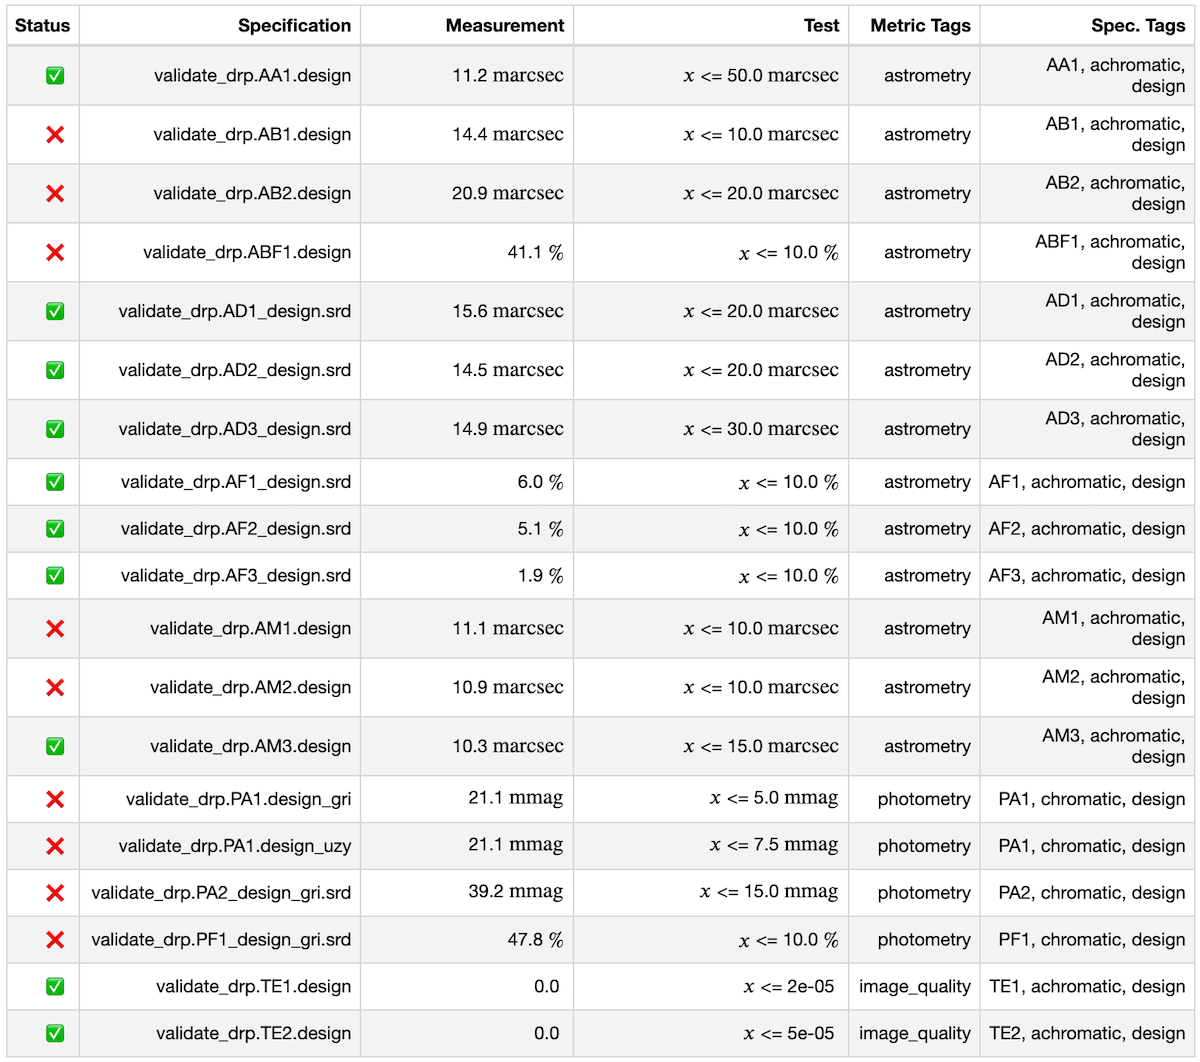
\includegraphics[width=4.31250in]{jira_imgs/1297.png}

\medskip }
\end{minipage} \\ \cdashline{2-2}

 & Status: \textbf{ Pass } \\ \hline

\end{longtable}

\paragraph{Test Case LVV-T1746 -  Verify calculation of fraction of relative astrometric measurement error
on 5 arcminute scales exceeding outlier limit
 }\mbox{}\\

Open  \href{https://jira.lsstcorp.org/secure/Tests.jspa#/testCase/LVV-T1746}{\textit{ LVV-T1746 } }
test case in Jira.

 Verify that the DM system has provided the code to calculate the maximum
fraction of relative astrometric measurements on 5 arcminute scales that
exceed the 5 arcminute outlier limit \textbf{AD1 = 20 milliarcseconds},
and assess whether it meets the requirement that it shall be less than
\textbf{AF1 = 10 percent.}


\textbf{ Preconditions}:\\


Execution status: {\bf Pass }

Final comment:\\ Tests executed on lsst-dev, using Release v19.0.0.



Detailed steps results:

\begin{longtable}{p{1cm}p{15cm}}
\hline
{Step} & Step Details\\ \hline
1 & Description \\
 & \begin{minipage}[t]{15cm}
{\footnotesize
Identify a dataset containing at least one field with multiple
overlapping visits.

\medskip }
\end{minipage}
\\ \cdashline{2-2}


 & Expected Result \\
 & \begin{minipage}[t]{15cm}{\footnotesize
A dataset that has been ingested into a Butler repository.

\medskip }
\end{minipage} \\ \cdashline{2-2}

 & Actual Result \\
 & \begin{minipage}[t]{15cm}{\footnotesize
We used the output repo from HSC-RC2 data processing, as executed using
the weekly pipelines release (w\_2019\_46) that became v19.0.0. The
output repo is tagged with the Jira ticket number
\href{https://jira.lsstcorp.org/browse/DM-22223}{DM-22223}.\\[2\baselineskip]The
path to the dataset on the development cluster (lsst-dev) is
`/datasets/hsc/repo/rerun/RC/w\_2019\_46/DM-22223'.

\medskip }
\end{minipage} \\ \cdashline{2-2}

 & Status: \textbf{ Pass } \\ \hline

2 & Description \\
 & \begin{minipage}[t]{15cm}
{\footnotesize
The `path` that you will use depends on where you are running the
science pipelines. Options:\\[2\baselineskip]

\begin{itemize}
\tightlist
\item
  local (newinstall.sh - based
  install):{[}path\_to\_installation{]}/loadLSST.bash
\item
  development cluster (``lsst-dev''):
  /software/lsstsw/stack/loadLSST.bash
\item
  LSP Notebook aspect (from a terminal):
  /opt/lsst/software/stack/loadLSST.bash
\end{itemize}

From the command line, execute the commands below in the example
code:\\[2\baselineskip]

\medskip }
\end{minipage}
\\ \cdashline{2-2}

 & Example Code \\
 & \begin{minipage}[t]{15cm}{\footnotesize
source `path`\\
setup lsst\_distrib

\medskip }
\end{minipage} \\ \cdashline{2-2}

 & Expected Result \\
 & \begin{minipage}[t]{15cm}{\footnotesize
Science pipeline software is available for use. If additional packages
are needed (for example, `obs' packages such as `obs\_subaru`), then
additional `setup` commands will be necessary.\\[2\baselineskip]To check
versions in use, type:\\
eups list -s

\medskip }
\end{minipage} \\ \cdashline{2-2}

 & Actual Result \\
 & \begin{minipage}[t]{15cm}{\footnotesize
On lsst-dev, the setup was done as follows:\\[2\baselineskip]source
/software/lsstsw/stack/loadLSST.bash\\
source scl\_source enable devtoolset-8\\
setup -t w\_2019\_46 lsst\_distrib\\
setup obs\_subaru\\
setup validate\_drp

\medskip }
\end{minipage} \\ \cdashline{2-2}

 & Status: \textbf{ Pass } \\ \hline

3 & Description \\
 & \begin{minipage}[t]{15cm}
{\footnotesize
Execute `validate\_drp` on a repository containing precursor data.
Identify the path to the data, which we will call `DATA/path', then
execute the following (with additional flags specified as needed):

\medskip }
\end{minipage}
\\ \cdashline{2-2}

 & Example Code \\
 & \begin{minipage}[t]{15cm}{\footnotesize
validateDrp.py `DATA/path`

\medskip }
\end{minipage} \\ \cdashline{2-2}

 & Expected Result \\
 & \begin{minipage}[t]{15cm}{\footnotesize
JSON files (and associated figures) containing the Measurements and any
associated ``extras.''

\medskip }
\end{minipage} \\ \cdashline{2-2}

 & Actual Result \\
 & \begin{minipage}[t]{15cm}{\footnotesize
Batch jobs were sent to via slurm jobs to the batch processing cluster
using a script that looked like (submitted via `sbatch
SCRIPTNAME`):\\[2\baselineskip]\#!/bin/bash -l\\[2\baselineskip]\#SBATCH
-p normal\\
\#SBATCH -N 1\\
\#SBATCH --ntasks-per-node=1\\
\#SBATCH -t 18:00:00\\
\#SBATCH -J v9697\\
\#SBATCH
--output=/project/jcarlin/verify/RC2\_v3/validateDrp/logs/rc2-9697-\%j.log\\
\#SBATCH
--error=/project/jcarlin/verify/RC2\_v3/validateDrp/logs/rc2-9697-\%j.log\\[2\baselineskip]srun
validateDrp.py /datasets/hsc/repo/rerun/RC/w\_2019\_46/DM-22223
--configFile `cfg9697\_all.yaml'
--outputPrefix='tract9697'\\[2\baselineskip]\ldots{}where the
configuration file (cfg9697\_all.yaml) contained something like
this:\\[2\baselineskip]\# Configuration information for validate\_drp
to\\
\# build the list of data IDs to analyze\\
tracts: {[}9697{]}\\
visits:
{[}6320,34338,34342,34362,34366,34382,34384,34400,34402,34412,34414,34422,34424,34448,34450,34464,34468,34478,34480,34482,34484,34486,35870,35890,35892,35906,35936,35950,35974,36114,36118,36140,36144,36148,36158,36160,36170,36172,36180,36182,36190,36192,36202,36204,36212,36214,36216,36218,36234,36236,36238,36240,36258,36260,36262,7138,34640,34644,34648,34652,34664,34670,34672,34674,34676,34686,34688,34690,34698,34706,34708,34712,34714,34734,34758,34760,34772,34874,34942,34944,34946,36726,36730,36738,36750,36754,36756,36758,36762,36768,36772,36774,36776,36778,36788,36790,36792,36794,36800,36802,36808,36810,36812,36818,36820,36828,36830,36834,36836,36838,36404,36408,36412,36416,36424,36426,36428,36430,36432,36434,36438,36442,36444,36446,36448,36456,36458,36460,36466,36474,36476,36480,36488,36490,36492,36494,36498,36504,36506,36508,38938,38944,38950{]}\\
filter:
{[}'HSC-G','HSC-G','HSC-G','HSC-G','HSC-G','HSC-G','HSC-G','HSC-G','HSC-G','HSC-G','HSC-G','HSC-G','HSC-G','HSC-G','HSC-G','HSC-G','HSC-G','HSC-G','HSC-G','HSC-G','HSC-G','HSC-G','HSC-I','HSC-I','HSC-I','HSC-I','HSC-I','HSC-I','HSC-I','HSC-I','HSC-I','HSC-I','HSC-I','HSC-I','HSC-I','HSC-I','HSC-I','HSC-I','HSC-I','HSC-I','HSC-I','HSC-I','HSC-I','HSC-I','HSC-I','HSC-I','HSC-I','HSC-I','HSC-I','HSC-I','HSC-I','HSC-I','HSC-I','HSC-I','HSC-I','HSC-R','HSC-R','HSC-R','HSC-R','HSC-R','HSC-R','HSC-R','HSC-R','HSC-R','HSC-R','HSC-R','HSC-R','HSC-R','HSC-R','HSC-R','HSC-R','HSC-R','HSC-R','HSC-R','HSC-R','HSC-R','HSC-R','HSC-Y','HSC-Y','HSC-Y','HSC-Y','HSC-Y','HSC-Y','HSC-Y','HSC-Y','HSC-Y','HSC-Y','HSC-Y','HSC-Y','HSC-Y','HSC-Y','HSC-Y','HSC-Y','HSC-Y','HSC-Y','HSC-Y','HSC-Y','HSC-Y','HSC-Y','HSC-Y','HSC-Y','HSC-Y','HSC-Y','HSC-Y','HSC-Y','HSC-Y','HSC-Y','HSC-Y','HSC-Y','HSC-Y','HSC-Z','HSC-Z','HSC-Z','HSC-Z','HSC-Z','HSC-Z','HSC-Z','HSC-Z','HSC-Z','HSC-Z','HSC-Z','HSC-Z','HSC-Z','HSC-Z','HSC-Z','HSC-Z','HSC-Z','HSC-Z','HSC-Z','HSC-Z','HSC-Z','HSC-Z','HSC-Z','HSC-Z','HSC-Z','HSC-Z','HSC-Z','HSC-Z','HSC-Z','HSC-Z','HSC-Z','HSC-Z','HSC-Z'{]}\\
ccd: {[}0, 1, 2, 3, 4, 5, 6, 7, 8, 10, 11, 12, 13, 14, 15, 16, 17, 18,
19, 20, 21, 22, 23, 24, 25, 26, 27, 28, 29, 30, 31, 32, 33, 34, 35, 36,
37, 38, 39, 40, 41, 42, 43, 44, 45, 46, 47, 48, 49, 50, 51, 52, 53, 54,
55, 56, 57, 58, 59, 60, 61, 62, 63, 64, 65, 66, 67, 68, 69, 70, 71, 72,
73, 74, 75, 76, 77, 78, 79, 80, 81, 82, 83, 84, 85, 86, 87, 88, 89, 90,
91, 92, 93, 94, 95, 96, 97, 98, 99, 100, 101, 102, 103{]}\\
instrument: `HSC'\\[2\baselineskip]

\medskip }
\end{minipage} \\ \cdashline{2-2}

 & Status: \textbf{ Pass } \\ \hline

4 & Description \\
 & \begin{minipage}[t]{15cm}
{\footnotesize
Confirm that the metric AF1 has been calculated using the outlier limit
AD1, and that its values are reasonable.

\medskip }
\end{minipage}
\\ \cdashline{2-2}


 & Expected Result \\
 & \begin{minipage}[t]{15cm}{\footnotesize
A JSON file (and/or a report generated from that JSON file)
demonstrating that AF1 has been calculated (and used the limit AD1).

\medskip }
\end{minipage} \\ \cdashline{2-2}

 & Actual Result \\
 & \begin{minipage}[t]{15cm}{\footnotesize
This was confirmed by

\begin{enumerate}
\def\labelenumi{\alph{enumi}.}
\tightlist
\item
  loading the JSON and printing a report from within a Jupyterlab
  notebook on the LSP (see attached rendering of notebook; the notebook
  is saved in as `test\_KPMs\_validate\_drp.ipynb` in the DMTR-201
  github repository), and~
\item
  dispatching the metric measurements to the SQuaSH chronograf dashboard
  (see attached screen shot).\\[2\baselineskip]
\end{enumerate}

See the documents attached to LVV-T1745 for illustration of the
results.\\[2\baselineskip]The adopted value for AD1 was verified by
inspecting the validate\_drp source code. Note that AD1 is also
calculated in validate\_drp as the value of the residual at the 10th
percentile (i.e., the design value of AF1).\\[2\baselineskip]The
calculated value of AF1 for the example case (tract 9615, HSC-I filter)
illustrated in the attached document is AF1 = 6.0\%, which is near the
design threshold of 10.0\%.

\medskip }
\end{minipage} \\ \cdashline{2-2}

 & Status: \textbf{ Pass } \\ \hline

\end{longtable}

\paragraph{Test Case LVV-T1747 -  Verify calculation of relative astrometric measurement error on 5
arcminute scales
 }\mbox{}\\

Open  \href{https://jira.lsstcorp.org/secure/Tests.jspa#/testCase/LVV-T1747}{\textit{ LVV-T1747 } }
test case in Jira.

 Verify that the DM system has provided the code to calculate the
relative astrometric measurement error on 5 arcminute scales, and assess
whether it meets the requirement that it shall be less
than\textbf{~\textbf{AM1 = 10 milliarcseconds.}}


\textbf{ Preconditions}:\\


Execution status: {\bf Pass }

Final comment:\\ Tests executed on lsst-dev, using Release v19.0.0.



Detailed steps results:

\begin{longtable}{p{1cm}p{15cm}}
\hline
{Step} & Step Details\\ \hline
1 & Description \\
 & \begin{minipage}[t]{15cm}
{\footnotesize
Identify a dataset containing at least one field with multiple
overlapping visits.

\medskip }
\end{minipage}
\\ \cdashline{2-2}


 & Expected Result \\
 & \begin{minipage}[t]{15cm}{\footnotesize
A dataset that has been ingested into a Butler repository.

\medskip }
\end{minipage} \\ \cdashline{2-2}

 & Actual Result \\
 & \begin{minipage}[t]{15cm}{\footnotesize
We used the output repo from HSC-RC2 data processing, as executed using
the weekly pipelines release (w\_2019\_46) that became v19.0.0. The
output repo is tagged with the Jira ticket number
\href{https://jira.lsstcorp.org/browse/DM-22223}{DM-22223}.\\[2\baselineskip]The
path to the dataset on the development cluster (lsst-dev) is
`/datasets/hsc/repo/rerun/RC/w\_2019\_46/DM-22223'.

\medskip }
\end{minipage} \\ \cdashline{2-2}

 & Status: \textbf{ Pass } \\ \hline

2 & Description \\
 & \begin{minipage}[t]{15cm}
{\footnotesize
The `path` that you will use depends on where you are running the
science pipelines. Options:\\[2\baselineskip]

\begin{itemize}
\tightlist
\item
  local (newinstall.sh - based
  install):{[}path\_to\_installation{]}/loadLSST.bash
\item
  development cluster (``lsst-dev''):
  /software/lsstsw/stack/loadLSST.bash
\item
  LSP Notebook aspect (from a terminal):
  /opt/lsst/software/stack/loadLSST.bash
\end{itemize}

From the command line, execute the commands below in the example
code:\\[2\baselineskip]

\medskip }
\end{minipage}
\\ \cdashline{2-2}

 & Example Code \\
 & \begin{minipage}[t]{15cm}{\footnotesize
source `path`\\
setup lsst\_distrib

\medskip }
\end{minipage} \\ \cdashline{2-2}

 & Expected Result \\
 & \begin{minipage}[t]{15cm}{\footnotesize
Science pipeline software is available for use. If additional packages
are needed (for example, `obs' packages such as `obs\_subaru`), then
additional `setup` commands will be necessary.\\[2\baselineskip]To check
versions in use, type:\\
eups list -s

\medskip }
\end{minipage} \\ \cdashline{2-2}

 & Actual Result \\
 & \begin{minipage}[t]{15cm}{\footnotesize

\medskip }
\end{minipage} \\ \cdashline{2-2}

 & Status: \textbf{ Not Executed } \\ \hline

3 & Description \\
 & \begin{minipage}[t]{15cm}
{\footnotesize
Execute `validate\_drp` on a repository containing precursor data.
Identify the path to the data, which we will call `DATA/path', then
execute the following (with additional flags specified as needed):

\medskip }
\end{minipage}
\\ \cdashline{2-2}

 & Example Code \\
 & \begin{minipage}[t]{15cm}{\footnotesize
validateDrp.py `DATA/path`

\medskip }
\end{minipage} \\ \cdashline{2-2}

 & Expected Result \\
 & \begin{minipage}[t]{15cm}{\footnotesize
JSON files (and associated figures) containing the Measurements and any
associated ``extras.''

\medskip }
\end{minipage} \\ \cdashline{2-2}

 & Actual Result \\
 & \begin{minipage}[t]{15cm}{\footnotesize
Batch jobs were sent to via slurm jobs to the batch processing cluster
using a script that looked like (submitted via `sbatch
SCRIPTNAME`):\\[2\baselineskip]\#!/bin/bash -l\\[2\baselineskip]\#SBATCH
-p normal\\
\#SBATCH -N 1\\
\#SBATCH --ntasks-per-node=1\\
\#SBATCH -t 18:00:00\\
\#SBATCH -J v9697\\
\#SBATCH
--output=/project/jcarlin/verify/RC2\_v3/validateDrp/logs/rc2-9697-\%j.log\\
\#SBATCH
--error=/project/jcarlin/verify/RC2\_v3/validateDrp/logs/rc2-9697-\%j.log\\[2\baselineskip]srun
validateDrp.py /datasets/hsc/repo/rerun/RC/w\_2019\_46/DM-22223
--configFile `cfg9697\_all.yaml'
--outputPrefix='tract9697'\\[2\baselineskip]\ldots{}where the
configuration file (cfg9697\_all.yaml) contained something like
this:\\[2\baselineskip]\# Configuration information for validate\_drp
to\\
\# build the list of data IDs to analyze\\
tracts: {[}9697{]}\\
visits:
{[}6320,34338,34342,34362,34366,34382,34384,34400,34402,34412,34414,34422,34424,34448,34450,34464,34468,34478,34480,34482,34484,34486,35870,35890,35892,35906,35936,35950,35974,36114,36118,36140,36144,36148,36158,36160,36170,36172,36180,36182,36190,36192,36202,36204,36212,36214,36216,36218,36234,36236,36238,36240,36258,36260,36262,7138,34640,34644,34648,34652,34664,34670,34672,34674,34676,34686,34688,34690,34698,34706,34708,34712,34714,34734,34758,34760,34772,34874,34942,34944,34946,36726,36730,36738,36750,36754,36756,36758,36762,36768,36772,36774,36776,36778,36788,36790,36792,36794,36800,36802,36808,36810,36812,36818,36820,36828,36830,36834,36836,36838,36404,36408,36412,36416,36424,36426,36428,36430,36432,36434,36438,36442,36444,36446,36448,36456,36458,36460,36466,36474,36476,36480,36488,36490,36492,36494,36498,36504,36506,36508,38938,38944,38950{]}\\
filter:
{[}'HSC-G','HSC-G','HSC-G','HSC-G','HSC-G','HSC-G','HSC-G','HSC-G','HSC-G','HSC-G','HSC-G','HSC-G','HSC-G','HSC-G','HSC-G','HSC-G','HSC-G','HSC-G','HSC-G','HSC-G','HSC-G','HSC-G','HSC-I','HSC-I','HSC-I','HSC-I','HSC-I','HSC-I','HSC-I','HSC-I','HSC-I','HSC-I','HSC-I','HSC-I','HSC-I','HSC-I','HSC-I','HSC-I','HSC-I','HSC-I','HSC-I','HSC-I','HSC-I','HSC-I','HSC-I','HSC-I','HSC-I','HSC-I','HSC-I','HSC-I','HSC-I','HSC-I','HSC-I','HSC-I','HSC-I','HSC-R','HSC-R','HSC-R','HSC-R','HSC-R','HSC-R','HSC-R','HSC-R','HSC-R','HSC-R','HSC-R','HSC-R','HSC-R','HSC-R','HSC-R','HSC-R','HSC-R','HSC-R','HSC-R','HSC-R','HSC-R','HSC-R','HSC-Y','HSC-Y','HSC-Y','HSC-Y','HSC-Y','HSC-Y','HSC-Y','HSC-Y','HSC-Y','HSC-Y','HSC-Y','HSC-Y','HSC-Y','HSC-Y','HSC-Y','HSC-Y','HSC-Y','HSC-Y','HSC-Y','HSC-Y','HSC-Y','HSC-Y','HSC-Y','HSC-Y','HSC-Y','HSC-Y','HSC-Y','HSC-Y','HSC-Y','HSC-Y','HSC-Y','HSC-Y','HSC-Y','HSC-Z','HSC-Z','HSC-Z','HSC-Z','HSC-Z','HSC-Z','HSC-Z','HSC-Z','HSC-Z','HSC-Z','HSC-Z','HSC-Z','HSC-Z','HSC-Z','HSC-Z','HSC-Z','HSC-Z','HSC-Z','HSC-Z','HSC-Z','HSC-Z','HSC-Z','HSC-Z','HSC-Z','HSC-Z','HSC-Z','HSC-Z','HSC-Z','HSC-Z','HSC-Z','HSC-Z','HSC-Z','HSC-Z'{]}\\
ccd: {[}0, 1, 2, 3, 4, 5, 6, 7, 8, 10, 11, 12, 13, 14, 15, 16, 17, 18,
19, 20, 21, 22, 23, 24, 25, 26, 27, 28, 29, 30, 31, 32, 33, 34, 35, 36,
37, 38, 39, 40, 41, 42, 43, 44, 45, 46, 47, 48, 49, 50, 51, 52, 53, 54,
55, 56, 57, 58, 59, 60, 61, 62, 63, 64, 65, 66, 67, 68, 69, 70, 71, 72,
73, 74, 75, 76, 77, 78, 79, 80, 81, 82, 83, 84, 85, 86, 87, 88, 89, 90,
91, 92, 93, 94, 95, 96, 97, 98, 99, 100, 101, 102, 103{]}\\
instrument: `HSC'\\[2\baselineskip]

\medskip }
\end{minipage} \\ \cdashline{2-2}

 & Status: \textbf{ Pass } \\ \hline

4 & Description \\
 & \begin{minipage}[t]{15cm}
{\footnotesize
Confirm that the metric AM1 has been calculated, and that its values are
reasonable.

\medskip }
\end{minipage}
\\ \cdashline{2-2}


 & Expected Result \\
 & \begin{minipage}[t]{15cm}{\footnotesize
A JSON file (and/or a report generated from that JSON file)
demonstrating that AM1 has been calculated.

\medskip }
\end{minipage} \\ \cdashline{2-2}

 & Actual Result \\
 & \begin{minipage}[t]{15cm}{\footnotesize
This was confirmed by

\begin{enumerate}
\def\labelenumi{\alph{enumi}.}
\tightlist
\item
  loading the JSON and printing a report from within a Jupyterlab
  notebook on the LSP (see attached rendering of notebook; the notebook
  is saved in as `test\_KPMs\_validate\_drp.ipynb` in the DMTR-201
  github repository), and~
\item
  dispatching the metric measurements to the SQuaSH chronograf dashboard
  (see attached screen shot).\\[2\baselineskip]
\end{enumerate}

See the documents attached to LVV-T1745 for illustration of the
results.\\[2\baselineskip]The calculated value of AM1 for the example
case (tract 9615, HSC-I filter) illustrated in the attached document is
AM1 = 11.1 mas, which is near the design threshold of 10.0 mas.

\medskip }
\end{minipage} \\ \cdashline{2-2}

 & Status: \textbf{ Pass } \\ \hline

\end{longtable}

\paragraph{Test Case LVV-T1748 -  Verify calculation of median error in absolute position for RA, Dec axes
 }\mbox{}\\

Open  \href{https://jira.lsstcorp.org/secure/Tests.jspa#/testCase/LVV-T1748}{\textit{ LVV-T1748 } }
test case in Jira.

 Verify that the DM system has provided the code to calculate the median
error in absolute position for each axis, RA and DEC, and assess whether
it meets the requirement that it shall be less than \textbf{AA1 = 50
milliarcseconds}.


\textbf{ Preconditions}:\\


Execution status: {\bf Pass }

Final comment:\\ Tests executed on lsst-dev, using Release v19.0.0.



Detailed steps results:

\begin{longtable}{p{1cm}p{15cm}}
\hline
{Step} & Step Details\\ \hline
1 & Description \\
 & \begin{minipage}[t]{15cm}
{\footnotesize
Identify a dataset containing at least one field with multiple
overlapping visits.

\medskip }
\end{minipage}
\\ \cdashline{2-2}


 & Expected Result \\
 & \begin{minipage}[t]{15cm}{\footnotesize
A dataset that has been ingested into a Butler repository.

\medskip }
\end{minipage} \\ \cdashline{2-2}

 & Actual Result \\
 & \begin{minipage}[t]{15cm}{\footnotesize
We used the output repo from HSC-RC2 data processing, as executed using
the weekly pipelines release (w\_2019\_46) that became v19.0.0. The
output repo is tagged with the Jira ticket number
\href{https://jira.lsstcorp.org/browse/DM-22223}{DM-22223}.\\[2\baselineskip]The
path to the dataset on the development cluster (lsst-dev) is
`/datasets/hsc/repo/rerun/RC/w\_2019\_46/DM-22223'.

\medskip }
\end{minipage} \\ \cdashline{2-2}

 & Status: \textbf{ Pass } \\ \hline

2 & Description \\
 & \begin{minipage}[t]{15cm}
{\footnotesize
The `path` that you will use depends on where you are running the
science pipelines. Options:\\[2\baselineskip]

\begin{itemize}
\tightlist
\item
  local (newinstall.sh - based
  install):{[}path\_to\_installation{]}/loadLSST.bash
\item
  development cluster (``lsst-dev''):
  /software/lsstsw/stack/loadLSST.bash
\item
  LSP Notebook aspect (from a terminal):
  /opt/lsst/software/stack/loadLSST.bash
\end{itemize}

From the command line, execute the commands below in the example
code:\\[2\baselineskip]

\medskip }
\end{minipage}
\\ \cdashline{2-2}

 & Example Code \\
 & \begin{minipage}[t]{15cm}{\footnotesize
source `path`\\
setup lsst\_distrib

\medskip }
\end{minipage} \\ \cdashline{2-2}

 & Expected Result \\
 & \begin{minipage}[t]{15cm}{\footnotesize
Science pipeline software is available for use. If additional packages
are needed (for example, `obs' packages such as `obs\_subaru`), then
additional `setup` commands will be necessary.\\[2\baselineskip]To check
versions in use, type:\\
eups list -s

\medskip }
\end{minipage} \\ \cdashline{2-2}

 & Actual Result \\
 & \begin{minipage}[t]{15cm}{\footnotesize
On lsst-dev, the setup was done as follows:\\[2\baselineskip]source
/software/lsstsw/stack/loadLSST.bash\\
source scl\_source enable devtoolset-8\\
setup -t w\_2019\_46 lsst\_distrib\\
setup obs\_subaru\\
setup validate\_drp

\medskip }
\end{minipage} \\ \cdashline{2-2}

 & Status: \textbf{ Pass } \\ \hline

3 & Description \\
 & \begin{minipage}[t]{15cm}
{\footnotesize
Execute `validate\_drp` on a repository containing precursor data.
Identify the path to the data, which we will call `DATA/path', then
execute the following (with additional flags specified as needed):

\medskip }
\end{minipage}
\\ \cdashline{2-2}

 & Example Code \\
 & \begin{minipage}[t]{15cm}{\footnotesize
validateDrp.py `DATA/path`

\medskip }
\end{minipage} \\ \cdashline{2-2}

 & Expected Result \\
 & \begin{minipage}[t]{15cm}{\footnotesize
JSON files (and associated figures) containing the Measurements and any
associated ``extras.''

\medskip }
\end{minipage} \\ \cdashline{2-2}

 & Actual Result \\
 & \begin{minipage}[t]{15cm}{\footnotesize
Batch jobs were sent to via slurm jobs to the batch processing cluster
using a script that looked like (submitted via `sbatch
SCRIPTNAME`):\\[2\baselineskip]\#!/bin/bash -l\\[2\baselineskip]\#SBATCH
-p normal\\
\#SBATCH -N 1\\
\#SBATCH --ntasks-per-node=1\\
\#SBATCH -t 18:00:00\\
\#SBATCH -J v9697\\
\#SBATCH
--output=/project/jcarlin/verify/RC2\_v3/validateDrp/logs/rc2-9697-\%j.log\\
\#SBATCH
--error=/project/jcarlin/verify/RC2\_v3/validateDrp/logs/rc2-9697-\%j.log\\[2\baselineskip]srun
validateDrp.py /datasets/hsc/repo/rerun/RC/w\_2019\_46/DM-22223
--configFile `cfg9697\_all.yaml'
--outputPrefix='tract9697'\\[2\baselineskip]\ldots{}where the
configuration file (cfg9697\_all.yaml) contained something like
this:\\[2\baselineskip]\# Configuration information for validate\_drp
to\\
\# build the list of data IDs to analyze\\
tracts: {[}9697{]}\\
visits:
{[}6320,34338,34342,34362,34366,34382,34384,34400,34402,34412,34414,34422,34424,34448,34450,34464,34468,34478,34480,34482,34484,34486,35870,35890,35892,35906,35936,35950,35974,36114,36118,36140,36144,36148,36158,36160,36170,36172,36180,36182,36190,36192,36202,36204,36212,36214,36216,36218,36234,36236,36238,36240,36258,36260,36262,7138,34640,34644,34648,34652,34664,34670,34672,34674,34676,34686,34688,34690,34698,34706,34708,34712,34714,34734,34758,34760,34772,34874,34942,34944,34946,36726,36730,36738,36750,36754,36756,36758,36762,36768,36772,36774,36776,36778,36788,36790,36792,36794,36800,36802,36808,36810,36812,36818,36820,36828,36830,36834,36836,36838,36404,36408,36412,36416,36424,36426,36428,36430,36432,36434,36438,36442,36444,36446,36448,36456,36458,36460,36466,36474,36476,36480,36488,36490,36492,36494,36498,36504,36506,36508,38938,38944,38950{]}\\
filter:
{[}'HSC-G','HSC-G','HSC-G','HSC-G','HSC-G','HSC-G','HSC-G','HSC-G','HSC-G','HSC-G','HSC-G','HSC-G','HSC-G','HSC-G','HSC-G','HSC-G','HSC-G','HSC-G','HSC-G','HSC-G','HSC-G','HSC-G','HSC-I','HSC-I','HSC-I','HSC-I','HSC-I','HSC-I','HSC-I','HSC-I','HSC-I','HSC-I','HSC-I','HSC-I','HSC-I','HSC-I','HSC-I','HSC-I','HSC-I','HSC-I','HSC-I','HSC-I','HSC-I','HSC-I','HSC-I','HSC-I','HSC-I','HSC-I','HSC-I','HSC-I','HSC-I','HSC-I','HSC-I','HSC-I','HSC-I','HSC-R','HSC-R','HSC-R','HSC-R','HSC-R','HSC-R','HSC-R','HSC-R','HSC-R','HSC-R','HSC-R','HSC-R','HSC-R','HSC-R','HSC-R','HSC-R','HSC-R','HSC-R','HSC-R','HSC-R','HSC-R','HSC-R','HSC-Y','HSC-Y','HSC-Y','HSC-Y','HSC-Y','HSC-Y','HSC-Y','HSC-Y','HSC-Y','HSC-Y','HSC-Y','HSC-Y','HSC-Y','HSC-Y','HSC-Y','HSC-Y','HSC-Y','HSC-Y','HSC-Y','HSC-Y','HSC-Y','HSC-Y','HSC-Y','HSC-Y','HSC-Y','HSC-Y','HSC-Y','HSC-Y','HSC-Y','HSC-Y','HSC-Y','HSC-Y','HSC-Y','HSC-Z','HSC-Z','HSC-Z','HSC-Z','HSC-Z','HSC-Z','HSC-Z','HSC-Z','HSC-Z','HSC-Z','HSC-Z','HSC-Z','HSC-Z','HSC-Z','HSC-Z','HSC-Z','HSC-Z','HSC-Z','HSC-Z','HSC-Z','HSC-Z','HSC-Z','HSC-Z','HSC-Z','HSC-Z','HSC-Z','HSC-Z','HSC-Z','HSC-Z','HSC-Z','HSC-Z','HSC-Z','HSC-Z'{]}\\
ccd: {[}0, 1, 2, 3, 4, 5, 6, 7, 8, 10, 11, 12, 13, 14, 15, 16, 17, 18,
19, 20, 21, 22, 23, 24, 25, 26, 27, 28, 29, 30, 31, 32, 33, 34, 35, 36,
37, 38, 39, 40, 41, 42, 43, 44, 45, 46, 47, 48, 49, 50, 51, 52, 53, 54,
55, 56, 57, 58, 59, 60, 61, 62, 63, 64, 65, 66, 67, 68, 69, 70, 71, 72,
73, 74, 75, 76, 77, 78, 79, 80, 81, 82, 83, 84, 85, 86, 87, 88, 89, 90,
91, 92, 93, 94, 95, 96, 97, 98, 99, 100, 101, 102, 103{]}\\
instrument: `HSC'\\[2\baselineskip]

\medskip }
\end{minipage} \\ \cdashline{2-2}

 & Status: \textbf{ Pass } \\ \hline

4 & Description \\
 & \begin{minipage}[t]{15cm}
{\footnotesize
Confirm that the metric AA1 has been calculated, and that its values are
reasonable.

\medskip }
\end{minipage}
\\ \cdashline{2-2}


 & Expected Result \\
 & \begin{minipage}[t]{15cm}{\footnotesize
A JSON file (and/or a report generated from that JSON file)
demonstrating that AA1 has been calculated.

\medskip }
\end{minipage} \\ \cdashline{2-2}

 & Actual Result \\
 & \begin{minipage}[t]{15cm}{\footnotesize
This was confirmed by

\begin{enumerate}
\def\labelenumi{\alph{enumi}.}
\tightlist
\item
  loading the JSON and printing a report from within a Jupyterlab
  notebook on the LSP (see attached rendering of notebook; the notebook
  is saved in as `test\_KPMs\_validate\_drp.ipynb` in the DMTR-201
  github repository), and~
\item
  dispatching the metric measurements to the SQuaSH chronograf dashboard
  (see attached screen shot).\\[2\baselineskip]
\end{enumerate}

See the documents attached to LVV-T1745 for illustration of the
results.\\[2\baselineskip]The calculated value of AA1 for the example
case (tract 9615, HSC-I filter) illustrated in the attached document is
AA1 = 11.2 mas, which is well below the design threshold of 50.0 mas.

\medskip }
\end{minipage} \\ \cdashline{2-2}

 & Status: \textbf{ Pass } \\ \hline

\end{longtable}

\paragraph{Test Case LVV-T1749 -  Verify calculation of fraction of relative astrometric measurement error
on 20 arcminute scales exceeding outlier limit
 }\mbox{}\\

Open  \href{https://jira.lsstcorp.org/secure/Tests.jspa#/testCase/LVV-T1749}{\textit{ LVV-T1749 } }
test case in Jira.

 Verify that the DM system has provided the code to calculate the maximum
fraction of relative astrometric measurements on 20 arcminute scales
that exceed the 20 arcminute outlier limit \textbf{AD2 = 20
milliarcseconds}, and assess whether it meets the requirement that it
shall be less than \textbf{AF2 = 10 percent.}


\textbf{ Preconditions}:\\


Execution status: {\bf Pass }

Final comment:\\ Tests executed on lsst-dev, using Release v19.0.0.



Detailed steps results:

\begin{longtable}{p{1cm}p{15cm}}
\hline
{Step} & Step Details\\ \hline
1 & Description \\
 & \begin{minipage}[t]{15cm}
{\footnotesize
Identify a dataset containing at least one field with multiple
overlapping visits.

\medskip }
\end{minipage}
\\ \cdashline{2-2}


 & Expected Result \\
 & \begin{minipage}[t]{15cm}{\footnotesize
A dataset that has been ingested into a Butler repository.

\medskip }
\end{minipage} \\ \cdashline{2-2}

 & Actual Result \\
 & \begin{minipage}[t]{15cm}{\footnotesize
We used the output repo from HSC-RC2 data processing, as executed using
the weekly pipelines release (w\_2019\_46) that became v19.0.0. The
output repo is tagged with the Jira ticket number
\href{https://jira.lsstcorp.org/browse/DM-22223}{DM-22223}.\\[2\baselineskip]The
path to the dataset on the development cluster (lsst-dev) is
`/datasets/hsc/repo/rerun/RC/w\_2019\_46/DM-22223'.

\medskip }
\end{minipage} \\ \cdashline{2-2}

 & Status: \textbf{ Pass } \\ \hline

2 & Description \\
 & \begin{minipage}[t]{15cm}
{\footnotesize
The `path` that you will use depends on where you are running the
science pipelines. Options:\\[2\baselineskip]

\begin{itemize}
\tightlist
\item
  local (newinstall.sh - based
  install):{[}path\_to\_installation{]}/loadLSST.bash
\item
  development cluster (``lsst-dev''):
  /software/lsstsw/stack/loadLSST.bash
\item
  LSP Notebook aspect (from a terminal):
  /opt/lsst/software/stack/loadLSST.bash
\end{itemize}

From the command line, execute the commands below in the example
code:\\[2\baselineskip]

\medskip }
\end{minipage}
\\ \cdashline{2-2}

 & Example Code \\
 & \begin{minipage}[t]{15cm}{\footnotesize
source `path`\\
setup lsst\_distrib

\medskip }
\end{minipage} \\ \cdashline{2-2}

 & Expected Result \\
 & \begin{minipage}[t]{15cm}{\footnotesize
Science pipeline software is available for use. If additional packages
are needed (for example, `obs' packages such as `obs\_subaru`), then
additional `setup` commands will be necessary.\\[2\baselineskip]To check
versions in use, type:\\
eups list -s

\medskip }
\end{minipage} \\ \cdashline{2-2}

 & Actual Result \\
 & \begin{minipage}[t]{15cm}{\footnotesize
On lsst-dev, the setup was done as follows:\\[2\baselineskip]source
/software/lsstsw/stack/loadLSST.bash\\
source scl\_source enable devtoolset-8\\
setup -t w\_2019\_46 lsst\_distrib\\
setup obs\_subaru\\
setup validate\_drp

\medskip }
\end{minipage} \\ \cdashline{2-2}

 & Status: \textbf{ Pass } \\ \hline

3 & Description \\
 & \begin{minipage}[t]{15cm}
{\footnotesize
Execute `validate\_drp` on a repository containing precursor data.
Identify the path to the data, which we will call `DATA/path', then
execute the following (with additional flags specified as needed):

\medskip }
\end{minipage}
\\ \cdashline{2-2}

 & Example Code \\
 & \begin{minipage}[t]{15cm}{\footnotesize
validateDrp.py `DATA/path`

\medskip }
\end{minipage} \\ \cdashline{2-2}

 & Expected Result \\
 & \begin{minipage}[t]{15cm}{\footnotesize
JSON files (and associated figures) containing the Measurements and any
associated ``extras.''

\medskip }
\end{minipage} \\ \cdashline{2-2}

 & Actual Result \\
 & \begin{minipage}[t]{15cm}{\footnotesize
Batch jobs were sent to via slurm jobs to the batch processing cluster
using a script that looked like (submitted via `sbatch
SCRIPTNAME`):\\[2\baselineskip]\#!/bin/bash -l\\[2\baselineskip]\#SBATCH
-p normal\\
\#SBATCH -N 1\\
\#SBATCH --ntasks-per-node=1\\
\#SBATCH -t 18:00:00\\
\#SBATCH -J v9697\\
\#SBATCH
--output=/project/jcarlin/verify/RC2\_v3/validateDrp/logs/rc2-9697-\%j.log\\
\#SBATCH
--error=/project/jcarlin/verify/RC2\_v3/validateDrp/logs/rc2-9697-\%j.log\\[2\baselineskip]srun
validateDrp.py /datasets/hsc/repo/rerun/RC/w\_2019\_46/DM-22223
--configFile `cfg9697\_all.yaml'
--outputPrefix='tract9697'\\[2\baselineskip]\ldots{}where the
configuration file (cfg9697\_all.yaml) contained something like
this:\\[2\baselineskip]\# Configuration information for validate\_drp
to\\
\# build the list of data IDs to analyze\\
tracts: {[}9697{]}\\
visits:
{[}6320,34338,34342,34362,34366,34382,34384,34400,34402,34412,34414,34422,34424,34448,34450,34464,34468,34478,34480,34482,34484,34486,35870,35890,35892,35906,35936,35950,35974,36114,36118,36140,36144,36148,36158,36160,36170,36172,36180,36182,36190,36192,36202,36204,36212,36214,36216,36218,36234,36236,36238,36240,36258,36260,36262,7138,34640,34644,34648,34652,34664,34670,34672,34674,34676,34686,34688,34690,34698,34706,34708,34712,34714,34734,34758,34760,34772,34874,34942,34944,34946,36726,36730,36738,36750,36754,36756,36758,36762,36768,36772,36774,36776,36778,36788,36790,36792,36794,36800,36802,36808,36810,36812,36818,36820,36828,36830,36834,36836,36838,36404,36408,36412,36416,36424,36426,36428,36430,36432,36434,36438,36442,36444,36446,36448,36456,36458,36460,36466,36474,36476,36480,36488,36490,36492,36494,36498,36504,36506,36508,38938,38944,38950{]}\\
filter:
{[}'HSC-G','HSC-G','HSC-G','HSC-G','HSC-G','HSC-G','HSC-G','HSC-G','HSC-G','HSC-G','HSC-G','HSC-G','HSC-G','HSC-G','HSC-G','HSC-G','HSC-G','HSC-G','HSC-G','HSC-G','HSC-G','HSC-G','HSC-I','HSC-I','HSC-I','HSC-I','HSC-I','HSC-I','HSC-I','HSC-I','HSC-I','HSC-I','HSC-I','HSC-I','HSC-I','HSC-I','HSC-I','HSC-I','HSC-I','HSC-I','HSC-I','HSC-I','HSC-I','HSC-I','HSC-I','HSC-I','HSC-I','HSC-I','HSC-I','HSC-I','HSC-I','HSC-I','HSC-I','HSC-I','HSC-I','HSC-R','HSC-R','HSC-R','HSC-R','HSC-R','HSC-R','HSC-R','HSC-R','HSC-R','HSC-R','HSC-R','HSC-R','HSC-R','HSC-R','HSC-R','HSC-R','HSC-R','HSC-R','HSC-R','HSC-R','HSC-R','HSC-R','HSC-Y','HSC-Y','HSC-Y','HSC-Y','HSC-Y','HSC-Y','HSC-Y','HSC-Y','HSC-Y','HSC-Y','HSC-Y','HSC-Y','HSC-Y','HSC-Y','HSC-Y','HSC-Y','HSC-Y','HSC-Y','HSC-Y','HSC-Y','HSC-Y','HSC-Y','HSC-Y','HSC-Y','HSC-Y','HSC-Y','HSC-Y','HSC-Y','HSC-Y','HSC-Y','HSC-Y','HSC-Y','HSC-Y','HSC-Z','HSC-Z','HSC-Z','HSC-Z','HSC-Z','HSC-Z','HSC-Z','HSC-Z','HSC-Z','HSC-Z','HSC-Z','HSC-Z','HSC-Z','HSC-Z','HSC-Z','HSC-Z','HSC-Z','HSC-Z','HSC-Z','HSC-Z','HSC-Z','HSC-Z','HSC-Z','HSC-Z','HSC-Z','HSC-Z','HSC-Z','HSC-Z','HSC-Z','HSC-Z','HSC-Z','HSC-Z','HSC-Z'{]}\\
ccd: {[}0, 1, 2, 3, 4, 5, 6, 7, 8, 10, 11, 12, 13, 14, 15, 16, 17, 18,
19, 20, 21, 22, 23, 24, 25, 26, 27, 28, 29, 30, 31, 32, 33, 34, 35, 36,
37, 38, 39, 40, 41, 42, 43, 44, 45, 46, 47, 48, 49, 50, 51, 52, 53, 54,
55, 56, 57, 58, 59, 60, 61, 62, 63, 64, 65, 66, 67, 68, 69, 70, 71, 72,
73, 74, 75, 76, 77, 78, 79, 80, 81, 82, 83, 84, 85, 86, 87, 88, 89, 90,
91, 92, 93, 94, 95, 96, 97, 98, 99, 100, 101, 102, 103{]}\\
instrument: `HSC'\\[2\baselineskip]

\medskip }
\end{minipage} \\ \cdashline{2-2}

 & Status: \textbf{ Pass } \\ \hline

4 & Description \\
 & \begin{minipage}[t]{15cm}
{\footnotesize
Confirm that the metric AF2 has been calculated using the outlier limit
AD2, and that its values are reasonable.

\medskip }
\end{minipage}
\\ \cdashline{2-2}


 & Expected Result \\
 & \begin{minipage}[t]{15cm}{\footnotesize
A JSON file (and/or a report generated from that JSON file)
demonstrating that AF2 has been calculated (and used the limit AD2).

\medskip }
\end{minipage} \\ \cdashline{2-2}

 & Actual Result \\
 & \begin{minipage}[t]{15cm}{\footnotesize
This was confirmed by

\begin{enumerate}
\def\labelenumi{\alph{enumi}.}
\tightlist
\item
  loading the JSON and printing a report from within a Jupyterlab
  notebook on the LSP (see attached rendering of notebook; the notebook
  is saved in as `test\_KPMs\_validate\_drp.ipynb` in the DMTR-201
  github repository), and~
\item
  dispatching the metric measurements to the SQuaSH chronograf dashboard
  (see attached screen shot).\\[2\baselineskip]
\end{enumerate}

See the documents attached to LVV-T1745 for illustration of the
results.\\[2\baselineskip]The adopted value for AD2 was verified by
inspecting the validate\_drp source code. Note that AD2 is also
calculated in validate\_drp as the value of the residual at the 10th
percentile (i.e., the design value of AF2).\\[2\baselineskip]The
calculated value of AF2 for the example case (tract 9615, HSC-I filter)
illustrated in the attached document is AF2 = 5.1\%, which is near the
design threshold of 10.0\%.

\medskip }
\end{minipage} \\ \cdashline{2-2}

 & Status: \textbf{ Pass } \\ \hline

\end{longtable}

\paragraph{Test Case LVV-T1750 -  Verify calculation of separations relative to r-band exceeding color
difference outlier limit
 }\mbox{}\\

Open  \href{https://jira.lsstcorp.org/secure/Tests.jspa#/testCase/LVV-T1750}{\textit{ LVV-T1750 } }
test case in Jira.

 Verify that the DM system has provided the code to calculate the
separations measured relative to the r-band that exceed the color
difference outlier limit \textbf{AB2 = 20 milliarcseconds}, and assess
whether it meets the requirement that it shall be less than \textbf{ABF1
= 10 percent.~}


\textbf{ Preconditions}:\\


Execution status: {\bf Pass }

Final comment:\\ Tests executed on lsst-dev, using Release v19.0.0.



Detailed steps results:

\begin{longtable}{p{1cm}p{15cm}}
\hline
{Step} & Step Details\\ \hline
1 & Description \\
 & \begin{minipage}[t]{15cm}
{\footnotesize
Identify a dataset containing at least one field with multiple
overlapping visits, and including at least one visit in r-band.

\medskip }
\end{minipage}
\\ \cdashline{2-2}


 & Expected Result \\
 & \begin{minipage}[t]{15cm}{\footnotesize
A dataset that has been ingested into a Butler repository.

\medskip }
\end{minipage} \\ \cdashline{2-2}

 & Actual Result \\
 & \begin{minipage}[t]{15cm}{\footnotesize
We used the output repo from HSC-RC2 data processing, as executed using
the weekly pipelines release (w\_2019\_46) that became v19.0.0. The
output repo is tagged with the Jira ticket number
\href{https://jira.lsstcorp.org/browse/DM-22223}{DM-22223}.\\[2\baselineskip]The
path to the dataset on the development cluster (lsst-dev) is
`/datasets/hsc/repo/rerun/RC/w\_2019\_46/DM-22223'.

\medskip }
\end{minipage} \\ \cdashline{2-2}

 & Status: \textbf{ Pass } \\ \hline

2 & Description \\
 & \begin{minipage}[t]{15cm}
{\footnotesize
The `path` that you will use depends on where you are running the
science pipelines. Options:\\[2\baselineskip]

\begin{itemize}
\tightlist
\item
  local (newinstall.sh - based
  install):{[}path\_to\_installation{]}/loadLSST.bash
\item
  development cluster (``lsst-dev''):
  /software/lsstsw/stack/loadLSST.bash
\item
  LSP Notebook aspect (from a terminal):
  /opt/lsst/software/stack/loadLSST.bash
\end{itemize}

From the command line, execute the commands below in the example
code:\\[2\baselineskip]

\medskip }
\end{minipage}
\\ \cdashline{2-2}

 & Example Code \\
 & \begin{minipage}[t]{15cm}{\footnotesize
source `path`\\
setup lsst\_distrib

\medskip }
\end{minipage} \\ \cdashline{2-2}

 & Expected Result \\
 & \begin{minipage}[t]{15cm}{\footnotesize
Science pipeline software is available for use. If additional packages
are needed (for example, `obs' packages such as `obs\_subaru`), then
additional `setup` commands will be necessary.\\[2\baselineskip]To check
versions in use, type:\\
eups list -s

\medskip }
\end{minipage} \\ \cdashline{2-2}

 & Actual Result \\
 & \begin{minipage}[t]{15cm}{\footnotesize
On lsst-dev, the setup was done as follows:\\[2\baselineskip]source
/software/lsstsw/stack/loadLSST.bash\\
source scl\_source enable devtoolset-8\\
setup -t w\_2019\_46 lsst\_distrib\\
setup obs\_subaru\\
setup validate\_drp

\medskip }
\end{minipage} \\ \cdashline{2-2}

 & Status: \textbf{ Pass } \\ \hline

3 & Description \\
 & \begin{minipage}[t]{15cm}
{\footnotesize
Execute `validate\_drp` on a repository containing precursor data.
Identify the path to the data, which we will call `DATA/path', then
execute the following (with additional flags specified as needed):

\medskip }
\end{minipage}
\\ \cdashline{2-2}

 & Example Code \\
 & \begin{minipage}[t]{15cm}{\footnotesize
validateDrp.py `DATA/path`

\medskip }
\end{minipage} \\ \cdashline{2-2}

 & Expected Result \\
 & \begin{minipage}[t]{15cm}{\footnotesize
JSON files (and associated figures) containing the Measurements and any
associated ``extras.''

\medskip }
\end{minipage} \\ \cdashline{2-2}

 & Actual Result \\
 & \begin{minipage}[t]{15cm}{\footnotesize
Batch jobs were sent to via slurm jobs to the batch processing cluster
using a script that looked like (submitted via `sbatch
SCRIPTNAME`):\\[2\baselineskip]\#!/bin/bash -l\\[2\baselineskip]\#SBATCH
-p normal\\
\#SBATCH -N 1\\
\#SBATCH --ntasks-per-node=1\\
\#SBATCH -t 18:00:00\\
\#SBATCH -J v9697\\
\#SBATCH
--output=/project/jcarlin/verify/RC2\_v3/validateDrp/logs/rc2-9697-\%j.log\\
\#SBATCH
--error=/project/jcarlin/verify/RC2\_v3/validateDrp/logs/rc2-9697-\%j.log\\[2\baselineskip]srun
validateDrp.py /datasets/hsc/repo/rerun/RC/w\_2019\_46/DM-22223
--configFile `cfg9697\_all.yaml'
--outputPrefix='tract9697'\\[2\baselineskip]\ldots{}where the
configuration file (cfg9697\_all.yaml) contained something like
this:\\[2\baselineskip]\# Configuration information for validate\_drp
to\\
\# build the list of data IDs to analyze\\
tracts: {[}9697{]}\\
visits:
{[}6320,34338,34342,34362,34366,34382,34384,34400,34402,34412,34414,34422,34424,34448,34450,34464,34468,34478,34480,34482,34484,34486,35870,35890,35892,35906,35936,35950,35974,36114,36118,36140,36144,36148,36158,36160,36170,36172,36180,36182,36190,36192,36202,36204,36212,36214,36216,36218,36234,36236,36238,36240,36258,36260,36262,7138,34640,34644,34648,34652,34664,34670,34672,34674,34676,34686,34688,34690,34698,34706,34708,34712,34714,34734,34758,34760,34772,34874,34942,34944,34946,36726,36730,36738,36750,36754,36756,36758,36762,36768,36772,36774,36776,36778,36788,36790,36792,36794,36800,36802,36808,36810,36812,36818,36820,36828,36830,36834,36836,36838,36404,36408,36412,36416,36424,36426,36428,36430,36432,36434,36438,36442,36444,36446,36448,36456,36458,36460,36466,36474,36476,36480,36488,36490,36492,36494,36498,36504,36506,36508,38938,38944,38950{]}\\
filter:
{[}'HSC-G','HSC-G','HSC-G','HSC-G','HSC-G','HSC-G','HSC-G','HSC-G','HSC-G','HSC-G','HSC-G','HSC-G','HSC-G','HSC-G','HSC-G','HSC-G','HSC-G','HSC-G','HSC-G','HSC-G','HSC-G','HSC-G','HSC-I','HSC-I','HSC-I','HSC-I','HSC-I','HSC-I','HSC-I','HSC-I','HSC-I','HSC-I','HSC-I','HSC-I','HSC-I','HSC-I','HSC-I','HSC-I','HSC-I','HSC-I','HSC-I','HSC-I','HSC-I','HSC-I','HSC-I','HSC-I','HSC-I','HSC-I','HSC-I','HSC-I','HSC-I','HSC-I','HSC-I','HSC-I','HSC-I','HSC-R','HSC-R','HSC-R','HSC-R','HSC-R','HSC-R','HSC-R','HSC-R','HSC-R','HSC-R','HSC-R','HSC-R','HSC-R','HSC-R','HSC-R','HSC-R','HSC-R','HSC-R','HSC-R','HSC-R','HSC-R','HSC-R','HSC-Y','HSC-Y','HSC-Y','HSC-Y','HSC-Y','HSC-Y','HSC-Y','HSC-Y','HSC-Y','HSC-Y','HSC-Y','HSC-Y','HSC-Y','HSC-Y','HSC-Y','HSC-Y','HSC-Y','HSC-Y','HSC-Y','HSC-Y','HSC-Y','HSC-Y','HSC-Y','HSC-Y','HSC-Y','HSC-Y','HSC-Y','HSC-Y','HSC-Y','HSC-Y','HSC-Y','HSC-Y','HSC-Y','HSC-Z','HSC-Z','HSC-Z','HSC-Z','HSC-Z','HSC-Z','HSC-Z','HSC-Z','HSC-Z','HSC-Z','HSC-Z','HSC-Z','HSC-Z','HSC-Z','HSC-Z','HSC-Z','HSC-Z','HSC-Z','HSC-Z','HSC-Z','HSC-Z','HSC-Z','HSC-Z','HSC-Z','HSC-Z','HSC-Z','HSC-Z','HSC-Z','HSC-Z','HSC-Z','HSC-Z','HSC-Z','HSC-Z'{]}\\
ccd: {[}0, 1, 2, 3, 4, 5, 6, 7, 8, 10, 11, 12, 13, 14, 15, 16, 17, 18,
19, 20, 21, 22, 23, 24, 25, 26, 27, 28, 29, 30, 31, 32, 33, 34, 35, 36,
37, 38, 39, 40, 41, 42, 43, 44, 45, 46, 47, 48, 49, 50, 51, 52, 53, 54,
55, 56, 57, 58, 59, 60, 61, 62, 63, 64, 65, 66, 67, 68, 69, 70, 71, 72,
73, 74, 75, 76, 77, 78, 79, 80, 81, 82, 83, 84, 85, 86, 87, 88, 89, 90,
91, 92, 93, 94, 95, 96, 97, 98, 99, 100, 101, 102, 103{]}\\
instrument: `HSC'\\[2\baselineskip]

\medskip }
\end{minipage} \\ \cdashline{2-2}

 & Status: \textbf{ Pass } \\ \hline

4 & Description \\
 & \begin{minipage}[t]{15cm}
{\footnotesize
Confirm that the metric ABF1 has been calculated using the outlier limit
AB2, and that its values are reasonable.

\medskip }
\end{minipage}
\\ \cdashline{2-2}


 & Expected Result \\
 & \begin{minipage}[t]{15cm}{\footnotesize
A JSON file (and/or a report generated from that JSON file)
demonstrating that ABF1 has been calculated (and used the limit AB2).

\medskip }
\end{minipage} \\ \cdashline{2-2}

 & Actual Result \\
 & \begin{minipage}[t]{15cm}{\footnotesize
This was confirmed by

\begin{enumerate}
\def\labelenumi{\alph{enumi}.}
\tightlist
\item
  loading the JSON and printing a report from within a Jupyterlab
  notebook on the LSP (see attached rendering of notebook; the notebook
  is saved in as `test\_KPMs\_validate\_drp.ipynb` in the DMTR-201
  github repository), and~
\item
  dispatching the metric measurements to the SQuaSH chronograf dashboard
  (see attached screen shot).\\[2\baselineskip]
\end{enumerate}

See the documents attached to LVV-T1745 for illustration of the
results.\\[2\baselineskip]The adopted value for AB1 was verified by
inspecting the validate\_drp source code. Note that AB1 is also
calculated in validate\_drp as the value of the residual at the 10th
percentile (i.e., the design value of ABF1).\\[2\baselineskip]The
calculated value of ABF1 for the example case (tract 9615, HSC-I filter)
illustrated in the attached document is ABF1 = 41.1\%, which is well
above the design threshold of 10.0\%. However, the large value of this
metric is likely due in part due to the small input dataset used in its
calculation.

\medskip }
\end{minipage} \\ \cdashline{2-2}

 & Status: \textbf{ Pass } \\ \hline

\end{longtable}

\paragraph{Test Case LVV-T1751 -  Verify calculation of median relative astrometric measurement error on
200 arcminute scales
 }\mbox{}\\

Open  \href{https://jira.lsstcorp.org/secure/Tests.jspa#/testCase/LVV-T1751}{\textit{ LVV-T1751 } }
test case in Jira.

 Verify that the DM system has provided the code to calculate the median
relative astrometric measurement error on 200 arcminute scales and
assess whether it meets the requirement that it shall be no more than
AM3 = 15 milliarcseconds.


\textbf{ Preconditions}:\\


Execution status: {\bf Pass }

Final comment:\\ Tests executed on lsst-dev, using Release v19.0.0.



Detailed steps results:

\begin{longtable}{p{1cm}p{15cm}}
\hline
{Step} & Step Details\\ \hline
1 & Description \\
 & \begin{minipage}[t]{15cm}
{\footnotesize
Identify a dataset containing at least one field with multiple
overlapping visits, and that covers an area larger than 200 arcminutes.

\medskip }
\end{minipage}
\\ \cdashline{2-2}


 & Expected Result \\
 & \begin{minipage}[t]{15cm}{\footnotesize
A dataset that has been ingested into a Butler repository.

\medskip }
\end{minipage} \\ \cdashline{2-2}

 & Actual Result \\
 & \begin{minipage}[t]{15cm}{\footnotesize
We used the output repo from HSC-RC2 data processing, as executed using
the weekly pipelines release (w\_2019\_46) that became v19.0.0. The
output repo is tagged with the Jira ticket number
\href{https://jira.lsstcorp.org/browse/DM-22223}{DM-22223}.\\[2\baselineskip]The
path to the dataset on the development cluster (lsst-dev) is
`/datasets/hsc/repo/rerun/RC/w\_2019\_46/DM-22223'.

\medskip }
\end{minipage} \\ \cdashline{2-2}

 & Status: \textbf{ Pass } \\ \hline

2 & Description \\
 & \begin{minipage}[t]{15cm}
{\footnotesize
The `path` that you will use depends on where you are running the
science pipelines. Options:\\[2\baselineskip]

\begin{itemize}
\tightlist
\item
  local (newinstall.sh - based
  install):{[}path\_to\_installation{]}/loadLSST.bash
\item
  development cluster (``lsst-dev''):
  /software/lsstsw/stack/loadLSST.bash
\item
  LSP Notebook aspect (from a terminal):
  /opt/lsst/software/stack/loadLSST.bash
\end{itemize}

From the command line, execute the commands below in the example
code:\\[2\baselineskip]

\medskip }
\end{minipage}
\\ \cdashline{2-2}

 & Example Code \\
 & \begin{minipage}[t]{15cm}{\footnotesize
source `path`\\
setup lsst\_distrib

\medskip }
\end{minipage} \\ \cdashline{2-2}

 & Expected Result \\
 & \begin{minipage}[t]{15cm}{\footnotesize
Science pipeline software is available for use. If additional packages
are needed (for example, `obs' packages such as `obs\_subaru`), then
additional `setup` commands will be necessary.\\[2\baselineskip]To check
versions in use, type:\\
eups list -s

\medskip }
\end{minipage} \\ \cdashline{2-2}

 & Actual Result \\
 & \begin{minipage}[t]{15cm}{\footnotesize
On lsst-dev, the setup was done as follows:\\[2\baselineskip]source
/software/lsstsw/stack/loadLSST.bash\\
source scl\_source enable devtoolset-8\\
setup -t w\_2019\_46 lsst\_distrib\\
setup obs\_subaru\\
setup validate\_drp

\medskip }
\end{minipage} \\ \cdashline{2-2}

 & Status: \textbf{ Pass } \\ \hline

3 & Description \\
 & \begin{minipage}[t]{15cm}
{\footnotesize
Execute `validate\_drp` on a repository containing precursor data.
Identify the path to the data, which we will call `DATA/path', then
execute the following (with additional flags specified as needed):

\medskip }
\end{minipage}
\\ \cdashline{2-2}

 & Example Code \\
 & \begin{minipage}[t]{15cm}{\footnotesize
validateDrp.py `DATA/path`

\medskip }
\end{minipage} \\ \cdashline{2-2}

 & Expected Result \\
 & \begin{minipage}[t]{15cm}{\footnotesize
JSON files (and associated figures) containing the Measurements and any
associated ``extras.''

\medskip }
\end{minipage} \\ \cdashline{2-2}

 & Actual Result \\
 & \begin{minipage}[t]{15cm}{\footnotesize
Batch jobs were sent to via slurm jobs to the batch processing cluster
using a script that looked like (submitted via `sbatch
SCRIPTNAME`):\\[2\baselineskip]\#!/bin/bash -l\\[2\baselineskip]\#SBATCH
-p normal\\
\#SBATCH -N 1\\
\#SBATCH --ntasks-per-node=1\\
\#SBATCH -t 18:00:00\\
\#SBATCH -J v9697\\
\#SBATCH
--output=/project/jcarlin/verify/RC2\_v3/validateDrp/logs/rc2-9697-\%j.log\\
\#SBATCH
--error=/project/jcarlin/verify/RC2\_v3/validateDrp/logs/rc2-9697-\%j.log\\[2\baselineskip]srun
validateDrp.py /datasets/hsc/repo/rerun/RC/w\_2019\_46/DM-22223
--configFile `cfg9697\_all.yaml'
--outputPrefix='tract9697'\\[2\baselineskip]\ldots{}where the
configuration file (cfg9697\_all.yaml) contained something like
this:\\[2\baselineskip]\# Configuration information for validate\_drp
to\\
\# build the list of data IDs to analyze\\
tracts: {[}9697{]}\\
visits:
{[}6320,34338,34342,34362,34366,34382,34384,34400,34402,34412,34414,34422,34424,34448,34450,34464,34468,34478,34480,34482,34484,34486,35870,35890,35892,35906,35936,35950,35974,36114,36118,36140,36144,36148,36158,36160,36170,36172,36180,36182,36190,36192,36202,36204,36212,36214,36216,36218,36234,36236,36238,36240,36258,36260,36262,7138,34640,34644,34648,34652,34664,34670,34672,34674,34676,34686,34688,34690,34698,34706,34708,34712,34714,34734,34758,34760,34772,34874,34942,34944,34946,36726,36730,36738,36750,36754,36756,36758,36762,36768,36772,36774,36776,36778,36788,36790,36792,36794,36800,36802,36808,36810,36812,36818,36820,36828,36830,36834,36836,36838,36404,36408,36412,36416,36424,36426,36428,36430,36432,36434,36438,36442,36444,36446,36448,36456,36458,36460,36466,36474,36476,36480,36488,36490,36492,36494,36498,36504,36506,36508,38938,38944,38950{]}\\
filter:
{[}'HSC-G','HSC-G','HSC-G','HSC-G','HSC-G','HSC-G','HSC-G','HSC-G','HSC-G','HSC-G','HSC-G','HSC-G','HSC-G','HSC-G','HSC-G','HSC-G','HSC-G','HSC-G','HSC-G','HSC-G','HSC-G','HSC-G','HSC-I','HSC-I','HSC-I','HSC-I','HSC-I','HSC-I','HSC-I','HSC-I','HSC-I','HSC-I','HSC-I','HSC-I','HSC-I','HSC-I','HSC-I','HSC-I','HSC-I','HSC-I','HSC-I','HSC-I','HSC-I','HSC-I','HSC-I','HSC-I','HSC-I','HSC-I','HSC-I','HSC-I','HSC-I','HSC-I','HSC-I','HSC-I','HSC-I','HSC-R','HSC-R','HSC-R','HSC-R','HSC-R','HSC-R','HSC-R','HSC-R','HSC-R','HSC-R','HSC-R','HSC-R','HSC-R','HSC-R','HSC-R','HSC-R','HSC-R','HSC-R','HSC-R','HSC-R','HSC-R','HSC-R','HSC-Y','HSC-Y','HSC-Y','HSC-Y','HSC-Y','HSC-Y','HSC-Y','HSC-Y','HSC-Y','HSC-Y','HSC-Y','HSC-Y','HSC-Y','HSC-Y','HSC-Y','HSC-Y','HSC-Y','HSC-Y','HSC-Y','HSC-Y','HSC-Y','HSC-Y','HSC-Y','HSC-Y','HSC-Y','HSC-Y','HSC-Y','HSC-Y','HSC-Y','HSC-Y','HSC-Y','HSC-Y','HSC-Y','HSC-Z','HSC-Z','HSC-Z','HSC-Z','HSC-Z','HSC-Z','HSC-Z','HSC-Z','HSC-Z','HSC-Z','HSC-Z','HSC-Z','HSC-Z','HSC-Z','HSC-Z','HSC-Z','HSC-Z','HSC-Z','HSC-Z','HSC-Z','HSC-Z','HSC-Z','HSC-Z','HSC-Z','HSC-Z','HSC-Z','HSC-Z','HSC-Z','HSC-Z','HSC-Z','HSC-Z','HSC-Z','HSC-Z'{]}\\
ccd: {[}0, 1, 2, 3, 4, 5, 6, 7, 8, 10, 11, 12, 13, 14, 15, 16, 17, 18,
19, 20, 21, 22, 23, 24, 25, 26, 27, 28, 29, 30, 31, 32, 33, 34, 35, 36,
37, 38, 39, 40, 41, 42, 43, 44, 45, 46, 47, 48, 49, 50, 51, 52, 53, 54,
55, 56, 57, 58, 59, 60, 61, 62, 63, 64, 65, 66, 67, 68, 69, 70, 71, 72,
73, 74, 75, 76, 77, 78, 79, 80, 81, 82, 83, 84, 85, 86, 87, 88, 89, 90,
91, 92, 93, 94, 95, 96, 97, 98, 99, 100, 101, 102, 103{]}\\
instrument: `HSC'\\[2\baselineskip]

\medskip }
\end{minipage} \\ \cdashline{2-2}

 & Status: \textbf{ Pass } \\ \hline

4 & Description \\
 & \begin{minipage}[t]{15cm}
{\footnotesize
Confirm that the metric AM3 has been calculated, and that its values are
reasonable.

\medskip }
\end{minipage}
\\ \cdashline{2-2}


 & Expected Result \\
 & \begin{minipage}[t]{15cm}{\footnotesize
A JSON file (and/or a report generated from that JSON file)
demonstrating that AM3 has been calculated.

\medskip }
\end{minipage} \\ \cdashline{2-2}

 & Actual Result \\
 & \begin{minipage}[t]{15cm}{\footnotesize
This was confirmed by

\begin{enumerate}
\def\labelenumi{\alph{enumi}.}
\tightlist
\item
  loading the JSON and printing a report from within a Jupyterlab
  notebook on the LSP (see attached rendering of notebook; the notebook
  is saved in as `test\_KPMs\_validate\_drp.ipynb` in the DMTR-201
  github repository), and~
\item
  dispatching the metric measurements to the SQuaSH chronograf dashboard
  (see attached screen shot).\\[2\baselineskip]
\end{enumerate}

See the documents attached to LVV-T1745 for illustration of the
results.\\[2\baselineskip]The calculated value of AM3 for the example
case (tract 9615, HSC-I filter) illustrated in the attached document is
AM3 = 10.3 mas, which is near the design threshold of 15.0 mas.

\medskip }
\end{minipage} \\ \cdashline{2-2}

 & Status: \textbf{ Pass } \\ \hline

\end{longtable}

\paragraph{Test Case LVV-T1752 -  Verify calculation of fraction of relative astrometric measurement error
on 200 arcminute scales exceeding outlier limit
 }\mbox{}\\

Open  \href{https://jira.lsstcorp.org/secure/Tests.jspa#/testCase/LVV-T1752}{\textit{ LVV-T1752 } }
test case in Jira.

 Verify that the DM system has provided the code to calculate the maximum
fraction of relative astrometric measurements on 200 arcminute scales
that exceed the 200 arcminute outlier limit \textbf{AD3 = 30
milliarcseconds}, and assess whether it meets the requirement that it
shall be less than \textbf{AF3 = 10 percent.}


\textbf{ Preconditions}:\\


Execution status: {\bf Pass }

Final comment:\\ Tests executed on lsst-dev, using Release v19.0.0.



Detailed steps results:

\begin{longtable}{p{1cm}p{15cm}}
\hline
{Step} & Step Details\\ \hline
1 & Description \\
 & \begin{minipage}[t]{15cm}
{\footnotesize
Identify a dataset containing at least one field with multiple
overlapping visits, and that covers an area larger than 200 arcminutes.

\medskip }
\end{minipage}
\\ \cdashline{2-2}


 & Expected Result \\
 & \begin{minipage}[t]{15cm}{\footnotesize
A dataset that has been ingested into a Butler repository.

\medskip }
\end{minipage} \\ \cdashline{2-2}

 & Actual Result \\
 & \begin{minipage}[t]{15cm}{\footnotesize
We used the output repo from HSC-RC2 data processing, as executed using
the weekly pipelines release (w\_2019\_46) that became v19.0.0. The
output repo is tagged with the Jira ticket number
\href{https://jira.lsstcorp.org/browse/DM-22223}{DM-22223}.\\[2\baselineskip]The
path to the dataset on the development cluster (lsst-dev) is
`/datasets/hsc/repo/rerun/RC/w\_2019\_46/DM-22223'.

\medskip }
\end{minipage} \\ \cdashline{2-2}

 & Status: \textbf{ Pass } \\ \hline

2 & Description \\
 & \begin{minipage}[t]{15cm}
{\footnotesize
The `path` that you will use depends on where you are running the
science pipelines. Options:\\[2\baselineskip]

\begin{itemize}
\tightlist
\item
  local (newinstall.sh - based
  install):{[}path\_to\_installation{]}/loadLSST.bash
\item
  development cluster (``lsst-dev''):
  /software/lsstsw/stack/loadLSST.bash
\item
  LSP Notebook aspect (from a terminal):
  /opt/lsst/software/stack/loadLSST.bash
\end{itemize}

From the command line, execute the commands below in the example
code:\\[2\baselineskip]

\medskip }
\end{minipage}
\\ \cdashline{2-2}

 & Example Code \\
 & \begin{minipage}[t]{15cm}{\footnotesize
source `path`\\
setup lsst\_distrib

\medskip }
\end{minipage} \\ \cdashline{2-2}

 & Expected Result \\
 & \begin{minipage}[t]{15cm}{\footnotesize
Science pipeline software is available for use. If additional packages
are needed (for example, `obs' packages such as `obs\_subaru`), then
additional `setup` commands will be necessary.\\[2\baselineskip]To check
versions in use, type:\\
eups list -s

\medskip }
\end{minipage} \\ \cdashline{2-2}

 & Actual Result \\
 & \begin{minipage}[t]{15cm}{\footnotesize
On lsst-dev, the setup was done as follows:\\[2\baselineskip]source
/software/lsstsw/stack/loadLSST.bash\\
source scl\_source enable devtoolset-8\\
setup -t w\_2019\_46 lsst\_distrib\\
setup obs\_subaru\\
setup validate\_drp

\medskip }
\end{minipage} \\ \cdashline{2-2}

 & Status: \textbf{ Pass } \\ \hline

3 & Description \\
 & \begin{minipage}[t]{15cm}
{\footnotesize
Execute `validate\_drp` on a repository containing precursor data.
Identify the path to the data, which we will call `DATA/path', then
execute the following (with additional flags specified as needed):

\medskip }
\end{minipage}
\\ \cdashline{2-2}

 & Example Code \\
 & \begin{minipage}[t]{15cm}{\footnotesize
validateDrp.py `DATA/path`

\medskip }
\end{minipage} \\ \cdashline{2-2}

 & Expected Result \\
 & \begin{minipage}[t]{15cm}{\footnotesize
JSON files (and associated figures) containing the Measurements and any
associated ``extras.''

\medskip }
\end{minipage} \\ \cdashline{2-2}

 & Actual Result \\
 & \begin{minipage}[t]{15cm}{\footnotesize
Batch jobs were sent to via slurm jobs to the batch processing cluster
using a script that looked like (submitted via `sbatch
SCRIPTNAME`):\\[2\baselineskip]\#!/bin/bash -l\\[2\baselineskip]\#SBATCH
-p normal\\
\#SBATCH -N 1\\
\#SBATCH --ntasks-per-node=1\\
\#SBATCH -t 18:00:00\\
\#SBATCH -J v9697\\
\#SBATCH
--output=/project/jcarlin/verify/RC2\_v3/validateDrp/logs/rc2-9697-\%j.log\\
\#SBATCH
--error=/project/jcarlin/verify/RC2\_v3/validateDrp/logs/rc2-9697-\%j.log\\[2\baselineskip]srun
validateDrp.py /datasets/hsc/repo/rerun/RC/w\_2019\_46/DM-22223
--configFile `cfg9697\_all.yaml'
--outputPrefix='tract9697'\\[2\baselineskip]\ldots{}where the
configuration file (cfg9697\_all.yaml) contained something like
this:\\[2\baselineskip]\# Configuration information for validate\_drp
to\\
\# build the list of data IDs to analyze\\
tracts: {[}9697{]}\\
visits:
{[}6320,34338,34342,34362,34366,34382,34384,34400,34402,34412,34414,34422,34424,34448,34450,34464,34468,34478,34480,34482,34484,34486,35870,35890,35892,35906,35936,35950,35974,36114,36118,36140,36144,36148,36158,36160,36170,36172,36180,36182,36190,36192,36202,36204,36212,36214,36216,36218,36234,36236,36238,36240,36258,36260,36262,7138,34640,34644,34648,34652,34664,34670,34672,34674,34676,34686,34688,34690,34698,34706,34708,34712,34714,34734,34758,34760,34772,34874,34942,34944,34946,36726,36730,36738,36750,36754,36756,36758,36762,36768,36772,36774,36776,36778,36788,36790,36792,36794,36800,36802,36808,36810,36812,36818,36820,36828,36830,36834,36836,36838,36404,36408,36412,36416,36424,36426,36428,36430,36432,36434,36438,36442,36444,36446,36448,36456,36458,36460,36466,36474,36476,36480,36488,36490,36492,36494,36498,36504,36506,36508,38938,38944,38950{]}\\
filter:
{[}'HSC-G','HSC-G','HSC-G','HSC-G','HSC-G','HSC-G','HSC-G','HSC-G','HSC-G','HSC-G','HSC-G','HSC-G','HSC-G','HSC-G','HSC-G','HSC-G','HSC-G','HSC-G','HSC-G','HSC-G','HSC-G','HSC-G','HSC-I','HSC-I','HSC-I','HSC-I','HSC-I','HSC-I','HSC-I','HSC-I','HSC-I','HSC-I','HSC-I','HSC-I','HSC-I','HSC-I','HSC-I','HSC-I','HSC-I','HSC-I','HSC-I','HSC-I','HSC-I','HSC-I','HSC-I','HSC-I','HSC-I','HSC-I','HSC-I','HSC-I','HSC-I','HSC-I','HSC-I','HSC-I','HSC-I','HSC-R','HSC-R','HSC-R','HSC-R','HSC-R','HSC-R','HSC-R','HSC-R','HSC-R','HSC-R','HSC-R','HSC-R','HSC-R','HSC-R','HSC-R','HSC-R','HSC-R','HSC-R','HSC-R','HSC-R','HSC-R','HSC-R','HSC-Y','HSC-Y','HSC-Y','HSC-Y','HSC-Y','HSC-Y','HSC-Y','HSC-Y','HSC-Y','HSC-Y','HSC-Y','HSC-Y','HSC-Y','HSC-Y','HSC-Y','HSC-Y','HSC-Y','HSC-Y','HSC-Y','HSC-Y','HSC-Y','HSC-Y','HSC-Y','HSC-Y','HSC-Y','HSC-Y','HSC-Y','HSC-Y','HSC-Y','HSC-Y','HSC-Y','HSC-Y','HSC-Y','HSC-Z','HSC-Z','HSC-Z','HSC-Z','HSC-Z','HSC-Z','HSC-Z','HSC-Z','HSC-Z','HSC-Z','HSC-Z','HSC-Z','HSC-Z','HSC-Z','HSC-Z','HSC-Z','HSC-Z','HSC-Z','HSC-Z','HSC-Z','HSC-Z','HSC-Z','HSC-Z','HSC-Z','HSC-Z','HSC-Z','HSC-Z','HSC-Z','HSC-Z','HSC-Z','HSC-Z','HSC-Z','HSC-Z'{]}\\
ccd: {[}0, 1, 2, 3, 4, 5, 6, 7, 8, 10, 11, 12, 13, 14, 15, 16, 17, 18,
19, 20, 21, 22, 23, 24, 25, 26, 27, 28, 29, 30, 31, 32, 33, 34, 35, 36,
37, 38, 39, 40, 41, 42, 43, 44, 45, 46, 47, 48, 49, 50, 51, 52, 53, 54,
55, 56, 57, 58, 59, 60, 61, 62, 63, 64, 65, 66, 67, 68, 69, 70, 71, 72,
73, 74, 75, 76, 77, 78, 79, 80, 81, 82, 83, 84, 85, 86, 87, 88, 89, 90,
91, 92, 93, 94, 95, 96, 97, 98, 99, 100, 101, 102, 103{]}\\
instrument: `HSC'\\[2\baselineskip]

\medskip }
\end{minipage} \\ \cdashline{2-2}

 & Status: \textbf{ Pass } \\ \hline

4 & Description \\
 & \begin{minipage}[t]{15cm}
{\footnotesize
Confirm that the metric AF3 has been calculated using the outlier limit
AD3, and that its values are reasonable.

\medskip }
\end{minipage}
\\ \cdashline{2-2}


 & Expected Result \\
 & \begin{minipage}[t]{15cm}{\footnotesize
A JSON file (and/or a report generated from that JSON file)
demonstrating that AF3 has been calculated (and used the limit AD3).

\medskip }
\end{minipage} \\ \cdashline{2-2}

 & Actual Result \\
 & \begin{minipage}[t]{15cm}{\footnotesize
This was confirmed by

\begin{enumerate}
\def\labelenumi{\alph{enumi}.}
\tightlist
\item
  loading the JSON and printing a report from within a Jupyterlab
  notebook on the LSP (see attached rendering of notebook; the notebook
  is saved in as `test\_KPMs\_validate\_drp.ipynb` in the DMTR-201
  github repository), and~
\item
  dispatching the metric measurements to the SQuaSH chronograf dashboard
  (see attached screen shot).
\end{enumerate}

See the documents attached to LVV-T1745 for illustration of the
results.\\[2\baselineskip]The adopted value for AD3 was verified by
inspecting the validate\_drp source code. Note that AD3 is also
calculated in validate\_drp as the value of the residual at the 10th
percentile (i.e., the design value of AF3).\\[2\baselineskip]The
calculated value of AF3 for the example case (tract 9615, HSC-I filter)
illustrated in the attached document is AF3 = 1.9\%, which is near the
design threshold of 10.0\%.

\medskip }
\end{minipage} \\ \cdashline{2-2}

 & Status: \textbf{ Pass } \\ \hline

\end{longtable}

\paragraph{Test Case LVV-T1753 -  Verify calculation of RMS difference of separations relative to r-band
 }\mbox{}\\

Open  \href{https://jira.lsstcorp.org/secure/Tests.jspa#/testCase/LVV-T1753}{\textit{ LVV-T1753 } }
test case in Jira.

 Verify that the DM system has provided the code to calculate the
separations measured relative to the r-band, and assess whether it meets
the requirement that it shall be less than \textbf{AB1 =
10~milliarcseconds.}


\textbf{ Preconditions}:\\


Execution status: {\bf Pass }

Final comment:\\ Tests executed on lsst-dev, using Release v19.0.0.



Detailed steps results:

\begin{longtable}{p{1cm}p{15cm}}
\hline
{Step} & Step Details\\ \hline
1 & Description \\
 & \begin{minipage}[t]{15cm}
{\footnotesize
Identify a dataset containing at least one field with multiple
overlapping visits, and including at least one visit in r-band.

\medskip }
\end{minipage}
\\ \cdashline{2-2}


 & Expected Result \\
 & \begin{minipage}[t]{15cm}{\footnotesize
A dataset that has been ingested into a Butler repository.

\medskip }
\end{minipage} \\ \cdashline{2-2}

 & Actual Result \\
 & \begin{minipage}[t]{15cm}{\footnotesize
We used the output repo from HSC-RC2 data processing, as executed using
the weekly pipelines release (w\_2019\_46) that became v19.0.0. The
output repo is tagged with the Jira ticket number
\href{https://jira.lsstcorp.org/browse/DM-22223}{DM-22223}.\\[2\baselineskip]The
path to the dataset on the development cluster (lsst-dev) is
`/datasets/hsc/repo/rerun/RC/w\_2019\_46/DM-22223'.

\medskip }
\end{minipage} \\ \cdashline{2-2}

 & Status: \textbf{ Pass } \\ \hline

2 & Description \\
 & \begin{minipage}[t]{15cm}
{\footnotesize
The `path` that you will use depends on where you are running the
science pipelines. Options:\\[2\baselineskip]

\begin{itemize}
\tightlist
\item
  local (newinstall.sh - based
  install):{[}path\_to\_installation{]}/loadLSST.bash
\item
  development cluster (``lsst-dev''):
  /software/lsstsw/stack/loadLSST.bash
\item
  LSP Notebook aspect (from a terminal):
  /opt/lsst/software/stack/loadLSST.bash
\end{itemize}

From the command line, execute the commands below in the example
code:\\[2\baselineskip]

\medskip }
\end{minipage}
\\ \cdashline{2-2}

 & Example Code \\
 & \begin{minipage}[t]{15cm}{\footnotesize
source `path`\\
setup lsst\_distrib

\medskip }
\end{minipage} \\ \cdashline{2-2}

 & Expected Result \\
 & \begin{minipage}[t]{15cm}{\footnotesize
Science pipeline software is available for use. If additional packages
are needed (for example, `obs' packages such as `obs\_subaru`), then
additional `setup` commands will be necessary.\\[2\baselineskip]To check
versions in use, type:\\
eups list -s

\medskip }
\end{minipage} \\ \cdashline{2-2}

 & Actual Result \\
 & \begin{minipage}[t]{15cm}{\footnotesize
On lsst-dev, the setup was done as follows:\\[2\baselineskip]source
/software/lsstsw/stack/loadLSST.bash\\
source scl\_source enable devtoolset-8\\
setup -t w\_2019\_46 lsst\_distrib\\
setup obs\_subaru\\
setup validate\_drp

\medskip }
\end{minipage} \\ \cdashline{2-2}

 & Status: \textbf{ Pass } \\ \hline

3 & Description \\
 & \begin{minipage}[t]{15cm}
{\footnotesize
Execute `validate\_drp` on a repository containing precursor data.
Identify the path to the data, which we will call `DATA/path', then
execute the following (with additional flags specified as needed):

\medskip }
\end{minipage}
\\ \cdashline{2-2}

 & Example Code \\
 & \begin{minipage}[t]{15cm}{\footnotesize
validateDrp.py `DATA/path`

\medskip }
\end{minipage} \\ \cdashline{2-2}

 & Expected Result \\
 & \begin{minipage}[t]{15cm}{\footnotesize
JSON files (and associated figures) containing the Measurements and any
associated ``extras.''

\medskip }
\end{minipage} \\ \cdashline{2-2}

 & Actual Result \\
 & \begin{minipage}[t]{15cm}{\footnotesize
Batch jobs were sent to via slurm jobs to the batch processing cluster
using a script that looked like (submitted via `sbatch
SCRIPTNAME`):\\[2\baselineskip]\#!/bin/bash -l\\[2\baselineskip]\#SBATCH
-p normal\\
\#SBATCH -N 1\\
\#SBATCH --ntasks-per-node=1\\
\#SBATCH -t 18:00:00\\
\#SBATCH -J v9697\\
\#SBATCH
--output=/project/jcarlin/verify/RC2\_v3/validateDrp/logs/rc2-9697-\%j.log\\
\#SBATCH
--error=/project/jcarlin/verify/RC2\_v3/validateDrp/logs/rc2-9697-\%j.log\\[2\baselineskip]srun
validateDrp.py /datasets/hsc/repo/rerun/RC/w\_2019\_46/DM-22223
--configFile `cfg9697\_all.yaml'
--outputPrefix='tract9697'\\[2\baselineskip]\ldots{}where the
configuration file (cfg9697\_all.yaml) contained something like
this:\\[2\baselineskip]\# Configuration information for validate\_drp
to\\
\# build the list of data IDs to analyze\\
tracts: {[}9697{]}\\
visits:
{[}6320,34338,34342,34362,34366,34382,34384,34400,34402,34412,34414,34422,34424,34448,34450,34464,34468,34478,34480,34482,34484,34486,35870,35890,35892,35906,35936,35950,35974,36114,36118,36140,36144,36148,36158,36160,36170,36172,36180,36182,36190,36192,36202,36204,36212,36214,36216,36218,36234,36236,36238,36240,36258,36260,36262,7138,34640,34644,34648,34652,34664,34670,34672,34674,34676,34686,34688,34690,34698,34706,34708,34712,34714,34734,34758,34760,34772,34874,34942,34944,34946,36726,36730,36738,36750,36754,36756,36758,36762,36768,36772,36774,36776,36778,36788,36790,36792,36794,36800,36802,36808,36810,36812,36818,36820,36828,36830,36834,36836,36838,36404,36408,36412,36416,36424,36426,36428,36430,36432,36434,36438,36442,36444,36446,36448,36456,36458,36460,36466,36474,36476,36480,36488,36490,36492,36494,36498,36504,36506,36508,38938,38944,38950{]}\\
filter:
{[}'HSC-G','HSC-G','HSC-G','HSC-G','HSC-G','HSC-G','HSC-G','HSC-G','HSC-G','HSC-G','HSC-G','HSC-G','HSC-G','HSC-G','HSC-G','HSC-G','HSC-G','HSC-G','HSC-G','HSC-G','HSC-G','HSC-G','HSC-I','HSC-I','HSC-I','HSC-I','HSC-I','HSC-I','HSC-I','HSC-I','HSC-I','HSC-I','HSC-I','HSC-I','HSC-I','HSC-I','HSC-I','HSC-I','HSC-I','HSC-I','HSC-I','HSC-I','HSC-I','HSC-I','HSC-I','HSC-I','HSC-I','HSC-I','HSC-I','HSC-I','HSC-I','HSC-I','HSC-I','HSC-I','HSC-I','HSC-R','HSC-R','HSC-R','HSC-R','HSC-R','HSC-R','HSC-R','HSC-R','HSC-R','HSC-R','HSC-R','HSC-R','HSC-R','HSC-R','HSC-R','HSC-R','HSC-R','HSC-R','HSC-R','HSC-R','HSC-R','HSC-R','HSC-Y','HSC-Y','HSC-Y','HSC-Y','HSC-Y','HSC-Y','HSC-Y','HSC-Y','HSC-Y','HSC-Y','HSC-Y','HSC-Y','HSC-Y','HSC-Y','HSC-Y','HSC-Y','HSC-Y','HSC-Y','HSC-Y','HSC-Y','HSC-Y','HSC-Y','HSC-Y','HSC-Y','HSC-Y','HSC-Y','HSC-Y','HSC-Y','HSC-Y','HSC-Y','HSC-Y','HSC-Y','HSC-Y','HSC-Z','HSC-Z','HSC-Z','HSC-Z','HSC-Z','HSC-Z','HSC-Z','HSC-Z','HSC-Z','HSC-Z','HSC-Z','HSC-Z','HSC-Z','HSC-Z','HSC-Z','HSC-Z','HSC-Z','HSC-Z','HSC-Z','HSC-Z','HSC-Z','HSC-Z','HSC-Z','HSC-Z','HSC-Z','HSC-Z','HSC-Z','HSC-Z','HSC-Z','HSC-Z','HSC-Z','HSC-Z','HSC-Z'{]}\\
ccd: {[}0, 1, 2, 3, 4, 5, 6, 7, 8, 10, 11, 12, 13, 14, 15, 16, 17, 18,
19, 20, 21, 22, 23, 24, 25, 26, 27, 28, 29, 30, 31, 32, 33, 34, 35, 36,
37, 38, 39, 40, 41, 42, 43, 44, 45, 46, 47, 48, 49, 50, 51, 52, 53, 54,
55, 56, 57, 58, 59, 60, 61, 62, 63, 64, 65, 66, 67, 68, 69, 70, 71, 72,
73, 74, 75, 76, 77, 78, 79, 80, 81, 82, 83, 84, 85, 86, 87, 88, 89, 90,
91, 92, 93, 94, 95, 96, 97, 98, 99, 100, 101, 102, 103{]}\\
instrument: `HSC'\\[2\baselineskip]

\medskip }
\end{minipage} \\ \cdashline{2-2}

 & Status: \textbf{ Pass } \\ \hline

4 & Description \\
 & \begin{minipage}[t]{15cm}
{\footnotesize
Confirm that the metric AB1 has been calculated, and that its values are
reasonable.

\medskip }
\end{minipage}
\\ \cdashline{2-2}


 & Expected Result \\
 & \begin{minipage}[t]{15cm}{\footnotesize
A JSON file (and/or a report generated from that JSON file)
demonstrating that AB1 has been calculated.

\medskip }
\end{minipage} \\ \cdashline{2-2}

 & Actual Result \\
 & \begin{minipage}[t]{15cm}{\footnotesize
This was confirmed by

\begin{enumerate}
\def\labelenumi{\alph{enumi}.}
\tightlist
\item
  loading the JSON and printing a report from within a Jupyterlab
  notebook on the LSP (see attached rendering of notebook; the notebook
  is saved in as `test\_KPMs\_validate\_drp.ipynb` in the DMTR-201
  github repository), and~
\item
  dispatching the metric measurements to the SQuaSH chronograf dashboard
  (see attached screen shot).\\[2\baselineskip]
\end{enumerate}

See the documents attached to LVV-T1745 for illustration of the
results.\\[2\baselineskip]The calculated value of AB1 for the example
case (tract 9615, HSC-I filter) illustrated in the attached document is
AB1 = 14.4 mas, which is near the design threshold of 10.0 mas.

\medskip }
\end{minipage} \\ \cdashline{2-2}

 & Status: \textbf{ Pass } \\ \hline

\end{longtable}

\paragraph{Test Case LVV-T1754 -  Verify calculation of residual PSF ellipticity correlations for
separations less than 5 arcmin
 }\mbox{}\\

Open  \href{https://jira.lsstcorp.org/secure/Tests.jspa#/testCase/LVV-T1754}{\textit{ LVV-T1754 } }
test case in Jira.

 Verify that the DM system has provided the code to calculate the median
residual PSF ellipticity correlations averaged over an arbitrary field
of view for separations less than 5 arcmin, and assess whether it meets
the requirement that it shall be no greater than \textbf{TE2 =
1.0e-7{[}arcminuteSeparationCorrelation{]}.}


\textbf{ Preconditions}:\\


Execution status: {\bf Pass }

Final comment:\\ Tests executed on lsst-dev, using Release v19.0.0.



Detailed steps results:

\begin{longtable}{p{1cm}p{15cm}}
\hline
{Step} & Step Details\\ \hline
1 & Description \\
 & \begin{minipage}[t]{15cm}
{\footnotesize
Identify a dataset containing at least one field with multiple
overlapping visits.

\medskip }
\end{minipage}
\\ \cdashline{2-2}


 & Expected Result \\
 & \begin{minipage}[t]{15cm}{\footnotesize
A dataset that has been ingested into a Butler repository.

\medskip }
\end{minipage} \\ \cdashline{2-2}

 & Actual Result \\
 & \begin{minipage}[t]{15cm}{\footnotesize
We used the output repo from HSC-RC2 data processing, as executed using
the weekly pipelines release (w\_2019\_46) that became v19.0.0. The
output repo is tagged with the Jira ticket number
\href{https://jira.lsstcorp.org/browse/DM-22223}{DM-22223}.\\[2\baselineskip]The
path to the dataset on the development cluster (lsst-dev) is
`/datasets/hsc/repo/rerun/RC/w\_2019\_46/DM-22223'.

\medskip }
\end{minipage} \\ \cdashline{2-2}

 & Status: \textbf{ Pass } \\ \hline

2 & Description \\
 & \begin{minipage}[t]{15cm}
{\footnotesize
The `path` that you will use depends on where you are running the
science pipelines. Options:\\[2\baselineskip]

\begin{itemize}
\tightlist
\item
  local (newinstall.sh - based
  install):{[}path\_to\_installation{]}/loadLSST.bash
\item
  development cluster (``lsst-dev''):
  /software/lsstsw/stack/loadLSST.bash
\item
  LSP Notebook aspect (from a terminal):
  /opt/lsst/software/stack/loadLSST.bash
\end{itemize}

From the command line, execute the commands below in the example
code:\\[2\baselineskip]

\medskip }
\end{minipage}
\\ \cdashline{2-2}

 & Example Code \\
 & \begin{minipage}[t]{15cm}{\footnotesize
source `path`\\
setup lsst\_distrib

\medskip }
\end{minipage} \\ \cdashline{2-2}

 & Expected Result \\
 & \begin{minipage}[t]{15cm}{\footnotesize
Science pipeline software is available for use. If additional packages
are needed (for example, `obs' packages such as `obs\_subaru`), then
additional `setup` commands will be necessary.\\[2\baselineskip]To check
versions in use, type:\\
eups list -s

\medskip }
\end{minipage} \\ \cdashline{2-2}

 & Actual Result \\
 & \begin{minipage}[t]{15cm}{\footnotesize
On lsst-dev, the setup was done as follows:\\[2\baselineskip]source
/software/lsstsw/stack/loadLSST.bash\\
source scl\_source enable devtoolset-8\\
setup -t w\_2019\_46 lsst\_distrib\\
setup obs\_subaru\\
setup validate\_drp

\medskip }
\end{minipage} \\ \cdashline{2-2}

 & Status: \textbf{ Pass } \\ \hline

3 & Description \\
 & \begin{minipage}[t]{15cm}
{\footnotesize
Execute `validate\_drp` on a repository containing precursor data.
Identify the path to the data, which we will call `DATA/path', then
execute the following (with additional flags specified as needed):

\medskip }
\end{minipage}
\\ \cdashline{2-2}

 & Example Code \\
 & \begin{minipage}[t]{15cm}{\footnotesize
validateDrp.py `DATA/path`

\medskip }
\end{minipage} \\ \cdashline{2-2}

 & Expected Result \\
 & \begin{minipage}[t]{15cm}{\footnotesize
JSON files (and associated figures) containing the Measurements and any
associated ``extras.''

\medskip }
\end{minipage} \\ \cdashline{2-2}

 & Actual Result \\
 & \begin{minipage}[t]{15cm}{\footnotesize
Batch jobs were sent to via slurm jobs to the batch processing cluster
using a script that looked like (submitted via `sbatch
SCRIPTNAME`):\\[2\baselineskip]\#!/bin/bash -l\\[2\baselineskip]\#SBATCH
-p normal\\
\#SBATCH -N 1\\
\#SBATCH --ntasks-per-node=1\\
\#SBATCH -t 18:00:00\\
\#SBATCH -J v9697\\
\#SBATCH
--output=/project/jcarlin/verify/RC2\_v3/validateDrp/logs/rc2-9697-\%j.log\\
\#SBATCH
--error=/project/jcarlin/verify/RC2\_v3/validateDrp/logs/rc2-9697-\%j.log\\[2\baselineskip]srun
validateDrp.py /datasets/hsc/repo/rerun/RC/w\_2019\_46/DM-22223
--configFile `cfg9697\_all.yaml'
--outputPrefix='tract9697'\\[2\baselineskip]\ldots{}where the
configuration file (cfg9697\_all.yaml) contained something like
this:\\[2\baselineskip]\# Configuration information for validate\_drp
to\\
\# build the list of data IDs to analyze\\
tracts: {[}9697{]}\\
visits:
{[}6320,34338,34342,34362,34366,34382,34384,34400,34402,34412,34414,34422,34424,34448,34450,34464,34468,34478,34480,34482,34484,34486,35870,35890,35892,35906,35936,35950,35974,36114,36118,36140,36144,36148,36158,36160,36170,36172,36180,36182,36190,36192,36202,36204,36212,36214,36216,36218,36234,36236,36238,36240,36258,36260,36262,7138,34640,34644,34648,34652,34664,34670,34672,34674,34676,34686,34688,34690,34698,34706,34708,34712,34714,34734,34758,34760,34772,34874,34942,34944,34946,36726,36730,36738,36750,36754,36756,36758,36762,36768,36772,36774,36776,36778,36788,36790,36792,36794,36800,36802,36808,36810,36812,36818,36820,36828,36830,36834,36836,36838,36404,36408,36412,36416,36424,36426,36428,36430,36432,36434,36438,36442,36444,36446,36448,36456,36458,36460,36466,36474,36476,36480,36488,36490,36492,36494,36498,36504,36506,36508,38938,38944,38950{]}\\
filter:
{[}'HSC-G','HSC-G','HSC-G','HSC-G','HSC-G','HSC-G','HSC-G','HSC-G','HSC-G','HSC-G','HSC-G','HSC-G','HSC-G','HSC-G','HSC-G','HSC-G','HSC-G','HSC-G','HSC-G','HSC-G','HSC-G','HSC-G','HSC-I','HSC-I','HSC-I','HSC-I','HSC-I','HSC-I','HSC-I','HSC-I','HSC-I','HSC-I','HSC-I','HSC-I','HSC-I','HSC-I','HSC-I','HSC-I','HSC-I','HSC-I','HSC-I','HSC-I','HSC-I','HSC-I','HSC-I','HSC-I','HSC-I','HSC-I','HSC-I','HSC-I','HSC-I','HSC-I','HSC-I','HSC-I','HSC-I','HSC-R','HSC-R','HSC-R','HSC-R','HSC-R','HSC-R','HSC-R','HSC-R','HSC-R','HSC-R','HSC-R','HSC-R','HSC-R','HSC-R','HSC-R','HSC-R','HSC-R','HSC-R','HSC-R','HSC-R','HSC-R','HSC-R','HSC-Y','HSC-Y','HSC-Y','HSC-Y','HSC-Y','HSC-Y','HSC-Y','HSC-Y','HSC-Y','HSC-Y','HSC-Y','HSC-Y','HSC-Y','HSC-Y','HSC-Y','HSC-Y','HSC-Y','HSC-Y','HSC-Y','HSC-Y','HSC-Y','HSC-Y','HSC-Y','HSC-Y','HSC-Y','HSC-Y','HSC-Y','HSC-Y','HSC-Y','HSC-Y','HSC-Y','HSC-Y','HSC-Y','HSC-Z','HSC-Z','HSC-Z','HSC-Z','HSC-Z','HSC-Z','HSC-Z','HSC-Z','HSC-Z','HSC-Z','HSC-Z','HSC-Z','HSC-Z','HSC-Z','HSC-Z','HSC-Z','HSC-Z','HSC-Z','HSC-Z','HSC-Z','HSC-Z','HSC-Z','HSC-Z','HSC-Z','HSC-Z','HSC-Z','HSC-Z','HSC-Z','HSC-Z','HSC-Z','HSC-Z','HSC-Z','HSC-Z'{]}\\
ccd: {[}0, 1, 2, 3, 4, 5, 6, 7, 8, 10, 11, 12, 13, 14, 15, 16, 17, 18,
19, 20, 21, 22, 23, 24, 25, 26, 27, 28, 29, 30, 31, 32, 33, 34, 35, 36,
37, 38, 39, 40, 41, 42, 43, 44, 45, 46, 47, 48, 49, 50, 51, 52, 53, 54,
55, 56, 57, 58, 59, 60, 61, 62, 63, 64, 65, 66, 67, 68, 69, 70, 71, 72,
73, 74, 75, 76, 77, 78, 79, 80, 81, 82, 83, 84, 85, 86, 87, 88, 89, 90,
91, 92, 93, 94, 95, 96, 97, 98, 99, 100, 101, 102, 103{]}\\
instrument: `HSC'\\[2\baselineskip]

\medskip }
\end{minipage} \\ \cdashline{2-2}

 & Status: \textbf{ Pass } \\ \hline

4 & Description \\
 & \begin{minipage}[t]{15cm}
{\footnotesize
Confirm that the metric TE2 has been calculated, and that its values are
reasonable.

\medskip }
\end{minipage}
\\ \cdashline{2-2}


 & Expected Result \\
 & \begin{minipage}[t]{15cm}{\footnotesize
A JSON file (and/or a report generated from that JSON file)
demonstrating that TE2 has been calculated.

\medskip }
\end{minipage} \\ \cdashline{2-2}

 & Actual Result \\
 & \begin{minipage}[t]{15cm}{\footnotesize
This was confirmed by

\begin{enumerate}
\def\labelenumi{\alph{enumi}.}
\tightlist
\item
  loading the JSON and printing a report from within a Jupyterlab
  notebook on the LSP (see attached rendering of notebook; the notebook
  is saved in as `test\_KPMs\_validate\_drp.ipynb` in the DMTR-201
  github repository), and~
\item
  dispatching the metric measurements to the SQuaSH chronograf dashboard
  (see attached screen shot).\\[2\baselineskip]
\end{enumerate}

See the documents attached to LVV-T1745 for illustration of the
results.\\[2\baselineskip]The calculated value of TE2 for the example
case (tract 9615, HSC-I filter) illustrated in the attached document is
TE2 = 1.26e-6, which is near the design threshold of 5e-5. (Note that
this value does not appear in the attached table due to an error in
formatting.

\medskip }
\end{minipage} \\ \cdashline{2-2}

 & Status: \textbf{ Pass } \\ \hline

\end{longtable}

\paragraph{Test Case LVV-T1755 -  Verify calculation of residual PSF ellipticity correlations for
separations less than 1 arcmin
 }\mbox{}\\

Open  \href{https://jira.lsstcorp.org/secure/Tests.jspa#/testCase/LVV-T1755}{\textit{ LVV-T1755 } }
test case in Jira.

 Verify that the DM system has provided the code to calculate the median
residual PSF ellipticity correlations averaged over an arbitrary field
of view for separations less than 1 arcmin, and assess whether it meets
the requirement that it shall be no greater than \textbf{TE1 =
2.0e-5{[}arcminuteSeparationCorrelation{]}.}


\textbf{ Preconditions}:\\


Execution status: {\bf Pass }

Final comment:\\ Tests executed on lsst-dev, using Release v19.0.0.



Detailed steps results:

\begin{longtable}{p{1cm}p{15cm}}
\hline
{Step} & Step Details\\ \hline
1 & Description \\
 & \begin{minipage}[t]{15cm}
{\footnotesize
Identify a dataset containing at least one field with multiple
overlapping visits.

\medskip }
\end{minipage}
\\ \cdashline{2-2}


 & Expected Result \\
 & \begin{minipage}[t]{15cm}{\footnotesize
A dataset that has been ingested into a Butler repository.

\medskip }
\end{minipage} \\ \cdashline{2-2}

 & Actual Result \\
 & \begin{minipage}[t]{15cm}{\footnotesize
We used the output repo from HSC-RC2 data processing, as executed using
the weekly pipelines release (w\_2019\_46) that became v19.0.0. The
output repo is tagged with the Jira ticket number
\href{https://jira.lsstcorp.org/browse/DM-22223}{DM-22223}.\\[2\baselineskip]The
path to the dataset on the development cluster (lsst-dev) is
`/datasets/hsc/repo/rerun/RC/w\_2019\_46/DM-22223'.

\medskip }
\end{minipage} \\ \cdashline{2-2}

 & Status: \textbf{ Pass } \\ \hline

2 & Description \\
 & \begin{minipage}[t]{15cm}
{\footnotesize
The `path` that you will use depends on where you are running the
science pipelines. Options:\\[2\baselineskip]

\begin{itemize}
\tightlist
\item
  local (newinstall.sh - based
  install):{[}path\_to\_installation{]}/loadLSST.bash
\item
  development cluster (``lsst-dev''):
  /software/lsstsw/stack/loadLSST.bash
\item
  LSP Notebook aspect (from a terminal):
  /opt/lsst/software/stack/loadLSST.bash
\end{itemize}

From the command line, execute the commands below in the example
code:\\[2\baselineskip]

\medskip }
\end{minipage}
\\ \cdashline{2-2}

 & Example Code \\
 & \begin{minipage}[t]{15cm}{\footnotesize
source `path`\\
setup lsst\_distrib

\medskip }
\end{minipage} \\ \cdashline{2-2}

 & Expected Result \\
 & \begin{minipage}[t]{15cm}{\footnotesize
Science pipeline software is available for use. If additional packages
are needed (for example, `obs' packages such as `obs\_subaru`), then
additional `setup` commands will be necessary.\\[2\baselineskip]To check
versions in use, type:\\
eups list -s

\medskip }
\end{minipage} \\ \cdashline{2-2}

 & Actual Result \\
 & \begin{minipage}[t]{15cm}{\footnotesize
On lsst-dev, the setup was done as follows:\\[2\baselineskip]source
/software/lsstsw/stack/loadLSST.bash\\
source scl\_source enable devtoolset-8\\
setup -t w\_2019\_46 lsst\_distrib\\
setup obs\_subaru\\
setup validate\_drp

\medskip }
\end{minipage} \\ \cdashline{2-2}

 & Status: \textbf{ Pass } \\ \hline

3 & Description \\
 & \begin{minipage}[t]{15cm}
{\footnotesize
Execute `validate\_drp` on a repository containing precursor data.
Identify the path to the data, which we will call `DATA/path', then
execute the following (with additional flags specified as needed):

\medskip }
\end{minipage}
\\ \cdashline{2-2}

 & Example Code \\
 & \begin{minipage}[t]{15cm}{\footnotesize
validateDrp.py `DATA/path`

\medskip }
\end{minipage} \\ \cdashline{2-2}

 & Expected Result \\
 & \begin{minipage}[t]{15cm}{\footnotesize
JSON files (and associated figures) containing the Measurements and any
associated ``extras.''

\medskip }
\end{minipage} \\ \cdashline{2-2}

 & Actual Result \\
 & \begin{minipage}[t]{15cm}{\footnotesize
Batch jobs were sent to via slurm jobs to the batch processing cluster
using a script that looked like (submitted via `sbatch
SCRIPTNAME`):\\[2\baselineskip]\#!/bin/bash -l\\[2\baselineskip]\#SBATCH
-p normal\\
\#SBATCH -N 1\\
\#SBATCH --ntasks-per-node=1\\
\#SBATCH -t 18:00:00\\
\#SBATCH -J v9697\\
\#SBATCH
--output=/project/jcarlin/verify/RC2\_v3/validateDrp/logs/rc2-9697-\%j.log\\
\#SBATCH
--error=/project/jcarlin/verify/RC2\_v3/validateDrp/logs/rc2-9697-\%j.log\\[2\baselineskip]srun
validateDrp.py /datasets/hsc/repo/rerun/RC/w\_2019\_46/DM-22223
--configFile `cfg9697\_all.yaml'
--outputPrefix='tract9697'\\[2\baselineskip]\ldots{}where the
configuration file (cfg9697\_all.yaml) contained something like
this:\\[2\baselineskip]\# Configuration information for validate\_drp
to\\
\# build the list of data IDs to analyze\\
tracts: {[}9697{]}\\
visits:
{[}6320,34338,34342,34362,34366,34382,34384,34400,34402,34412,34414,34422,34424,34448,34450,34464,34468,34478,34480,34482,34484,34486,35870,35890,35892,35906,35936,35950,35974,36114,36118,36140,36144,36148,36158,36160,36170,36172,36180,36182,36190,36192,36202,36204,36212,36214,36216,36218,36234,36236,36238,36240,36258,36260,36262,7138,34640,34644,34648,34652,34664,34670,34672,34674,34676,34686,34688,34690,34698,34706,34708,34712,34714,34734,34758,34760,34772,34874,34942,34944,34946,36726,36730,36738,36750,36754,36756,36758,36762,36768,36772,36774,36776,36778,36788,36790,36792,36794,36800,36802,36808,36810,36812,36818,36820,36828,36830,36834,36836,36838,36404,36408,36412,36416,36424,36426,36428,36430,36432,36434,36438,36442,36444,36446,36448,36456,36458,36460,36466,36474,36476,36480,36488,36490,36492,36494,36498,36504,36506,36508,38938,38944,38950{]}\\
filter:
{[}'HSC-G','HSC-G','HSC-G','HSC-G','HSC-G','HSC-G','HSC-G','HSC-G','HSC-G','HSC-G','HSC-G','HSC-G','HSC-G','HSC-G','HSC-G','HSC-G','HSC-G','HSC-G','HSC-G','HSC-G','HSC-G','HSC-G','HSC-I','HSC-I','HSC-I','HSC-I','HSC-I','HSC-I','HSC-I','HSC-I','HSC-I','HSC-I','HSC-I','HSC-I','HSC-I','HSC-I','HSC-I','HSC-I','HSC-I','HSC-I','HSC-I','HSC-I','HSC-I','HSC-I','HSC-I','HSC-I','HSC-I','HSC-I','HSC-I','HSC-I','HSC-I','HSC-I','HSC-I','HSC-I','HSC-I','HSC-R','HSC-R','HSC-R','HSC-R','HSC-R','HSC-R','HSC-R','HSC-R','HSC-R','HSC-R','HSC-R','HSC-R','HSC-R','HSC-R','HSC-R','HSC-R','HSC-R','HSC-R','HSC-R','HSC-R','HSC-R','HSC-R','HSC-Y','HSC-Y','HSC-Y','HSC-Y','HSC-Y','HSC-Y','HSC-Y','HSC-Y','HSC-Y','HSC-Y','HSC-Y','HSC-Y','HSC-Y','HSC-Y','HSC-Y','HSC-Y','HSC-Y','HSC-Y','HSC-Y','HSC-Y','HSC-Y','HSC-Y','HSC-Y','HSC-Y','HSC-Y','HSC-Y','HSC-Y','HSC-Y','HSC-Y','HSC-Y','HSC-Y','HSC-Y','HSC-Y','HSC-Z','HSC-Z','HSC-Z','HSC-Z','HSC-Z','HSC-Z','HSC-Z','HSC-Z','HSC-Z','HSC-Z','HSC-Z','HSC-Z','HSC-Z','HSC-Z','HSC-Z','HSC-Z','HSC-Z','HSC-Z','HSC-Z','HSC-Z','HSC-Z','HSC-Z','HSC-Z','HSC-Z','HSC-Z','HSC-Z','HSC-Z','HSC-Z','HSC-Z','HSC-Z','HSC-Z','HSC-Z','HSC-Z'{]}\\
ccd: {[}0, 1, 2, 3, 4, 5, 6, 7, 8, 10, 11, 12, 13, 14, 15, 16, 17, 18,
19, 20, 21, 22, 23, 24, 25, 26, 27, 28, 29, 30, 31, 32, 33, 34, 35, 36,
37, 38, 39, 40, 41, 42, 43, 44, 45, 46, 47, 48, 49, 50, 51, 52, 53, 54,
55, 56, 57, 58, 59, 60, 61, 62, 63, 64, 65, 66, 67, 68, 69, 70, 71, 72,
73, 74, 75, 76, 77, 78, 79, 80, 81, 82, 83, 84, 85, 86, 87, 88, 89, 90,
91, 92, 93, 94, 95, 96, 97, 98, 99, 100, 101, 102, 103{]}\\
instrument: `HSC'\\[2\baselineskip]

\medskip }
\end{minipage} \\ \cdashline{2-2}

 & Status: \textbf{ Pass } \\ \hline

4 & Description \\
 & \begin{minipage}[t]{15cm}
{\footnotesize
Confirm that the metric TE1 has been calculated, and that its values are
reasonable.

\medskip }
\end{minipage}
\\ \cdashline{2-2}


 & Expected Result \\
 & \begin{minipage}[t]{15cm}{\footnotesize
A JSON file (and/or a report generated from that JSON file)
demonstrating that TE1 has been calculated.

\medskip }
\end{minipage} \\ \cdashline{2-2}

 & Actual Result \\
 & \begin{minipage}[t]{15cm}{\footnotesize
This was confirmed by

\begin{enumerate}
\def\labelenumi{\alph{enumi}.}
\tightlist
\item
  loading the JSON and printing a report from within a Jupyterlab
  notebook on the LSP (see attached rendering of notebook; the notebook
  is saved in as `test\_KPMs\_validate\_drp.ipynb` in the DMTR-201
  github repository), and~
\item
  dispatching the metric measurements to the SQuaSH chronograf dashboard
  (see attached screen shot).\\[2\baselineskip]
\end{enumerate}

See the documents attached to LVV-T1745 for illustration of the
results.\\[2\baselineskip]The calculated value of TE1 for the example
case (tract 9615, HSC-I filter) illustrated in the attached document is
TE1 = 1.3e-5, which is near the design threshold of 2e-5. (Note that
this value does not appear in the attached table due to an error in
formatting.

\medskip }
\end{minipage} \\ \cdashline{2-2}

 & Status: \textbf{ Pass } \\ \hline

\end{longtable}

\paragraph{Test Case LVV-T1758 -  Verify calculation of photometric outliers in uzy bands
 }\mbox{}\\

Open  \href{https://jira.lsstcorp.org/secure/Tests.jspa#/testCase/LVV-T1758}{\textit{ LVV-T1758 } }
test case in Jira.

 Verify that the DM system has provided the code to calculate the
photometric repeatability in the u, z, and y filters, and assess whether
it meets the requirement that no more than \textbf{PF1 =
10{[}percent{]}} of the repeatability outliers exceed the outlier limit
of \textbf{PA2uzy = 22.5 millimagnitudes}.~


\textbf{ Preconditions}:\\


Execution status: {\bf Fail }

Final comment:\\ Tests executed on lsst-dev, using Release v19.0.0.



Detailed steps results:

\begin{longtable}{p{1cm}p{15cm}}
\hline
{Step} & Step Details\\ \hline
1 & Description \\
 & \begin{minipage}[t]{15cm}
{\footnotesize
Identify a dataset containing at least one field in each of the u, z,
and y filters with multiple overlapping visits.

\medskip }
\end{minipage}
\\ \cdashline{2-2}


 & Expected Result \\
 & \begin{minipage}[t]{15cm}{\footnotesize
A dataset that has been ingested into a Butler repository.

\medskip }
\end{minipage} \\ \cdashline{2-2}

 & Actual Result \\
 & \begin{minipage}[t]{15cm}{\footnotesize
We used the output repo from HSC-RC2 data processing, as executed using
the weekly pipelines release (w\_2019\_46) that became v19.0.0. The
output repo is tagged with the Jira ticket number
\href{https://jira.lsstcorp.org/browse/DM-22223}{DM-22223}.\\[2\baselineskip]The
path to the dataset on the development cluster (lsst-dev) is
`/datasets/hsc/repo/rerun/RC/w\_2019\_46/DM-22223'.

\medskip }
\end{minipage} \\ \cdashline{2-2}

 & Status: \textbf{ Pass } \\ \hline

2 & Description \\
 & \begin{minipage}[t]{15cm}
{\footnotesize
The `path` that you will use depends on where you are running the
science pipelines. Options:\\[2\baselineskip]

\begin{itemize}
\tightlist
\item
  local (newinstall.sh - based
  install):{[}path\_to\_installation{]}/loadLSST.bash
\item
  development cluster (``lsst-dev''):
  /software/lsstsw/stack/loadLSST.bash
\item
  LSP Notebook aspect (from a terminal):
  /opt/lsst/software/stack/loadLSST.bash
\end{itemize}

From the command line, execute the commands below in the example
code:\\[2\baselineskip]

\medskip }
\end{minipage}
\\ \cdashline{2-2}

 & Example Code \\
 & \begin{minipage}[t]{15cm}{\footnotesize
source `path`\\
setup lsst\_distrib

\medskip }
\end{minipage} \\ \cdashline{2-2}

 & Expected Result \\
 & \begin{minipage}[t]{15cm}{\footnotesize
Science pipeline software is available for use. If additional packages
are needed (for example, `obs' packages such as `obs\_subaru`), then
additional `setup` commands will be necessary.\\[2\baselineskip]To check
versions in use, type:\\
eups list -s

\medskip }
\end{minipage} \\ \cdashline{2-2}

 & Actual Result \\
 & \begin{minipage}[t]{15cm}{\footnotesize
On lsst-dev, the setup was done as follows:\\[2\baselineskip]source
/software/lsstsw/stack/loadLSST.bash\\
source scl\_source enable devtoolset-8\\
setup -t w\_2019\_46 lsst\_distrib\\
setup obs\_subaru\\
setup validate\_drp

\medskip }
\end{minipage} \\ \cdashline{2-2}

 & Status: \textbf{ Pass } \\ \hline

3 & Description \\
 & \begin{minipage}[t]{15cm}
{\footnotesize
Execute `validate\_drp` on a repository containing precursor data.
Identify the path to the data, which we will call `DATA/path', then
execute the following (with additional flags specified as needed):

\medskip }
\end{minipage}
\\ \cdashline{2-2}

 & Example Code \\
 & \begin{minipage}[t]{15cm}{\footnotesize
validateDrp.py `DATA/path`

\medskip }
\end{minipage} \\ \cdashline{2-2}

 & Expected Result \\
 & \begin{minipage}[t]{15cm}{\footnotesize
JSON files (and associated figures) containing the Measurements and any
associated ``extras.''

\medskip }
\end{minipage} \\ \cdashline{2-2}

 & Actual Result \\
 & \begin{minipage}[t]{15cm}{\footnotesize
Batch jobs were sent to via slurm jobs to the batch processing cluster
using a script that looked like (submitted via `sbatch
SCRIPTNAME`):\\[2\baselineskip]\#!/bin/bash -l\\[2\baselineskip]\#SBATCH
-p normal\\
\#SBATCH -N 1\\
\#SBATCH --ntasks-per-node=1\\
\#SBATCH -t 18:00:00\\
\#SBATCH -J v9697\\
\#SBATCH
--output=/project/jcarlin/verify/RC2\_v3/validateDrp/logs/rc2-9697-\%j.log\\
\#SBATCH
--error=/project/jcarlin/verify/RC2\_v3/validateDrp/logs/rc2-9697-\%j.log\\[2\baselineskip]srun
validateDrp.py /datasets/hsc/repo/rerun/RC/w\_2019\_46/DM-22223
--configFile `cfg9697\_all.yaml'
--outputPrefix='tract9697'\\[2\baselineskip]\ldots{}where the
configuration file (cfg9697\_all.yaml) contained something like
this:\\[2\baselineskip]\# Configuration information for validate\_drp
to\\
\# build the list of data IDs to analyze\\
tracts: {[}9697{]}\\
visits:
{[}6320,34338,34342,34362,34366,34382,34384,34400,34402,34412,34414,34422,34424,34448,34450,34464,34468,34478,34480,34482,34484,34486,35870,35890,35892,35906,35936,35950,35974,36114,36118,36140,36144,36148,36158,36160,36170,36172,36180,36182,36190,36192,36202,36204,36212,36214,36216,36218,36234,36236,36238,36240,36258,36260,36262,7138,34640,34644,34648,34652,34664,34670,34672,34674,34676,34686,34688,34690,34698,34706,34708,34712,34714,34734,34758,34760,34772,34874,34942,34944,34946,36726,36730,36738,36750,36754,36756,36758,36762,36768,36772,36774,36776,36778,36788,36790,36792,36794,36800,36802,36808,36810,36812,36818,36820,36828,36830,36834,36836,36838,36404,36408,36412,36416,36424,36426,36428,36430,36432,36434,36438,36442,36444,36446,36448,36456,36458,36460,36466,36474,36476,36480,36488,36490,36492,36494,36498,36504,36506,36508,38938,38944,38950{]}\\
filter:
{[}'HSC-G','HSC-G','HSC-G','HSC-G','HSC-G','HSC-G','HSC-G','HSC-G','HSC-G','HSC-G','HSC-G','HSC-G','HSC-G','HSC-G','HSC-G','HSC-G','HSC-G','HSC-G','HSC-G','HSC-G','HSC-G','HSC-G','HSC-I','HSC-I','HSC-I','HSC-I','HSC-I','HSC-I','HSC-I','HSC-I','HSC-I','HSC-I','HSC-I','HSC-I','HSC-I','HSC-I','HSC-I','HSC-I','HSC-I','HSC-I','HSC-I','HSC-I','HSC-I','HSC-I','HSC-I','HSC-I','HSC-I','HSC-I','HSC-I','HSC-I','HSC-I','HSC-I','HSC-I','HSC-I','HSC-I','HSC-R','HSC-R','HSC-R','HSC-R','HSC-R','HSC-R','HSC-R','HSC-R','HSC-R','HSC-R','HSC-R','HSC-R','HSC-R','HSC-R','HSC-R','HSC-R','HSC-R','HSC-R','HSC-R','HSC-R','HSC-R','HSC-R','HSC-Y','HSC-Y','HSC-Y','HSC-Y','HSC-Y','HSC-Y','HSC-Y','HSC-Y','HSC-Y','HSC-Y','HSC-Y','HSC-Y','HSC-Y','HSC-Y','HSC-Y','HSC-Y','HSC-Y','HSC-Y','HSC-Y','HSC-Y','HSC-Y','HSC-Y','HSC-Y','HSC-Y','HSC-Y','HSC-Y','HSC-Y','HSC-Y','HSC-Y','HSC-Y','HSC-Y','HSC-Y','HSC-Y','HSC-Z','HSC-Z','HSC-Z','HSC-Z','HSC-Z','HSC-Z','HSC-Z','HSC-Z','HSC-Z','HSC-Z','HSC-Z','HSC-Z','HSC-Z','HSC-Z','HSC-Z','HSC-Z','HSC-Z','HSC-Z','HSC-Z','HSC-Z','HSC-Z','HSC-Z','HSC-Z','HSC-Z','HSC-Z','HSC-Z','HSC-Z','HSC-Z','HSC-Z','HSC-Z','HSC-Z','HSC-Z','HSC-Z'{]}\\
ccd: {[}0, 1, 2, 3, 4, 5, 6, 7, 8, 10, 11, 12, 13, 14, 15, 16, 17, 18,
19, 20, 21, 22, 23, 24, 25, 26, 27, 28, 29, 30, 31, 32, 33, 34, 35, 36,
37, 38, 39, 40, 41, 42, 43, 44, 45, 46, 47, 48, 49, 50, 51, 52, 53, 54,
55, 56, 57, 58, 59, 60, 61, 62, 63, 64, 65, 66, 67, 68, 69, 70, 71, 72,
73, 74, 75, 76, 77, 78, 79, 80, 81, 82, 83, 84, 85, 86, 87, 88, 89, 90,
91, 92, 93, 94, 95, 96, 97, 98, 99, 100, 101, 102, 103{]}\\
instrument: `HSC'\\[2\baselineskip]

\medskip }
\end{minipage} \\ \cdashline{2-2}

 & Status: \textbf{ Pass } \\ \hline

4 & Description \\
 & \begin{minipage}[t]{15cm}
{\footnotesize
Confirm that the metric PA2uzy has been calculated using the threshold
PF1, and that its values are reasonable.

\medskip }
\end{minipage}
\\ \cdashline{2-2}


 & Expected Result \\
 & \begin{minipage}[t]{15cm}{\footnotesize
A JSON file (and/or a report generated from that JSON file)
demonstrating that PA2uzy has been calculated (and that it used PF1).

\medskip }
\end{minipage} \\ \cdashline{2-2}

 & Actual Result \\
 & \begin{minipage}[t]{15cm}{\footnotesize
This was confirmed by

\begin{enumerate}
\def\labelenumi{\alph{enumi}.}
\tightlist
\item
  loading the JSON and printing a report from within a Jupyterlab
  notebook on the LSP (see attached rendering of notebook; the notebook
  is saved in as `test\_KPMs\_validate\_drp.ipynb` in the DMTR-201
  github repository), and~
\item
  dispatching the metric measurements to the SQuaSH chronograf dashboard
  (see attached screen shot).\\[2\baselineskip]
\end{enumerate}

See the documents attached to LVV-T1745 for illustration of the
results.\\[2\baselineskip]We discovered after executing validate\_drp
that PA2 has only been implemented for the gri bands, and not for uzy.
Thus it is not reported in the outputs, and this test has failed.

\medskip }
\end{minipage} \\ \cdashline{2-2}

 & Status: \textbf{ Fail } \\ \hline

\end{longtable}

\paragraph{Test Case LVV-T1759 -  Verify calculation of photometric outliers in gri bands
 }\mbox{}\\

Open  \href{https://jira.lsstcorp.org/secure/Tests.jspa#/testCase/LVV-T1759}{\textit{ LVV-T1759 } }
test case in Jira.

 Verify that the DM system has provided the code to calculate the
photometric repeatability in the g, r, and i filters, and assess whether
it meets the requirement that no more than \textbf{PF1 =
10{[}percent{]}} of the repeatability outliers exceed the outlier limit
of \textbf{PA2gri = 15 millimagnitudes}.


\textbf{ Preconditions}:\\


Execution status: {\bf Pass }

Final comment:\\ Tests executed on lsst-dev, using Release v19.0.0.



Detailed steps results:

\begin{longtable}{p{1cm}p{15cm}}
\hline
{Step} & Step Details\\ \hline
1 & Description \\
 & \begin{minipage}[t]{15cm}
{\footnotesize
Identify a dataset containing at least one field in each of the g, r,
and i filters with multiple overlapping visits.

\medskip }
\end{minipage}
\\ \cdashline{2-2}


 & Expected Result \\
 & \begin{minipage}[t]{15cm}{\footnotesize
A dataset that has been ingested into a Butler repository.

\medskip }
\end{minipage} \\ \cdashline{2-2}

 & Actual Result \\
 & \begin{minipage}[t]{15cm}{\footnotesize
We used the output repo from HSC-RC2 data processing, as executed using
the weekly pipelines release (w\_2019\_46) that became v19.0.0. The
output repo is tagged with the Jira ticket number
\href{https://jira.lsstcorp.org/browse/DM-22223}{DM-22223}.\\[2\baselineskip]The
path to the dataset on the development cluster (lsst-dev) is
`/datasets/hsc/repo/rerun/RC/w\_2019\_46/DM-22223'.

\medskip }
\end{minipage} \\ \cdashline{2-2}

 & Status: \textbf{ Pass } \\ \hline

2 & Description \\
 & \begin{minipage}[t]{15cm}
{\footnotesize
The `path` that you will use depends on where you are running the
science pipelines. Options:\\[2\baselineskip]

\begin{itemize}
\tightlist
\item
  local (newinstall.sh - based
  install):{[}path\_to\_installation{]}/loadLSST.bash
\item
  development cluster (``lsst-dev''):
  /software/lsstsw/stack/loadLSST.bash
\item
  LSP Notebook aspect (from a terminal):
  /opt/lsst/software/stack/loadLSST.bash
\end{itemize}

From the command line, execute the commands below in the example
code:\\[2\baselineskip]

\medskip }
\end{minipage}
\\ \cdashline{2-2}

 & Example Code \\
 & \begin{minipage}[t]{15cm}{\footnotesize
source `path`\\
setup lsst\_distrib

\medskip }
\end{minipage} \\ \cdashline{2-2}

 & Expected Result \\
 & \begin{minipage}[t]{15cm}{\footnotesize
Science pipeline software is available for use. If additional packages
are needed (for example, `obs' packages such as `obs\_subaru`), then
additional `setup` commands will be necessary.\\[2\baselineskip]To check
versions in use, type:\\
eups list -s

\medskip }
\end{minipage} \\ \cdashline{2-2}

 & Actual Result \\
 & \begin{minipage}[t]{15cm}{\footnotesize
On lsst-dev, the setup was done as follows:\\[2\baselineskip]source
/software/lsstsw/stack/loadLSST.bash\\
source scl\_source enable devtoolset-8\\
setup -t w\_2019\_46 lsst\_distrib\\
setup obs\_subaru\\
setup validate\_drp

\medskip }
\end{minipage} \\ \cdashline{2-2}

 & Status: \textbf{ Pass } \\ \hline

3 & Description \\
 & \begin{minipage}[t]{15cm}
{\footnotesize
Execute `validate\_drp` on a repository containing precursor data.
Identify the path to the data, which we will call `DATA/path', then
execute the following (with additional flags specified as needed):

\medskip }
\end{minipage}
\\ \cdashline{2-2}

 & Example Code \\
 & \begin{minipage}[t]{15cm}{\footnotesize
validateDrp.py `DATA/path`

\medskip }
\end{minipage} \\ \cdashline{2-2}

 & Expected Result \\
 & \begin{minipage}[t]{15cm}{\footnotesize
JSON files (and associated figures) containing the Measurements and any
associated ``extras.''

\medskip }
\end{minipage} \\ \cdashline{2-2}

 & Actual Result \\
 & \begin{minipage}[t]{15cm}{\footnotesize
Batch jobs were sent to via slurm jobs to the batch processing cluster
using a script that looked like (submitted via `sbatch
SCRIPTNAME`):\\[2\baselineskip]\#!/bin/bash -l\\[2\baselineskip]\#SBATCH
-p normal\\
\#SBATCH -N 1\\
\#SBATCH --ntasks-per-node=1\\
\#SBATCH -t 18:00:00\\
\#SBATCH -J v9697\\
\#SBATCH
--output=/project/jcarlin/verify/RC2\_v3/validateDrp/logs/rc2-9697-\%j.log\\
\#SBATCH
--error=/project/jcarlin/verify/RC2\_v3/validateDrp/logs/rc2-9697-\%j.log\\[2\baselineskip]srun
validateDrp.py /datasets/hsc/repo/rerun/RC/w\_2019\_46/DM-22223
--configFile `cfg9697\_all.yaml'
--outputPrefix='tract9697'\\[2\baselineskip]\ldots{}where the
configuration file (cfg9697\_all.yaml) contained something like
this:\\[2\baselineskip]\# Configuration information for validate\_drp
to\\
\# build the list of data IDs to analyze\\
tracts: {[}9697{]}\\
visits:
{[}6320,34338,34342,34362,34366,34382,34384,34400,34402,34412,34414,34422,34424,34448,34450,34464,34468,34478,34480,34482,34484,34486,35870,35890,35892,35906,35936,35950,35974,36114,36118,36140,36144,36148,36158,36160,36170,36172,36180,36182,36190,36192,36202,36204,36212,36214,36216,36218,36234,36236,36238,36240,36258,36260,36262,7138,34640,34644,34648,34652,34664,34670,34672,34674,34676,34686,34688,34690,34698,34706,34708,34712,34714,34734,34758,34760,34772,34874,34942,34944,34946,36726,36730,36738,36750,36754,36756,36758,36762,36768,36772,36774,36776,36778,36788,36790,36792,36794,36800,36802,36808,36810,36812,36818,36820,36828,36830,36834,36836,36838,36404,36408,36412,36416,36424,36426,36428,36430,36432,36434,36438,36442,36444,36446,36448,36456,36458,36460,36466,36474,36476,36480,36488,36490,36492,36494,36498,36504,36506,36508,38938,38944,38950{]}\\
filter:
{[}'HSC-G','HSC-G','HSC-G','HSC-G','HSC-G','HSC-G','HSC-G','HSC-G','HSC-G','HSC-G','HSC-G','HSC-G','HSC-G','HSC-G','HSC-G','HSC-G','HSC-G','HSC-G','HSC-G','HSC-G','HSC-G','HSC-G','HSC-I','HSC-I','HSC-I','HSC-I','HSC-I','HSC-I','HSC-I','HSC-I','HSC-I','HSC-I','HSC-I','HSC-I','HSC-I','HSC-I','HSC-I','HSC-I','HSC-I','HSC-I','HSC-I','HSC-I','HSC-I','HSC-I','HSC-I','HSC-I','HSC-I','HSC-I','HSC-I','HSC-I','HSC-I','HSC-I','HSC-I','HSC-I','HSC-I','HSC-R','HSC-R','HSC-R','HSC-R','HSC-R','HSC-R','HSC-R','HSC-R','HSC-R','HSC-R','HSC-R','HSC-R','HSC-R','HSC-R','HSC-R','HSC-R','HSC-R','HSC-R','HSC-R','HSC-R','HSC-R','HSC-R','HSC-Y','HSC-Y','HSC-Y','HSC-Y','HSC-Y','HSC-Y','HSC-Y','HSC-Y','HSC-Y','HSC-Y','HSC-Y','HSC-Y','HSC-Y','HSC-Y','HSC-Y','HSC-Y','HSC-Y','HSC-Y','HSC-Y','HSC-Y','HSC-Y','HSC-Y','HSC-Y','HSC-Y','HSC-Y','HSC-Y','HSC-Y','HSC-Y','HSC-Y','HSC-Y','HSC-Y','HSC-Y','HSC-Y','HSC-Z','HSC-Z','HSC-Z','HSC-Z','HSC-Z','HSC-Z','HSC-Z','HSC-Z','HSC-Z','HSC-Z','HSC-Z','HSC-Z','HSC-Z','HSC-Z','HSC-Z','HSC-Z','HSC-Z','HSC-Z','HSC-Z','HSC-Z','HSC-Z','HSC-Z','HSC-Z','HSC-Z','HSC-Z','HSC-Z','HSC-Z','HSC-Z','HSC-Z','HSC-Z','HSC-Z','HSC-Z','HSC-Z'{]}\\
ccd: {[}0, 1, 2, 3, 4, 5, 6, 7, 8, 10, 11, 12, 13, 14, 15, 16, 17, 18,
19, 20, 21, 22, 23, 24, 25, 26, 27, 28, 29, 30, 31, 32, 33, 34, 35, 36,
37, 38, 39, 40, 41, 42, 43, 44, 45, 46, 47, 48, 49, 50, 51, 52, 53, 54,
55, 56, 57, 58, 59, 60, 61, 62, 63, 64, 65, 66, 67, 68, 69, 70, 71, 72,
73, 74, 75, 76, 77, 78, 79, 80, 81, 82, 83, 84, 85, 86, 87, 88, 89, 90,
91, 92, 93, 94, 95, 96, 97, 98, 99, 100, 101, 102, 103{]}\\
instrument: `HSC'\\[2\baselineskip]

\medskip }
\end{minipage} \\ \cdashline{2-2}

 & Status: \textbf{ Pass } \\ \hline

4 & Description \\
 & \begin{minipage}[t]{15cm}
{\footnotesize
Confirm that the metric PA2gri has been calculated using the threshold
PF1, and that its values are reasonable.

\medskip }
\end{minipage}
\\ \cdashline{2-2}


 & Expected Result \\
 & \begin{minipage}[t]{15cm}{\footnotesize
A JSON file (and/or a report generated from that JSON file)
demonstrating that PA2gri has been calculated (and that it used PF1).

\medskip }
\end{minipage} \\ \cdashline{2-2}

 & Actual Result \\
 & \begin{minipage}[t]{15cm}{\footnotesize
This was confirmed by

\begin{enumerate}
\def\labelenumi{\alph{enumi}.}
\tightlist
\item
  loading the JSON and printing a report from within a Jupyterlab
  notebook on the LSP (see attached rendering of notebook; the notebook
  is saved in as `test\_KPMs\_validate\_drp.ipynb` in the DMTR-201
  github repository), and~
\item
  dispatching the metric measurements to the SQuaSH chronograf dashboard
  (see attached screen shot).\\[2\baselineskip]
\end{enumerate}

See the documents attached to LVV-T1745 for illustration of the
results.\\[2\baselineskip]The adopted value for PA2gri was verified by
inspecting the validate\_drp source code. Note that PA2gri is also
calculated in validate\_drp as the value of the residual at the 10th
percentile (i.e., the design value of PF1).\\[2\baselineskip]The
calculated value of PF1 for the example case (tract 9615, HSC-I filter)
illustrated in the attached document is PF1 = 47.8\%, which is much
higher than the design threshold of 10.0\%. However, it is not clear
whether this is due to the input dataset being used.

\medskip }
\end{minipage} \\ \cdashline{2-2}

 & Status: \textbf{ Pass } \\ \hline

\end{longtable}


\newpage
\appendix
%Make sure lsst-texmf/bin/generateAcronyms.py is in your path
\section{Acronyms used in this document}\label{sec:acronyms}
\addtocounter{table}{-1}
\begin{longtable}{p{0.145\textwidth}p{0.8\textwidth}}\hline
\textbf{Acronym} & \textbf{Description}  \\\hline

AP & Alert Production \\\hline
CCD & Charge-Coupled Device \\\hline
CI & Cyber Infrastructure \\\hline
DM & Data Management \\\hline
DMS & Data Management Subsystem \\\hline
DMSR & DM System Requirements; LSE-61 \\\hline
DMTR & DM Test Report \\\hline
DRP & Data Release Production \\\hline
FITS & Flexible Image Transport System \\\hline
LDF & LSST Data Facility \\\hline
LDM & LSST Data Management (Document Handle) \\\hline
LSE & LSST Systems Engineering (Document Handle) \\\hline
LSP & LSST Science Platform \\\hline
LSST & Large Synoptic Survey Telescope \\\hline
NCSA & National Center for Supercomputing Applications \\\hline
OSS & Observatory System Specifications; LSE-30 \\\hline
PSF & Point Spread Function \\\hline
QA & Quality Assurance \\\hline
RA & Right Ascension \\\hline
SQL & Structured Query Language \\\hline
WCS & World Coordinate System \\\hline
\end{longtable}


\end{document}
